\documentclass[a4paper,11pt,twoside]{report}
\usepackage{amsmath,amsfonts,amsthm,amssymb,amscd}
\usepackage[top=1in, bottom=1in, left=1.5in, right=1in] {geometry}
\usepackage[numbers]{natbib}
\usepackage{enumitem}
\usepackage{setspace}
\usepackage{courier}
\usepackage{subcaption}

%For inserting sequences of images
%\usepackage{python}
\usepackage{verbatim}
\makeatletter
\newwrite\Code@out

\newcommand\python{\obeylines\expandafter\pythonArg\noexpand}

\newcommand\pythonArg[1][tmp.py.in]{%
    \gdef\FNameIn{#1}
    \gdef\FNameOut{tmp.py.out}
    \begingroup
        \@bsphack%
        \immediate\openout\Code@out\FNameIn%
        \let\do\@makeother\dospecials%
        \catcode`\^^M\active%
        \def\verbatim@processline{%
            \immediate\write\Code@out{\the\verbatim@line}}%
        \verbatim@start}

\def\endpython{%
        \immediate\closeout\Code@out\@esphack
    \endgroup

     %Execute python script. Python directory must be in PATH.
     \immediate\write18{python \FNameIn > \FNameOut}
     \input{\FNameOut}
}

\makeatother

%For increasing the space allowed for floats
\renewcommand\floatpagefraction{0.9}

%\usepackage{multido}

%\usepackage{subfig}

%For flowcharts
\usepackage{tikz}
\usetikzlibrary{shapes.geometric, arrows}
\tikzstyle{startstop} = [rectangle, rounded corners, minimum width=3cm, minimum height=1cm,text centered, draw=black]
\tikzstyle{io} = [trapezium, trapezium left angle=70, trapezium right angle=110, minimum width=3cm, minimum height=1cm, text centered, draw=black]
\tikzstyle{process} = [rectangle, minimum width=3cm, minimum height=1cm, text centered, draw=black]
\tikzstyle{decision} = [diamond, minimum width=3cm, minimum height=1cm, text centered, draw=black]
\tikzstyle{arrow} = [thick,->,>=stealth]


%\usepackage{todonotes}

\usepackage[titletoc, title]{appendix}
\renewcommand{\appendix}{%
  \par
  \setcounter{section}{0}%
  \renewcommand{\thesection}{\thechapter.\Alph{section}}%
}

%graphicx
\usepackage{graphicx}
\graphicspath{{../Figures/}}

%endfloat
\usepackage[nomarkers,nofiglist,fighead]{endfloat}
\renewcommand{\efloatseparator}{\mbox{}}

\onehalfspacing

\newcommand{\tab}[1]{\hspace{.2\textwidth}\rlap{#1}}

\begin{document}

\title{Computation in the Wild: Reconsidering Dynamic Systems in Light of Irregularity}
%TODO Spatial Irregularity?

\author{Tony Liu}
\maketitle
\listoffigures
% for chapter headings

\tableofcontents

\chapter*{Abstract}


\chapter{Introduction}
\label{ch:Intro}
Dynamic natural systems have the ability to perform complex tasks that resemble computation, often without the aid of a central processing unit. In particular, spatial systems that are only locally connected, such as plant cell arrays or single-agent populations, can produce emergent, globally-coordinated behavior~\cite{bi07, mo07}. These systems are of particular interest because of their massive parallelism and fault tolerance within noisy, imperfect environments~\cite{si99}. Decentralized dynamic systems can be described and modeled using cellular automata (CA) because of CA's ability to support complex behavior arising from simple components and strictly local connectivity~\cite{mi96}. The goal with CA models is to able to examine how and under what conditions global, distributed computation emerges in such systems.

One of the main motivating examples of emergent natural computation we have been examining is plant cell stomatal coordination. These dynamic pores control gas exchange within the plant and ``solve'' a constrained optimization problem without a central communication system. What is remarkable about stomata is that their behavior is statistically indistinguishable from the behavior of CAs that solve the \textit{majority problem}: a global coordination task where all cells in the CA need to converge to the majority state of the initial  configuration~\cite{mo07,pe04, we11}. Furthermore, the corresponding majority task automata have been shown to respond robustly in the face of variations in their environment such as state noise, much like their biological counterparts~\cite{me07}. This relationship is exciting because it has been shown that computation in CAs can only occur under specific conditions, existing at a \textit{critical point} between ordered and chaotic behavior~\cite{la90, wf86}. Thus, perhaps we could begin to understand how computation emerges in nature given their established connection with CAs. However, the automata models built to study natural systems like plant stomata make a potentially limiting assumption: regularity of both the cellular grid and the local connections. Dynamic systems in nature certainly do not appear in a uniformly connected lattice. Like their surrounding environment, the spatial orientation of these systems are noisy and prone to irregularities. While some work has been done to see the effects of nonuniform grids such as Voronoi diagrams or Penrose tilings on automata performance~\cite{ca06,fl01,hi05}, further study is needed to ensure that our models of computation can safely be ``mapped'' to the systems occurring in nature.

With these considerations in mind, this work would pursue a deeper exploration of irregular computing CAs. We plan on conducting a series of experiments on a spectrum of automata with irregular grids and connectivities, quantifying their behavior and comparing them to traditional CAs. As noted earlier, computation appears to emerge at a point of criticality somewhere in between the ordered and chaotic automata and \citeauthor{la90}'s $\lambda$ parameter, representing the relative order of a CA, is used to parametrize the possible automata space~\cite{la90}. $\lambda$ is important because it is an indicator of the class of CAs that have the ability to compute~\cite{wo90}. However, this measure is tuned specifically for static neighborhood definitions and uniform grids. With the experimentation on irregular automata, the goal is to explore and develop a more general notion of $\lambda$ and other metrics so that we can better understand and perhaps even quantify the conditions in which computation can emerge in noisy systems. Another important question we hope to address with this work is whether there is a qualitative difference between regular and irregular grid patterns and connectivities: are there cases where uniform CA models are sufficient for representing biological systems? 
% As materiality is also a characteristic of natural systems that typical automata models neglect~\cite{hu07}, we plan on conducting experiments on material-constrained CAs as well. 

We believe that the study of CA behavior in irregular environments is critical to achieve a greater understanding of how biological systems combat imperfections. Ultimately, the contribution of work on natural computational systems is twofold: not only can we achieve a better understanding of how some biological processes operate, but knowledge of how these systems work can inspire alternative computing methods~\cite{ma96, si04}. The hope is to illuminate how nature is able to perform complex computation in noisy environments and apply these lessons to advance future computing models.

We will begin with a review of previous work in Chapter \ref{ch:Prev}, spanning the concepts of criticality, robustness, and spatial representations in computing dynamic systems and examining the potential applications of such models. We will describe our system architecture in Chapter \ref{ch:System} as well as the tools we built to explore complex behavior in CA systems. Experimental results will be presented in Chapters~\ref{ch:penrose}, \ref{ch:local_maj}, and \ref{ch:lambda_degen}, with future work described in Chapter~\ref{ch:future_work}.

\chapter{Previous Work}
\label{ch:Prev}

Why are we interested in distributed computational CA systems? The goal is to achieve a better understanding of how computation naturally emerges from such systems in order to accurately model biological distributed processes as well as improve our technological computing models. We will begin with some motivating examples by considerings previous work on applications of robust, distributed CA models, spanning topics such as plant biology, population dynamics, geographic modeling, and computer architecture. However, in order to effectively apply CA models of natural systems, we must understand what computation means in such dynamic systems. Are there requisite properties of computation, and if so how do they arise? For this we consider a collection of papers that develop a framework for quantifying computational characteristics as well as present a hypothesis that computation emerges at the ``edge of chaos.'' Next, as we need to understand how natural computation is robust in the face of noisy and irregular environments, we will examine work on noise and fault tolerance in distributed automata systems. Finally, spatial irregularity is a prevalent feature in nature that is often overlooked in such studies, so we consider some work that examines the impact of such irregularity on dynamic CA systems.

\section{Motivation and Applications}
\label{sec:Motiv}
\subsection{Cellular Automata for Biological Modeling: Stomatal Patchiness}
\label{subsec:Stoma}
An important motivating example for this work is the modeling of plant cell stomatal coordination done by \citeauthor{pe04}. Plant stomata are dynamic pores distributed across leaves that control gas exchange via the opening and closing of their apertures. These stomata solve a constrained optimization problem, as they must maximize the uptake of CO$_\text{2}$ while minimizing water vapor loss~\cite{mo07,we11}. Long believed to be autonomous units that respond similarly but independently to environmental conditions, it has now been shown that a stoma's aperture is also dependent on interactions with neighboring stomata, sometimes producing coordinated behavior called \textit{stomatal patchiness}, where large groups of stomata uniformly open or close~\cite{pe04}. This phenomenon is poorly understood by biologists, due to its apparent negative impact on gas exchange optimization as well as its highly variable behavior. However, with biological evidence that plant stomata interact locally~\cite{pe04}, task-performing cellular automata are suitable candidates for modelling patchy stomatal conductance. In fact, modeling has shown that the stomatal systems are statistically indistinguishable from CAs configured to solve the \textit{majority task} or \textit{consensus problem}, which involves determining which state (0 or 1, open or closed) is the majority state in the initial configuration and then converging all cells to that state (Figure \ref{fig:maj_task})~\cite{gr15}. Qualitative comparisons yield similarities to these task-performing automata as well (Figure \ref{fig:ca_stoma}). The patchiness observed in the plant stomata are analogous to transient periods that are essential for the computation of majority in CAs. What is remarkable about these stomatal systems is their response to irregularity, as they must manage highly variable and imperfect environments. The corresponding majority task CAs have been shown to respond robustly in the face of state noise, imperfect information transfer, and transition rule heterogeneity; in fact, task performance is enhanced in some cases by the presence of noise~\cite{me07}.

\begin{figure}[htp]
	\centering
	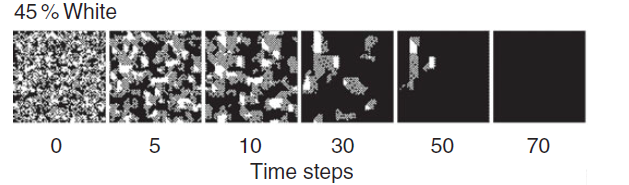
\includegraphics[width=1.0\textwidth]{mo07_fig3_maj_task.png}
	\caption[Majority Task CA]{
	An illustration of a majority task cellular automata correctly classifying the majority initial state by converging to black. Figure from \citeauthor{mo07}~\cite{mo07}.
	}
	\label{fig:maj_task}
\end{figure}

\begin{figure}[htp]
	\centering
	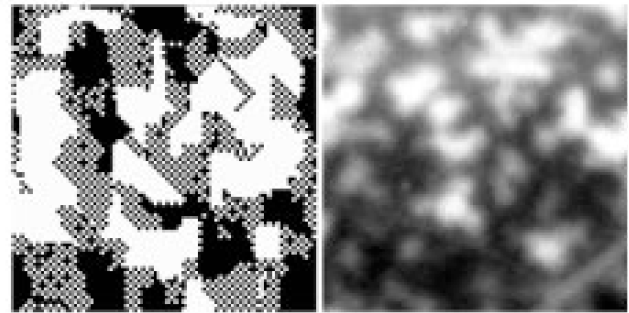
\includegraphics[width=0.75\textwidth]{me07_fig3_ca_stoma_comparison.png}
	\caption[Qualitative CA-Stomata Comparison]{
	The left image illustrates coherent state patchiness in a majority task cellular automata. The right image illustrates a similar patchiness for stomata in the plant \textit{Xanthium strumarium L}. Figure from \citeauthor{me07}~\cite{me07}.
	}
	\label{fig:ca_stoma}
\end{figure}

It is important to note however that none of these systems are guaranteed to optimally solve the majority task, and even determining whether or not a single instance will perform optimally is hard. The inherent difficulty of determining the success or failure of a given task-performing network emphasizes the importance of information granularity; in an appeal to the concept of self-organizing criticality~\cite{ba88}, small pieces of fine grain information about initial configurations may lend more insight to the global behavior of a distributed network than large but coarse bodies of information about the structure of the space. Thus, studying stomatal patchiness not only provides a step towards connecting computation to phenomenon in nature but also illustrate the central ideas of robustness and criticality.

\subsection{CA Models of Social and Ecological Dynamics}

Researchers in ecology and the social sciences often use CA models when modeling dynamics because automata models encapsulate essential features of many real-world processes. The discrete and distributed nature of CA system provide a tractable system where agents (represented by individual cells) can interact in local and overlapping neighborhoods~\cite{he98,bi07}. In particular, the local interconnections present in cellular automata models illuminate how micro-level rules can give rise to certain macro-level effects, a crucial aspect of domains such as population dynamics. Because the micro/macro relations are readily apparent in CA systems, scientists in these fields can utilize such models to not only produce quantitative simulations and predictions in but also to achieve a qualitative understanding of how the real world operates~\cite{he98}. Cellular automata are appealing because they take a ``simplistic'' approach to 
``complex'' modeling, which not only is useful in domains where details on the underlying mechanisms are not well understood (such as animal herd movement or forest fire behavior) but also reduces multi-agent systems to their fundamental one-on-one interactions~\cite{bi07,ca06}, again alluding to the importance of fine-grain information when trying to understand coarse-grain processes. 

Scientists in these fields recognize the limitations of CA models as well, as there are concerns that the discrete and uniform nature of these systems are potentially prohibitive in providing a sufficiently accurate representation of the real-world phenomena they are trying to model. In particular, there is a need for variability in both the spatial construction of the modeling environment as well as the local relationship between cells~\cite{fl01} that the regular lattice structure of traditional cellular automata do not provide. We will consider these limitations as well as work on alternative spatial configurations in more detail in Section~\ref{sec:Model}.

\subsection{Cellular Automata as Inspiration for Novel Computing Models}

Additionally, distributed CA systems have provided inspiration for new forms of computing. Computing models based on cellular automata are founded upon three fundamental principles: simplicity, ``vast parallelism'', and locality~\cite{si99}. Similar to the appeal of automata systems in dynamic modeling, CA-based computers utilize simple ``cellular'' computational units in tandem to solve complex computational tasks, can invoke parallelism on a scale that traditional parallel systems cannot achieve, and have better fault containment as well as more tolerance of imperfect input and execution due to strictly local connectivity.

An example of such a cellular-based computing is the CAM-8 architecture developed by \citeauthor{ma96}. The CAM-8 computer architecture is motivated by the idea that in order to maximize computational density, the underlying structure of the computer must mimic the basic spatial locality of physical law~\cite{ma96}. Thus, the architecture is mesh network of local CA ``compute nodes'' as they accurately represent the local interconnectivity that is present in real-world micro-physical systems. As a result, there is a correspondence between how computation is performed under the architecture and the physical implementation of the system itself. Because of this adherence to physical law, the CAM-8 architecture is particularly capable of computing spatially moving data, ideal for particle simulation and medical imaging, among others~\cite{ma96}. The goal with CAM-8 and other distributed cellular computing models is not necessarily to replace serial computers, but rather to find particular domains of problems where these alternative computing models can excel in and perhaps surpass traditional computing models.

These cellular-based computing architectures are not without their own limitations. One of the main challenges in cellular computing is being able to find local interaction rules that express the overall problem that needs to be computed. There is no good way to abstract beyond the local CA rules to provide a high-level interface for programmers to develop in, making deliberate and controlled global behavior difficult to produce. Indeed, this is the main barrier CAM-8 must overcome with in order to become a viable and practical computer architecture. There is also an issue of scalability; scaling grid size does not necessarily bring about performance scaling or even task scaling: whether or not the same level of performance on the task is maintained~\cite{si99}. Nevertheless, the potential applications in building cellular-based computational models illustrate the promise of examining robust distributed computation in natural CA-like systems.

\section{Criticality and the Emergence of Computation}
\label{sec:Crit}

\subsection{Foundations of Computation in Dynamical Systems}

What are the requisite conditions for computation to emerge from a dynamical system?
It has been shown that various CA systems can support universal computation~\cite{wf86}, but what are the particular characteristics that allow for computation to be possible? Computational constructs such as Turing machines and other equivalent entities are built upon three fundamentals that can be formulated in the dynamics of a CA system. The system must be able to support the \textit{storage} of information, with the ability to preserve information for arbitrary time periods. Information \textit{transmission} across arbitrarily long distances must also be possible in the environment. Finally, there must be some mechanism for information \textit{interaction} with the potential for information to be transformed or modified~\cite{la90}. These properties are necessary for any dynamical system, automata or otherwise, to have the capacity for computation, but are not sufficient to give rise to computation by their presence alone.
\citeauthor{la90} also establishes the notion of dynamical systems undergoing ``physical'' phase transitions between highly ordered to highly disordered dynamics, with the most interesting behavior occurring within the boundaries of this transition. This transition region is also where the three requisite properties of computation often occur. Thus, the hypothesis \citeauthor{la90} claimed is that computation can spontaneously emerge and dominate the dynamics of a physical system when such a system is at or near such a \textit{critical transition} point~\cite{la90}. 

\subsection{Metrics}
\label{subsec:metrics}
Throughout the pursuit of understanding computation in dynamical CA systems, many metrics have been utilized and created that can help quantify particular computational characteristics. We will touch on and present some of them here, with equations listed in Appendix \ref{app:Defs}.

\medskip

We will begin with a formal definition of a cellular automaton~\cite{la90}. A CA is composed of a lattice of dimension $D$ with a finite automaton present in each cell of the lattice. There is a finite neighborhood region $\mathcal{N}$, where $N = |\mathcal{N}|$ is the number of cells covered in the neighborhood region. Typical neighborhood stencils for two-dimensions are the five-cell \textit{von Neumann neighborhood} and the nine-cell \textit{Moore neighborhood} (Figure \ref{fig:neighborhoods}). Each cell contains a finite set of cell states $\Sigma$ of size $K = |\Sigma|$ and a transition function $\Delta$, which maps a set of neighborhood configurations to the cell states: $\Delta: \Sigma^N \to \Sigma$. We typically characterize a particular class of cellular automata by the number of neighbors $N$ and the number of cell states $K$. 

\begin{figure}[thp]
\centering
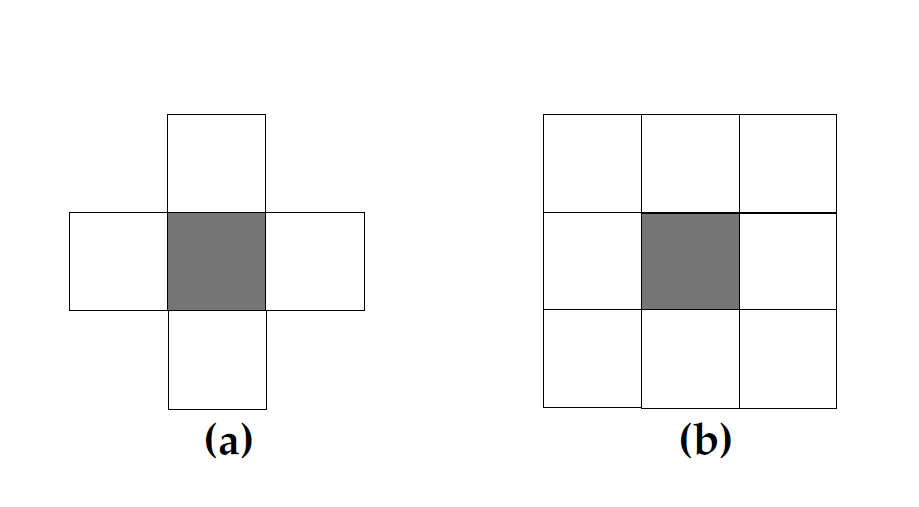
\includegraphics[width=0.75\textwidth]{mi96_fig3_neighborhoods}
\caption[CA Neighborhood Stencils]{
	(a) is the five-cell von Neumann neighborhood, (b) is the nine-cell Moore neighborhood. The gray cell is the one to be updated by a transition rule. Figure from \citeauthor{mi96}~\cite{mi96}.
}
\label{fig:neighborhoods}
\end{figure}

\medskip

\citeauthor{wf84} proposed a qualitative method for classifying CA automata behavior, with systems falling into one of four classes~\cite{mi96,wf84}:
\begin{itemize}[noitemsep, nolistsep]
\item Class I: All initial configurations relax to the same fixed, homogeneous state.
\item Class II: The CA relaxes to simple periodic structures, perhaps dependent on the initial configuration.
\item Class III: Most initial configurations degenerate to chaotic, unpredictable behavior.
\item Class IV: Some initial configurations result in complex localized structures that have the potential to be long-lived.
\end{itemize}

\citeauthor{li90b} later expands to six categories, with Class I and Class II both split into more specific subclasses. Though these are broad, rough categorizations, we expect Class IV to be the category of interest when examining potential capacity for computation in cellular automata.

\medskip
The parameter $\lambda$ (Appendix \ref{appA:lambda}) as established by \citeauthor{la90} is used to both narrow the space of CAs to consider as well as to measure the relative homogeneity or heterogeneity of a CA rule table: a completely homogeneous rule table maps all entries to a single \textit{quiescent} state whereas a completely heterogeneous rule table maps entries to random states~\cite{la90}. $\lambda$ is the fraction of the number of non-quiescent mappings in a given rule table, and can be thought of the average amount of order a given automata transition rule set possesses. Thus, $\lambda$ values range from $0$, which represents a completely homogeneous rule table to $1 - \frac{1}{K}$, which represents a completely heterogeneous table. There is also a notion of \textit{critical} $\lambda$, denoted $\lambda_c$, where the most complex dynamics tend to emerge. $\lambda_c$ and idea of criticality will be examined in more detail in Section \ref{subsec:edge_chaos}. The hypothesized relationship between $\lambda$ and Wolfram's complexity classes can be seen in Figure \ref{fig:wolfram}.

\begin{figure}[htp]
	\centering
	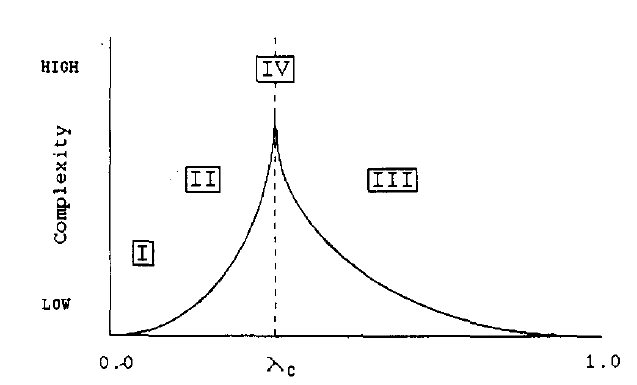
\includegraphics[width=0.75\textwidth]{la90_fig16_wolfram_classes.png}
	\caption[Wolfram's Complexity Classes]{
	The hypothesized relationship between $\lambda$ and complexity. Class IV CAs would only appear at critical levels of $\lambda$. Figure from \citeauthor{la90}~\cite{la90}.
	}
	\label{fig:wolfram}
\end{figure}

\medskip

The statistical quantity $\gamma$ (Appendix \ref{appA:gamma}) developed by \citeauthor{li90b} is another metric that describes the average asymptotic motion or spreading rate of the \textit{difference pattern} in a CA. The difference pattern is a measurement of how two different configurations on a automata lattice become either more different or more similar when applying transitions from the same rule table~\cite{li90b}. $\gamma$ can roughly be seen as the ``variance'' to $\lambda$'s ``mean'' when considering the relative order or chaos, as $\gamma$ provides finer-grain information about the dynamics of particular CA that may not be distinguishable when only considering $\lambda$.

\medskip

A common quantity used to measure the relative order in a CA system is \textit{Shannon entropy}, denoted by $H$ (Appendix \ref{appA:entrop})~\cite{la90,li90a,wo90}. We can think of Shannon entropy as measuring the amount of information present in the CA space based on the frequency of cell state occurrences; there is less information in ordered systems and more in disordered systems. Thus a completely homogeneous rule table will yield an entropy of $H = 0$ while a completely heterogeneous rule table will yield the maximum entropy possible for that particular $(N,K)$ class of automata. A natural extension to this measure is \textit{mutual information} (\ref{appA:mut_info}), defined as the correlation between two individual cell entropies~\cite{la90}. We expect some amount of mutual information being shared across cells in order for computation to be supported; too little shared information degenerates to chaotic behavior, while too much mutual information creates highly correlated structures that are too rigid to support computation.

\medskip

\textit{Mean field theory} from the description of many-body systems in physics is often used to approximate a number of the metrics described above~\cite{li90b,wo90}. The idea is to quantify a many-body system not by considering all mutual two-body interactions (which may become intractable), but rather to describe the interaction of one particle with the the rest of the system by an ``average potential'' created by the other particles. This approximation technique is particularly useful when considering classes of automata in the limit, such as in the analysis performed by \citeauthor{wo90}. Approximations for $\lambda_c$, $\gamma$, and $H$ using mean field theory can be found in Appendix \ref{appA:MFT}.

% TODO MFT citation

% TODO Peak statistics (Power Law, etc)

% TODO pattern bases definitions?

% TODO closing paragraph something along the lines of: these are some ``traditional'' methods for evaluating discrete/uniform CAs. Part of this work is finding more accurate measures when the objects of analysis are not regular, where patterns and structure cannot be utilized as a foundation for the metrics. 

\subsection{The Edge of Chaos: Investigating where Computation Emerges}
\label{subsec:edge_chaos}
\citeauthor{la90} introduces the idea that computation emerges from ``the edge of chaos,'' the critical transition region that separates ordered and chaotic behavior~\cite{la90}. His primary method of investigation is a Monte Carlo sampling of two-dimensional CAs, comparing the relationship between the parameter $\lambda$ and the average dynamical behavior of the system, measured by entropy. From both qualitative and quantitative analyses, the most interesting action in 2D CAs occurs in middling $\lambda$ values, where the \textit{transient lengths} before static structures emerge is arbitrarily long. Low levels of $\lambda$ have short transient lengths before the CA crystallizes (Figure \ref{fig:order_trans}), and high levels of $\lambda$ have short transient lengths before the CA degenerates into chaos (Figure \ref{fig:chaos_trans}). Levels of $\lambda$ in the middle however are a ``sweet spot'' of entropy (Figure \ref{fig:long_trans}); since information storage involves lowering entropy while transmission involves raising entropy, a balance must be struck in the overall system to support these foundations of computation. Mutual information is another measure that captures this same balance: if the correlation of entropy between two given cells is too high, they are overly dependent and have a tendency to crystallize, but if the correlation is too low, the cells are effectively acting independently, indicating chaos. 

\begin{figure}[htp]
\centering
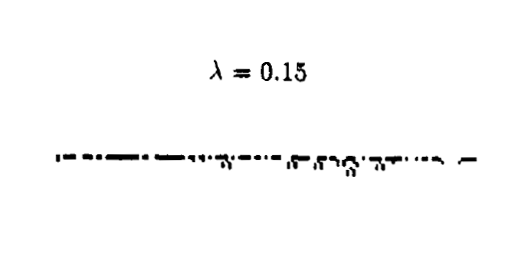
\includegraphics[width=0.5\textwidth]{ordered_transient.png}
\caption[Ordered CA Transient Length]{
The progression of a one-dimensional $N=4$, $K=5$ cellular automaton with $\lambda=0.15$ from a random initial configuration (time progresses from top to bottom). The transient length is incredibly short, with the automaton converging to a homogeneous state (all white) within four or five time steps. Figure from \citeauthor{la90} \cite{la90}.
}
\label{fig:order_trans}
\end{figure}

\begin{figure}[htp]
\centering
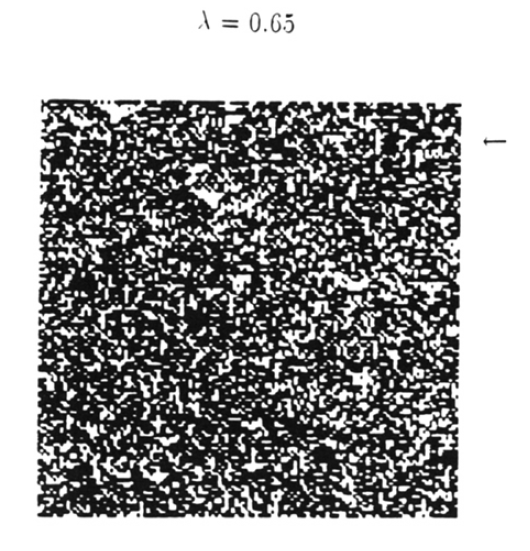
\includegraphics[width=0.5\textwidth]{chaos_transient.png}
\caption[Chaotic CA Transient Length]{
The progression of a one-dimensional $N=4$, $K=5$ cellular automaton with $\lambda=0.65$ from a random initial configuration. The transient period ends quickly (indicated by the arrow), with dynamic activity degenerating into chaos. Figure from \citeauthor{la90} \cite{la90}.
}
\label{fig:chaos_trans}
\end{figure}

\begin{figure}[htp]
\centering
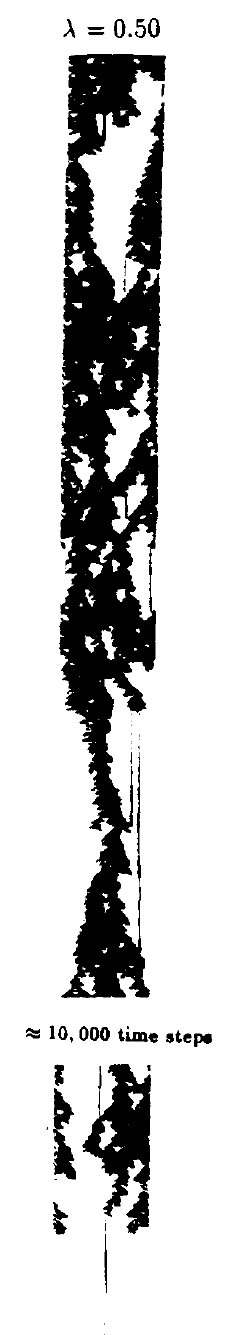
\includegraphics[width=0.20\textwidth]{long_transient.png}
\caption[Complex CA Transient Length]{
The progression of a one-dimensional $N=4$, $K=5$ cellular automaton with $\lambda=0.5$ from a random initial configuration. The transient length is quite long (over 10,000 time steps), indicative of more complex dynamical activity. Figure from \citeauthor{la90} \cite{la90}.
}
\label{fig:long_trans}
\end{figure}

Dynamical systems such as CAs exhibit characteristics that echo to the decideability of computation. CAs that live below the transition point quickly crystallize or ``freeze,'' while CAs above the point degenerate into random chaos. The behavior of dynamical systems at the fringes of the $\lambda$ spectrum can thus be determined, while CAs that live near the transition point cannot; this \textit{freezing problem} shows that it is undecideable whether or not a particular CA rule set within this complex region will either crystallize or degenerate due to the long transient lengths. Since computers are simply highly formalized dynamical systems, the classic Halting Problem can be viewed as a specific instance of the freezing problem. Through these experiments and observations on the relationship between $\lambda$ and dynamic, \citeauthor{la90} has established a bound on the complexity of dynamical systems; systems located near the edge of chaos exhibit a wide range of complex behavior that contain the foundations of computation. Thus, there is a narrow location in the $\lambda$ spectrum of dynamical systems where emergent computation can be discovered, with the maximum complexity occurring at $\lambda_c$ (Figure \ref{fig:lambda_trans}).

\begin{figure}[htp]
\centering
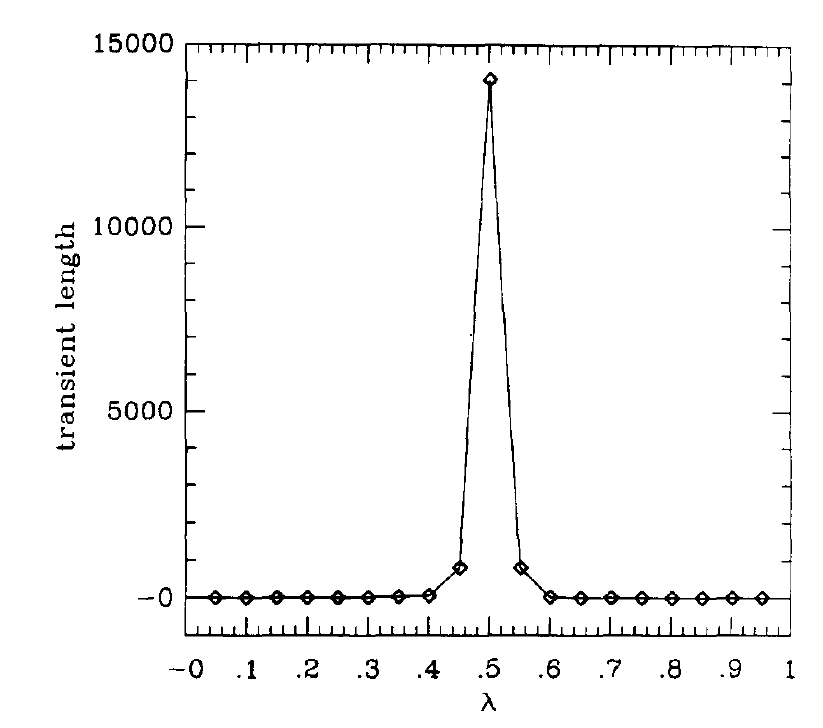
\includegraphics[width=0.5\textwidth]{la90_fig3_lambda_transient_len.png}
\caption[Lambda and Transient Length]{
Average transient length as a function of $\lambda$ for a 1D CA. The long transient lengths centered around $\lambda_c=0.5$ indicate the transition between ordered and disordered dynamics. Figure from \citeauthor{la90} \cite{la90}.
}
\label{fig:lambda_trans}
\end{figure}

Further work attempted to pinpoint precisely where the transition point occurs in a class of CA behavior, perhaps continuing along the parallels between CAs and transitions in physical systems. Utilizing mean-field theory, theoretical approximations of the entropy against $\lambda$ in two-dimensional automata made by \citeauthor{wo90} closely match previous experimental results. As the number of total possible cell states approaches $\infty$, it has been determined that there is a sharp phase transition occurring at $\lambda=0.27$, akin to first-order transitions in actual physical systems~\cite{wo90}. Perhaps this is the $\lambda_c$ point for this particular class of CAs. These results show promise in the parallels between physical systems and the dynamic behavior of cellular automata. However, to investigate this in further detail, it may be necessary to identify other statistical properties in order to fully determine the phase transition point.

Likewise, \citeauthor{li90b} examined the dynamics of CA behavior with respect to $\gamma$ in an effort to better characterize the transition region. They determined that this region between ordered and chaotic behavior is not smooth, but rather a complicated structure in of itself as values of $\gamma$ fluctuate widely within the space~\cite{li90b}. Most of the transition region is a boundary between ordered and chaotic, with abrupt jumps in behavior for CAs that cross this border. However, other areas of the region appear to have a ``thickness'' in the boundary, yielding smooth changes in statistical measures through this critical subregion (Figure \ref{fig:ca_space}). Thus \citeauthor{li90b} also come to the conclusion that $\lambda$ alone cannot specify the critical region for dynamic CA systems.

\begin{figure}[htp]
\centering
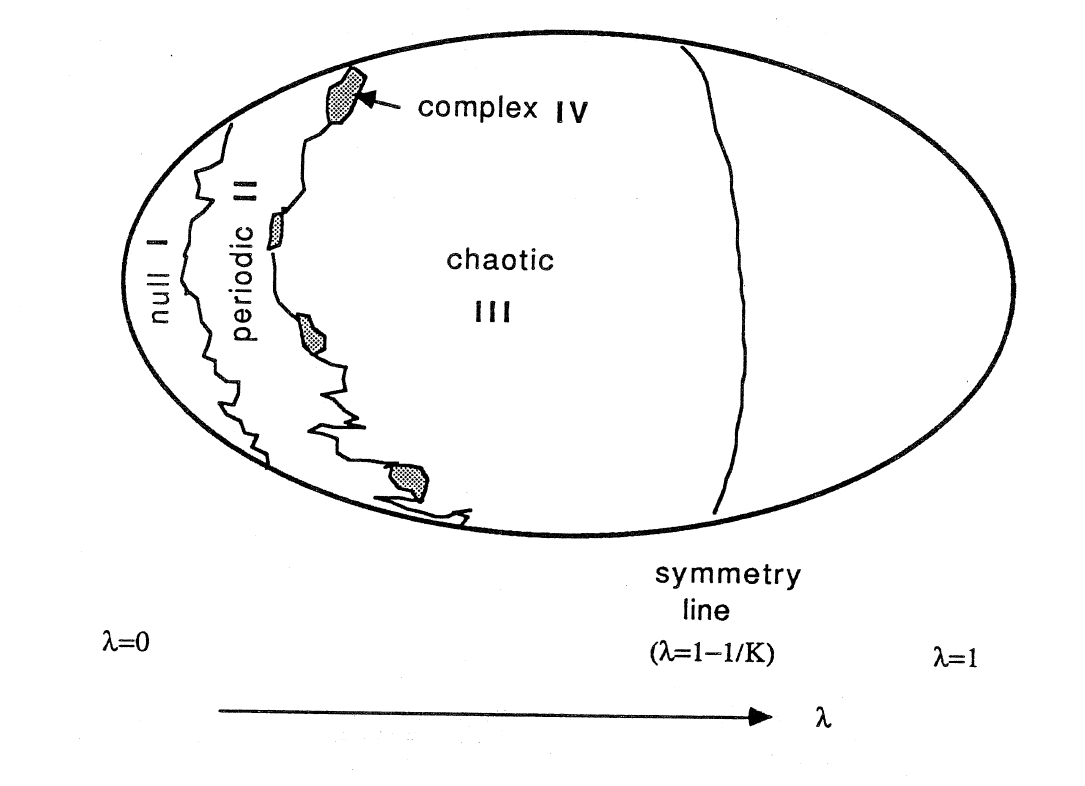
\includegraphics[width=0.75\textwidth]{li90b_fig11.png}
\caption[Hypothesized CA Space]{
A hypothesized structure of the cellular automata rule space, with the relative location of Wolfram's complexity classes listed. In most areas, the transition between class II and class III automata is sharp. However, some subregions contain a smooth transition at the boundary, where class IV automata are hypothesized to reside in. Figure adapted from \citeauthor{li90b} \cite{li90b}.
}
\label{fig:ca_space}
\end{figure}

Others have questioned whether a precise critical point where computation emerges truly exists. \citeauthor{mi93} reexamine the relationship between $\lambda$ and the dynamic behavior of ordered and unordered CAs by attempting to replicate experiments that suggest the existence of ``critical'' $\lambda_c$ in previous work by \citeauthor{pa88}. Though \citeauthor{wo90} determined that there is a convergence to a critical point in the limit of infinite state CAs, the relationship between $\lambda$ and critical regions is less clear for finite state CAs. What is important to note is that the variability of CAs at a given lambda value could be high (measured by the difference pattern spreading rate, $\gamma$), and so the behavior of a particular rule at a given value of $\lambda$ might be very different from the average behavior at that value. \citeauthor{pa88} utilizes a \textit{genetic algorithm} to evolve one-dimensional, two-state automata ($K=2, N=3$) that solve the majority task; his results indicate clustering around $\lambda_c$ in the final population of CAs, which is cited as evidence for complex behavior emerging at the boundary points. However a theoretical examination shows that, given the natural symmetry in the majority task problem, the optimal $\lambda$ value occurs at $0.5$, not at the critical $\lambda$ point. \citeauthor{mi93} then run their own genetic algorithm, showing that the best CA rules in fact cluster around $0.5$. It is important to note that for that particular class of one-dimensional, two-state automata, $\lambda = 0.5$ is considered to be in the region of chaotic CAs~\cite{mi93}. 

These results illustrate an important point: statistics that measure the behavior of these CAs may apply an implicit ``filtering bias'' on the class of automata, and so structure may be revealed under different measures that is not present under other measures, as shown by $\lambda$'s classification of the optimal CAs for the majority task as chaotic. \citeauthor{la90}'s hypothesis that $\lambda$ correlates with computational ability appears to need refinement: $\lambda$ may very well correlated with the average behavior of CAs but what is the significance of  ``average behavior,''  especially when $\gamma$ is high in the critical regions of interest? For a given $N$ and $K$, CAs that have the potential to compute may reside in a wide range of $\lambda$ values, illustrating the need for a more precise metric. \citeauthor{mi93} also stress that the focus should be harnessing the computation ``naturally'' present within a CA rather than attempting to impose traditional definitions of computation upon them. 

Nevertheless, the relationship between critical regions and computation in general remains important and needs to be closely examined at a finer grain. Instead of considering the average behavior of automata, \citeauthor{cr93} decompose and filter the spatial configurations of one-dimensional CAs as they move through time. The central goal of their work is to distill a seemingly turbulent system by finding a \textit{pattern basis} representation of the CA space that will serve as the backdrop for potential coherent structures present in the system to be identified~\cite{cr93}. These pattern bases form \textit{regular domains} that are \textit{temporally invariant}, where the CA rule table maps configurations within a regular domain to the same regular domain~\cite{mi96}. With these stable domains identified, they can be filtered out of the space-time diagrams, with the dynamics of interest becoming apparent at the boundaries between regular domains, which are particle-like in behavior~\cite{cr93}. Thus, the dynamics of a CA can be examined in this manner to illuminate underlying structure, providing more useful and finer-grained information than simply classifying the system as ordered or chaotic as shown in Figure \ref{fig:ca_filter}. \citeauthor{cr93} calls these domains and structures the \textit{intrinsic computation} of the CA, as they can be understood in computational terms regardless of the global computation taking place in the CA~\cite{mi96}. The intrinsic computation in itself is an interesting unit of analysis, capable of generating rich interactions at the domain borders that may in fact cause coordinated behavior to emerge~\cite{cr95}. Again, this stresses the importance of information granularity, as the presence of many smaller regular domains that have inherently different structures in the CA space can cause statistics collected across the global domain to be misleading~\cite{cr93}.

\begin{figure}[htp]
\centering
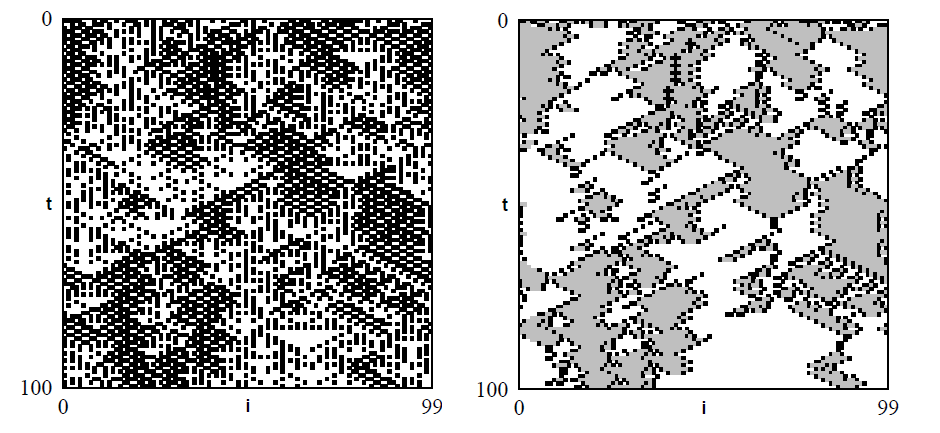
\includegraphics[width=0.9\textwidth]{cr93_fig3.png}
\caption[Filtered CA Behavior]{
Space-time plots for a $K=5$, $N=2$ 1D cellular automata with a random initial configuration of lattice size 100. The left image illustrates the unfiltered progression of the CA, while the right image illustrates the same behavior, filtered by two regular domains indicated by white and gray. Figure adapted from \citeauthor{cr93}~\cite{cr93}.
}
\label{fig:ca_filter}
\end{figure}

Throughout our exploration of computation in distributed dynamic systems, we often see a delicate balance struck between order and chaos in order to support complex behavior: information must be both propagated (high entropy) and stored (low entropy), and minute alterations in local configurations can have catalytic global effects. What happens when this balance is disturbed? Thus far we have only considered highly regular environments for computation in CA systems, with uniform lattice grids and rule tables. Do these systems behave robustly when the environments are not well-structured? Dynamic natural systems serve as ``the ultimate proof of concept,'' as they are able to function despite residing in environments (the real world) that are inherently noisy and irregular~\cite{si99}. We'll look first to inspiration from nature when considering fault tolerance in computing CA systems. 

% TODO more on sandpile analogy

% TODO elaborate on regular domains in the metrics section?

\section{Robustness in Face of Irregularity}
\label{sec:Robust}

\subsection{Stomatal Dynamics Revisited: Utilizing Environmental Noise}
We begin our review of robustness by revisiting plant stomatal dynamics. Unlike technological systems, biological systems such as stomatal arrays on plant leaves are often able to manage variable environments ``innately,'' without external intervention or control. Indeed, though stomatal systems behave similarly to majority task CAs as noted earlier in Section \ref{subsec:Stoma}, they face a number of irregularities not accounted for in the CA models such as \textit{heterogeneous interactions}, where local interactions may not be uniform due to stomatal size, orientation, and spacing,  or \textit{modularity}, where leaf veins cause stomata to be subdivided into modules that interact at a level beyond individual stoma interaction~\cite{me07}. Additionally, the stomatal systems must handle temporal \textit{state noise}, where there is unavoidable variability and imprecision in the stomatal functioning itself across time. Thus, \citeauthor{me07} examine the behavior and performance of stomatal-inspired majority task CAs in environments designed to mimic the irregularities plant stomata have to contend with.

When considering the majority task, most initial configurations are relatively easy for CAs to classify correctly, where there are a large proportion of either ON or OFF cells present in the space. Unsurprisingly, the most difficult cases are when the density of on and off cells are roughly equivalent. \citeauthor{me07} note that these hard cases often cause patchiness and are solved correctly only when the patches travel coherently across the CA space, emphasizing the importance of information transfer when supporting task performance in these locally connected networks. Unsuccessful CAs often have ``stuck'' patches that are unable to be resolved. Irregularities in the form of heterogeneous interactions, simulated by nonuniform rule tables and random connectivity, and modularity, simulated by grafting together \textit{mosaic networks} of modules, both reduce the performance of the task CAs but do not cripple them~\cite{me07}. Perhaps most surprisingly, the majority task CAs actually \textit{improve} in performance when small amounts of state noise are introduced to the system while other defects are present. \citeauthor{me07} hypothesize that this is because the state noise cause small perturbations in the system, stimulating movement and perhaps freeing previously stuck patches to move about the space once more. We have seen how small changes can snowball and sweep through entire the entire CA space, and it appears that natural systems embrace noise and use it to their advantage. Indeed, randomness appears essential in facilitating the self-sustaining and self-informing function of decentralized biological systems~\cite{mi05}. We will turn to \citeauthor{mi05}'s analysis of how these systems might operate to illustrate how such structures can maintain themselves in such complex environments despite the lack of central control.

%TODO Table 1 of me07 for noise improvement

\subsection{Redundancy in Decentralized Systems}
\citeauthor{mi05} presents two instances of decentralized systems, the human immune system and ant colonies, which perform complex tasks via ``adaptive self-awareness:'' global information about the system dynamically shapes and feeds back to the movements and actions of the lower level components. What is interesting about these systems is that single agents act naively, tending to conform to what the dominant behavior is locally: for example, an ant in an ant colony will have an increased probability of switching to and working on a task if it observes many other ants in its immediate environment working on it~\cite{mi05}. However, it is the probabilistic aspect of these decisions, the idea of sampling a small ``neighborhood,'' that allow the complex behavior to emerge. Similar to an ant's local sampling, a lymphocyte will bond with molecules indicative of pathogens it encounters locally and will reproduce proportional to the strength of the bond it forms, facilitating a Darwinian process in that the best lymphocytes for combating the pathogen will emerge on a system-wide scale.

From studying immune systems and ant colonies, \citeauthor{mi05} emphasizes the need for randomness and probabilistic decisions in order for controlled behavior to occur: these systems are not just robust to variations in their environment, but actually require irregularities and noise to function properly. Additionally, they illustrate the importance of redundancy and sampling. A single lymphocyte or ant is a fragile unit, and so the global system cannot be dependent on any specific agent present within its system. Instead, there is an inherent redundancy within the system, with many agents sampling their local environments, yielding independent, fine-grained behavior that only become significant when considered globally~\cite{mi05}. Thus, the individual components do not rely on each other making the system robust to faults, yet the overall behavior is highly coordinated. 

We see the ideas of redundancy and random noise come into play again in \citeauthor{ac14}'s efforts to mimic natural robustness to variability in their \textit{Moveable Feast Machine,} a dynamic CA-based architecture designed with the hope of producing ``indefinitely scalable,'' robust computing. The computational entities, called \textit{atoms}, move about probabilistically in a two dimensional grid, independently and asynchronously acting on their local neighborhood. A sorting routine implemented within this architecture, \textit{demon horde sort}, utilizes ``hoarder'' atoms that sort values spatially: the hoarders move about randomly in space, pushing locally higher values above itself, and locally lower values below itself~\cite{ac12}. Like the lymphocytes and ants, the hoarders act individually, only producing the desired end result of a sorted list when considered on a global scale. Since the behavior of each hoarder is essentially the same, a space filled with many hoarder atoms will contain a large amount of functional redundancy that allow the system to tolerate many environmental perturbations, such as the destruction of hoarder atoms~\cite{ac14}. This can be thought of as a robust parallelized bubble sort in a sense, reaping the performance benefits of non-sequential computation while also being robust to faults~\cite{ac13,ch89}. \citeauthor{ac14}'s system is facilitated by the same concepts \citeauthor{mi05} identified in her work: decentralized systems harness the power of noise and redundancy to self-organize and perform complex tasks.

However, we feel that there is another potential source of variability that has not been considered as extensively in the work presented above: spatial irregularity. Both \citeauthor{me07} and \citeauthor{ac14} draw inspiration from biological systems yet continue to utilize uniform grids as their spatial representations. Natural dynamical systems do not typically operate in a uniform lattice, so this may be a limiting assumption. Thus, we will present previous work considering spatial representations and how they may potentially impact the dynamics of the distributed CA systems we have been examining.

%TODO Chandy reference, UNITY programming language, ch89
%TODO si04, Studying Fault Tolerance

\section{Spatial Representations and Modeling of CAs}
\label{sec:Model}
\subsection{Limitations of Traditional CA Spatial Representations}

Returning to the applied CA models from section \ref{sec:Motiv}, there are some who question the viability of traditional CA models as adequate simulations of real-world phenomenon. Beyond the obvious limitation that real-world systems rarely exist in regular grids, a primary concern is that the grid predefines a fixed spatial scale, making representations of both cells and the environment itself inflexible~\cite{he98}. In the case of modeling population dynamics, if the cell size is on the scale of the agent we are modeling, building and simulating on a grid that is adequately sized for modeling the movement of the agent often becomes intractable~\cite{bi07}. On the other hand, if the cell size is larger than the agents being modeled, the structure of the grid has placed an arbitrary bound on the population density it can represent.

Additionally, the neighborhood definitions are entirely dependent on the structure of the grid configuration, making it difficult to define alternative neighborhood stencils beyond variations of the standard Moore or Von Neumann neighborhoods. The local connectivity can be varied by using different shapes such as hexagons as tiles, but the number of neighbors per cells are still restricted to the same amount across the space. Thus, in order to support richer neighborhood interactions, the size of the neighborhood must be variable while still respecting the local connectivity of the grid. We consider a first step in this direction by examining alternative formulations of the Game of Life.

% TODO more here

\subsection{Spatial Variation of Conway's Game of Life}
\label{subsec:gol}
The Game of Life, discovered by John Conway, is a $K=2$, $N=9$ two-dimensional cellular automaton that is particularly remarkable because of both the rich emergent structures it can generate as well as its Turing universality~\cite{ga70}. Most instances of the Game of Life are played on regular, two dimensional lattices; what changes in behavior occur when it is simulated on an aperiodic \textit{Penrose tiling}? \citeauthor{hi05} examined this variation, and in particular ran experiments that explored the \textit{lifetimes} (number of generations until stabilization) as well as  \textit{ash densities} (the fraction of ``on'' cells in a stabilized configuration) of random initial configurations. The Game of Life on the Penrose tiles have lifetimes that are much shorter and ash accumulation half as dense as games played on the regular lattice~\cite{hi05}; this is likely due to the irregularity in the tiling distribution, illustrating that at least in this instance, the variable neighborhood sizes across the grid make it more difficult to maintain coherent structures. It should be noted however that \citeauthor{hi05} directly translated the rules of the Game of Life onto the Penrose tiling without any modification, which may not be appropriate since a given cell may have either eight or nine neighbors as opposed to the constant eight neighbors in traditional Life instances. An alternative rule set would be to define the ``living'' criteria based on a ratio or percentage of live cells in the surrounding area, as it would produce appropriately dynamic behavior that aligns with the variability in the tilings. This addition is an extension on these initial experiments that may be more revealing to the overall relationship between the Game of Life played on a grid and more irregular environments like Penrose tiles. 

To take spatial representations to one extreme, the concept of a grid can be removed altogether. \textit{SmoothLife} is the result, where instead of cells on a grid individual points within the Cartesian space is considered and transition rules are defined for a point's circular neighborhood~\cite{ra11}. In SmoothLife's spatial representation, Euclidean distance is respected in regard to neighborhood definitions resulting in a true spatial representation of connectivity. Unfortunately, SmoothLife represents too radical a shift away from the discrete dynamic systems we have been considering with the lack of spatial structure entirely. Ideally, spatial representations of Euclidean distance and resulting neighborhood connections should be preserved while still maintaining a discrete structure. Voronoi diagrams possess these exactly traits, and so we will consider Voronoi-based CA systems next.

%TODO elaboration

\subsection{Voronoi Representations of CA}
\label{subsec:ModelVoronoiRep}
First, we review the basic idea of Voronoi diagrams. In order to construct a diagram, a set of \textit{generator points} are placed in the plane. The cell defined by a generator point $i$ is defined as the area containing all points of the plane that are closer to $i$ than any other point with regards to Euclidean distance (Figure \ref{fig:voronoi})~\cite{ok09}. In the realm of Geographic Information Systems, Voronoi CA systems have been utilized to explore irregular spatial patterns that occur in the real world~\cite{ca06,sh00}. \citeauthor{sh00} suggest that the main barrier that prevents CAs from being applied in the real world is that CAs cannot provide a way to handle irregular, spatially defined neighborhood relations; Voronoi-based CAs appear to be a solution to this fundamental problem. Furthermore, due to their nice spatial properties, Voronoi diagrams are often utilized in models of various natural structures, such as cells~\cite{ok09}. Though there has been extensive work examining computation in regular dynamical systems (Section \ref{sec:Crit}) and numerous applications of CAs both applied to and derived from nature (Section \ref{sec:Motiv}), there has been little work done analyzing how biologically plausible spatial representations such as Voronoi diagrams can impact computation and dynamics within a CA system. \citeauthor{fl01} provide one such analysis in the context of modeling social dynamics.

\begin{figure}[htp]
\centering
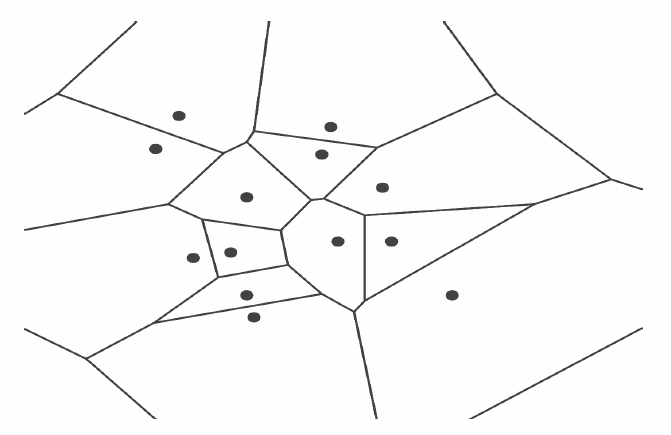
\includegraphics[width=0.5\textwidth]{wh03_fig1_voronoi}
\caption[Voronoi Diagram]{
	A voronoi diagram with its corresponding generator points. Figure adapted from \citeauthor{wh03}~\cite{wh03}.
}
\label{fig:voronoi}
\end{figure}

\citeauthor{fl01} simulate several social dynamics interactions through CA systems ran on both regular grids and Voronoi diagram analogs. The same global behavior was preserved in the Voronoi cases, though the dynamics took a longer time to converge to stabilized behavior relative to the regular grid case~\cite{fl01}. Though only a specific class of computational tasks were tested, the conclusion that these social dynamics tasks are robust to variation in grid structure leads us to the beginning stages of establishing some form of equivalence between classes of irregular and regular grid structures. Additionally, examining the spatial behavior of cells in the Voronoi case revealed some interesting patterns. Because of variations in the local structuring within the Voronoi diagrams, some areas of the irregular grid never participate in computation even when completely surrounded by computing cells, resisting all outside influences (Figure~\ref{fig:dead_cells})~\cite{fl01}. This ``dead cell'' phenomenon provides evidence that the spatial properties inherent in Voronoi diagrams can impact the system's dynamics beyond variations in cell neighborhood connectivity.
Additionally, the potential presence of dead cells along with the randomness produced by generating grids through generator points make Voronoi diagrams an interesting way of introducing variability to a cellular automata as it implicitly encodes some irregular features we have explored in Section \ref{sec:Robust}. However, further work is needed to thoroughly investigate the impact of different spatial representations on the complex behavior and computation in dynamic, decentralized systems. 
%Thus, one of the main goals of this work is apply the rigorous analysis previously seen (Section \ref{sec:Crit}) concerning emergent computation on spatially diverse systems such as Voronoi-based automata in pursuit of illuminating how natural systems can compute within such noisy environments.

\begin{figure}[htp]
\centering
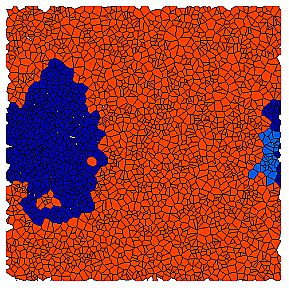
\includegraphics[width=0.75\textwidth]{fl01_fig9_color.jpg}
\caption[``Dead Cells'' in Voronoi CA]{
An irregular cellular automaton modeling cooperation dynamics in its stable state. Cooperating cells are blue and non-cooperating cells are red. Though the expected end state in this simulation on a regular grid would be a homogeneous cluster of cooperation, there are cells completely surrounded by cooperating neighbors that resist participating in the computation. Figure from \citeauthor{fl01}~\cite{fl01}.
}
\label{fig:dead_cells}
\end{figure}

\section{Summary}
\label{sec:PrevSum} 

We have seen throughout this review that work on the computational dynamics of distributed natural systems is a two-way street, 
%TODO right phrasing?
with researchers both utilizing cellular automata to investigate complex behavior in natural systems as well as drawing inspiration from nature to build more robust and efficient ``cellular computers.'' Additionally, there has been extensive work concerning how dynamic systems can give rise to computation with an abundance of metrics that can be used to analyze such systems. It would be reasonable to apply the measures from these computational criticality studies to attempt to understand natural systems. Unfortunately, there is not a clear ``mapping'' between the foundational structures of cellular automata and dynamical natural systems. Assumptions cannot be made about a potential correspondence between local connections, transition rules, or spatial orientation when CAs and natural systems operate within such contrary environments: the control and precision of computer simulation versus the noise and inconsistency of the real world. For example, the spatial structure of cellular automata is limiting when utilizing them as a model (Section \ref{sec:Model}), which is why researchers in specific modeling domains have explored removing the lattice regularity of CAs in order to observe the impact that structural assumption has on the dynamic behavior of the system.

%TODO "fuzziness"?
There is inherent imprecision when dealing with natural systems, which makes utilizing the criticality statistics problematic. The definitions of metrics like $\lambda$ and $\gamma$ as well as the notion of average dynamic behavior can be difficult translate to systems where there are no structural uniformities that can serve as a foundation for measurement. We have to adapt these metrics to the domain of irregular cellular automata in order to properly investigate the nature of computation in such systems. Perhaps there is some sort of functional equivalence between regular and irregular CAs, or perhaps they are separate classes of dynamical systems. Thus, this work will take some first steps towards resolving the complexion of this relationship. Our goal is to examine and identify potentially fundamental differences or equivalences between irregular and traditional cellular automata in the pursuit of understanding how natural decentralized systems can compute ``in the wild.''

%TODO: is hashlife ``exploiting regularities'' example appropriate in the summary?

%TODO: are ``supplemental'' figures necessary (ie neighborhood stencils, general voronoi diagram?)

% How much of Voronoi work goes in the previous work section, how much goes in later parts of the thesis?

% TODO Ga70
\processdelayedfloats

\chapter{System Design}
\label{ch:System}

In this chapter, we will give an overview of the collection of tools we have built and utilized for our exploration of irregular CA systems. The goal is to provide enough information so that any experiments described in later chapters can be replicated. 
%TODO insert specific chapters here

\section{System Overview}
\label{sec:SysOverview}

Our CA simulation platform follows an event-driven architecture written in C++; actions are placed on a queue and are performed one at a time. The event queue structure allows us to easily interleave actions in between time steps of a CA simulation; for example, we can take snapshots of the grid state or dump measurements to file in between time steps at any frequency we wish.

%TODO move around?
We designed this system primarily with flexibility in mind. Modular components and data structures can easily be swapped in and out of the simulation platform, giving us fine-grained control over the experiments we are running. Performance is not a major concern, so long as simulations and experiments can complete within a reasonable amount of time: for reference an experiment that runs 1,000 simulations 500 time steps each, writing data to disk at every time step for all simulations takes a few hours in total to complete.

%A CA simulation begins by reading in an input grid file, initializing all 

Termination of the CA simulation occurs either when a maximum time step is reached, or when a grid state is repeated. We track grid states by walking through all cells on a grid in a consistent order, appending each cell state to a string array and then passing the resulting string through a hash function. We keep a history of these hashes along with the time step they occur, and terminate the simulation if a hash is ever repeated. Recording the time step also allows us to track the periodicity of any potential oscillating structures occurring within the simulation.

We execute rule table updates across the grid in a ``spreading activation'' fashion in order to increase the performance of the simulator. Instead of visiting and updating each cell, we track which cells changed state in the previous time step and place those cells along with their neighbors in a ``change'' list. When updating the graph for the next time step, we only apply the transition rule to cells in the list. We then repeat this process, updating the list with any cells and their neighbors that have changed state. We initialize the change list at the beginning of the simulation to all cells in the grid. This method of applying updates allows us to only consider cells that could potentially change, saving time throughout the CA simulation especially if the grid is large. 

\subsection{Structures}
Our CA simulation platform consists of a collection of data structures that are utilized in tandem to run the simulation. The most essential structures are briefly described below.

\begin{itemize}

\item \textbf{Grid Generators:} The \texttt{GridGenerator} structure stores both the geometric representation of a grid and the graph representation of a grid. The graph is implemented as an adjacency list as we expect the graph of a CA grid to be relatively sparse due to the strictly local connectivity.

\item \textbf{Stencil:} A \texttt{Stencil} determines the local neighborhood for each cell in a Grid. Possible stencils include ``generalized'' von Neumman and Moore neighborhoods or ``continuous'' stencils that weight neighbors by their distance from the center cell.

\item \textbf{Rule Table:} A \texttt{RuleTable} represents a transition rule, utilizing a Stencil to determine a cell's neighborhood and compute its next state.

\item \textbf{Geometry Maps:} Maps and reverse maps from labels to geometric objects such as \texttt{Points}, \texttt{Edges}, and \texttt{Faces} are maintained for easy object access and grid manipulation.

\end{itemize}

Grid Generators will be reviewed in more detail in Section \ref{sec:GridGen}, while Stencils and Rule Tables will be discussed in Section \ref{sec:StencilGen}. A schematic of our overall program architecture is pictured in Figure \ref{fig:sys_arch}.

\begin{figure}[htp]
\centering
%Build System Schematic picture
%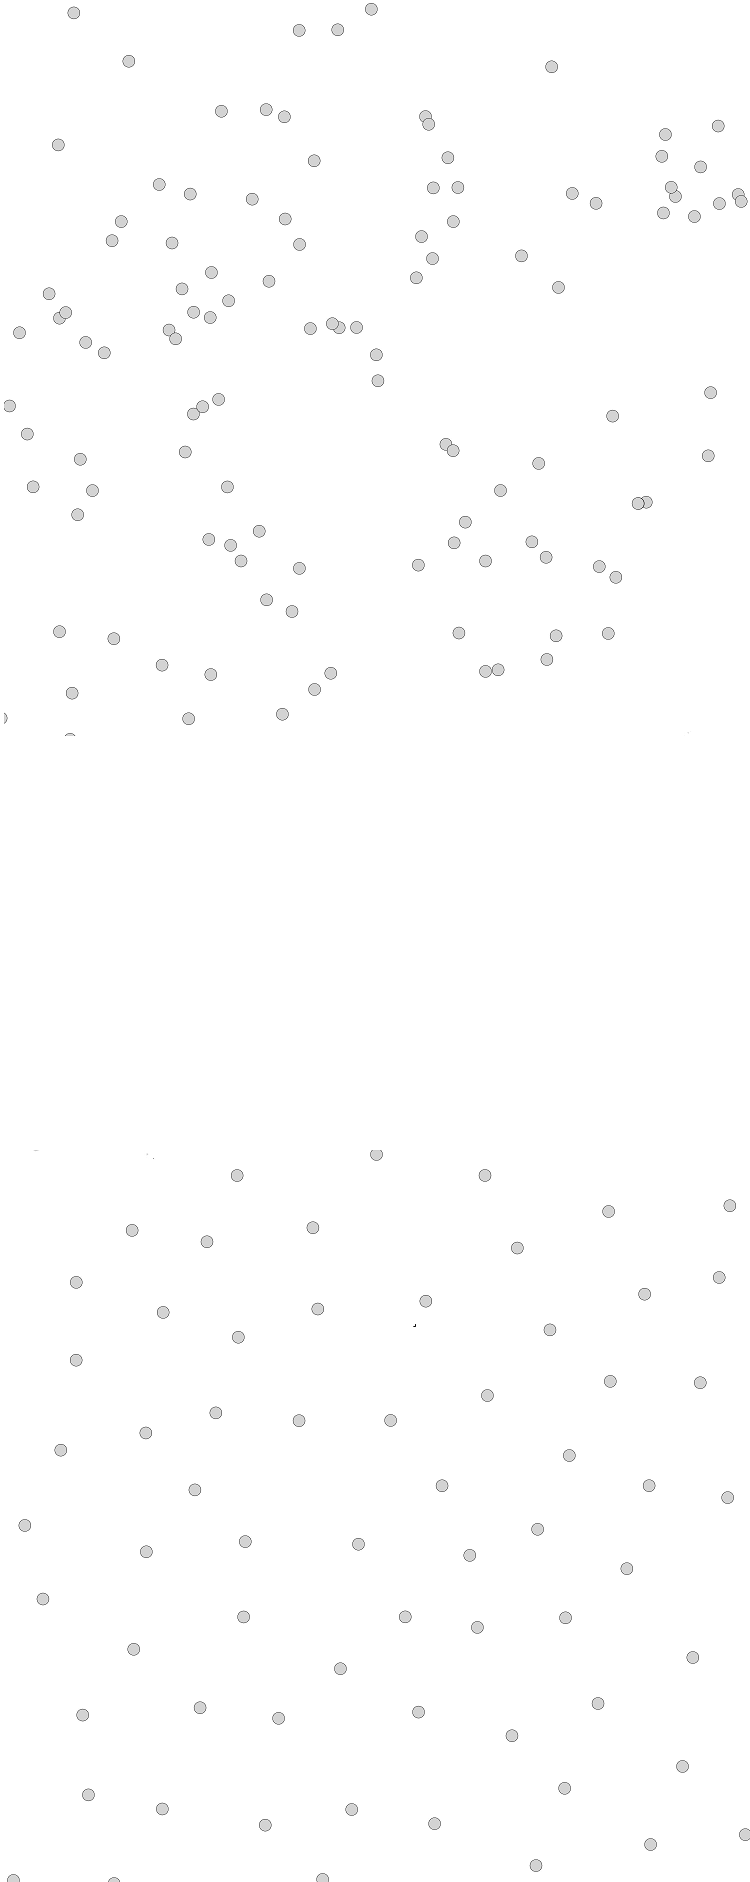
\includegraphics[width=0.4\textwidth]{gen_pts_v2}
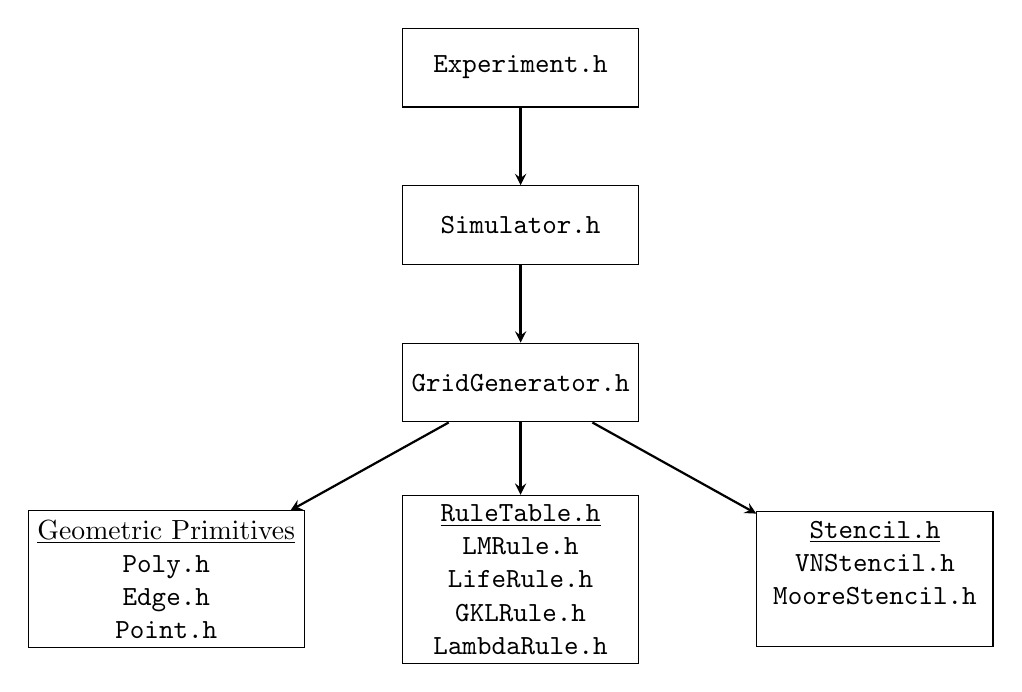
\begin{tikzpicture}[node distance=2cm]
\node (expr) [process] {\texttt{Experiment.h}};

\node (sim) [process, below of=expr] {\texttt{Simulator.h}};

\node (grid_gen) [process, below of=sim] {\texttt{GridGenerator.h}};

\node (rule_table) [process, align=center, below of=grid_gen, yshift=-0.5cm] {
	\underline{\texttt{RuleTable.h}}\\
	\texttt{LMRule.h}\\
	\texttt{LifeRule.h}\\
	\texttt{GKLRule.h}\\
	\texttt{LambdaRule.h}
};

\node (stencil) [process, align=center, right of=rule_table, xshift=2.5cm] {
	\underline{\texttt{Stencil.h}}\\
	\texttt{VNStencil.h}\\
	\texttt{MooreStencil.h}\\
};

\node (geo) [process, left of=rule_table, align=center, xshift=-2.5cm] {
	\underline{Geometric Primitives}\\
	\texttt{Poly.h}\\
	\texttt{Edge.h}\\
	\texttt{Point.h}
};

\draw [arrow] (expr) -- (sim);
\draw [arrow] (sim) -- (grid_gen);
\draw [arrow] (grid_gen) -- (rule_table);
\draw [arrow] (grid_gen) -- (stencil);
\draw [arrow] (grid_gen) -- (geo);

\end{tikzpicture}

\caption[CA Simulation Platform Architecture]{
	A schematic of our CA simulation platform. Arrows represent dependencies of classes, and boxes contain both the base class and some of its derived classes commonly used in the system.
}
\label{fig:sys_arch}
\end{figure}

\subsection{Input/Output Files and Running Our System}

We have a standardized format for storing and reading in grid configurations, which allows us to easily pause and restore CA simulations as well as save and transfer them across different machines. A representative input grid file can be found in Appendix \ref{appB:grid_in}. The visual representation of our grids are built by creating graph descriptions for \textbf{neato}, a graph layout program part of the Graphviz drawing package~\cite{el01}. Images of our neato grid representations can be found in Section \ref{sec:GridGen}. Measured statistics are exported to .csv files and analyzed using Python with packages from the SciPy ecosystem~\cite{jo14}.

We utilize the GNU C library package \texttt{getopt} to pass Unix-style command line arguments to our system, allowing experiments to be easily scripted and batched across multiple machines.

\section{Grid Generation}
\label{sec:GridGen}

In this section we'll describe the algorithms utilized to generate the various grids we run CA simulations on.

\subsection{Penrose Tilings}
To generate Penrose Tilings and Penrose-connected graphs, we use inflation processes to recursively generate the tiling. \citeauthor{ro71}'s triangle recursive decomposition technique is utilized to draw both kite/dart and thin/thick rhomb tilings, except full tiles are drawn instead of individual triangles~\cite{ro71}. Though drawing full tiles will likely result in tiles being considered and drawn multiple times, we avoid this by marking faces as they are drawn, only keeping a single copy of each face. As in all our grid generation programs, we track geometric primitives (\texttt{Point}, \texttt{Edge}, \texttt{Face}) to make generating our standard grid input file straightforward.

TODO more detail?

\subsection{Delaunay Triangulations and Voronoi Diagrams}
The goal with building grids using Voronoi diagrams is to produce irregular grids that still respect Euclidean distance, as discussed in Section \ref{subsec:ModelVoronoiRep}. Given a set of \textit{generator points} $\{p_1, ..., p_n\}$ in the plane, a Voronoi polygon $V_k$ corresponding to a generator point $p_k$ consists of all points whose distance to $p_k$ is less than its distance to any other generator point. Thus, we can partition the plane into Voronoi polygons that correspond to every generator point, producing a \textit{Voronoi Diagram}. These polygons will serve as the cells in our CA simulations. 

The first step in the process to generate a Voronoi-based grid is to produce generator points. Though a simple uniform random distribution of points in the plane will generate a valid Voronoi Diagram, the resulting grid may have undesirable geometric properties due to the potential for points to clump together. Instead, we can utilize a method called \textit{Poisson Disk Sampling} to generate random points that are guaranteed to be at least some specified distance apart from each other~\cite{br07}. Points created by this method will necessarily avoid clumping, illustrated in Figure \ref{fig:pt_gen}.

\begin{figure}[htp]
\centering

\includegraphics[width=0.4\textwidth]{ch3_figs/gen_pts_v2}
\caption[Random Point Generation]{
	On top, a random uniform distribution of points. On bottom, a random distribution of points generated by Poisson Disk Sampling.
}
\label{fig:pt_gen}
\end{figure}

Once we have a set of generator points, we construct the dual graph of the Voronoi Diagram, known as the \textit{Delaunay Triangulation}. The Delaunay Triangulation of a set of points $\{p_1, ..., p_n\}$ in the plane is a triangulation such that no point $p_k$ resides inside the circumcircle of a triangle; an edge $e$ is considered to be \textit{locally Delaunay} if the two triangles that share $e$ as a common edge satisfy the circumcircle condition~\cite{de11}. We construct this dual graph first because (1) the edges of the Delaunay Triangulation exactly correspond to the graph connectivity of the Voronoi grid produced by the set of points and (2) the Voronoi Diagram is easy to construct from the triangulation. We utilize the \textit{flip algorithm} to construct the Delaunay Triangulation: beginning with an arbitrary triangulation, edges that are not locally Delaunay are ``flipped'' such that they are locally Delaunay. Once there are no more edges to be flipped, then the resulting triangulation must be a Delaunay Triangulation~\cite{ed08}. Though the flip algorithm is not the fastest Delaunay Triangulation algorithm, it is straightforward, requires no auxiliary data structures, and performs well enough for our purposes.

Given a Delaunay Triangulation, we can produce its corresponding Voronoi Diagram by calculating the circumcenter of each Delaunay triangle and creating an edge between the circumcenters of adjacent triangles~\cite{de11,ed08}. The circumcenters of the triangles correspond to Voronoi polygon vertices, so we obtain valid Voronoi regions. Thus we have obtained both the graph representation and the geometric representation of a Voronoi-based grid. An illustration of this process is shown in Figure \ref{fig:voronoi_gen}.

\begin{figure}[htp]
\centering
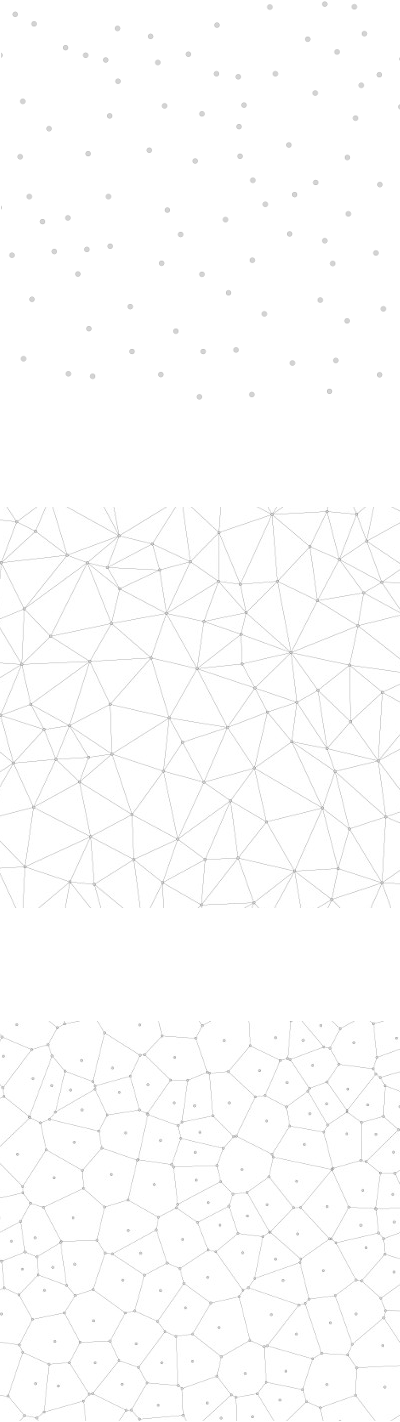
\includegraphics[width=0.4\textwidth]{ch3_figs/voronoi_generation}
\caption[Voronoi Diagram Generation]{
	The Voronoi Diagram construction process. We begin with a random set of points (top), compute the Delaunay Triangulation (center), and subsequently the Voronoi Diagram (bottom).

}
\label{fig:voronoi_gen}
\end{figure}
\subsection{Voronoi Quadrilaterals}
\label{subsec:vquad}
Experiments and simulations involving $\lambda$ require static neighborhood sizes across all cells in the grid. One way we address this requirement is by generating irregular grids that have cells of the same number of sides. Specifically, given a Voronoi Diagram we can further partition the region such that all cells in the plane are quadrilaterals. This conversion is accomplished by taking two edge-adjacent Voronoi polygons and forming a quad from the two generator points and the end points of the shared common edge between the polygons (Figure \ref{fig:vquad_gen})~\cite{am10}. As long as the given Voronoi Diagram is ``well-formed,'' specifically with all generator points placed at least some minimum radius from each other, this quadrilateral generation is possible across an entire Voronoi diagram, as seen in Figure \ref{fig:vquad_grid}. Note that though cells in the resulting \textit{VQuad} grid always share edges with four other neighboring cells (excluding the boundary) resulting in uniform generalized von Neumman neighborhood sizes across the grid, the number of cells they share vertices with are variable. This variability in vertex adjacency is partially due to the presence of concave quadrilaterals in the resulting grid. %TODO tessellation right here?

\begin{figure}[htp]
\centering
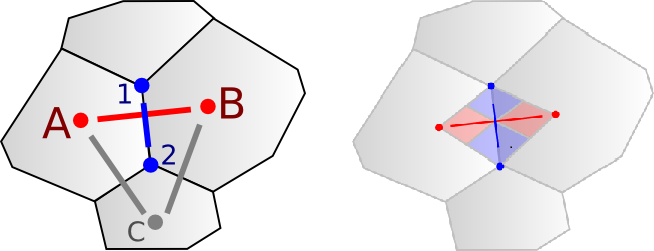
\includegraphics[width=0.75\textwidth]{ch3_figs/vquad_generation}
\caption[Voronoi Quad Generation]{
	An illustration of the Voronoi quadrilateral creation process. Generator points $A$ and $B$ are connected with the shared edge endpoints $1$ and $2$ to create the quadrilateral pictured on the right. Figure adapted from \citeauthor{am10}~\cite{am10}. 
}
\label{fig:vquad_gen}
\end{figure}

\begin{figure}[htp]
\centering
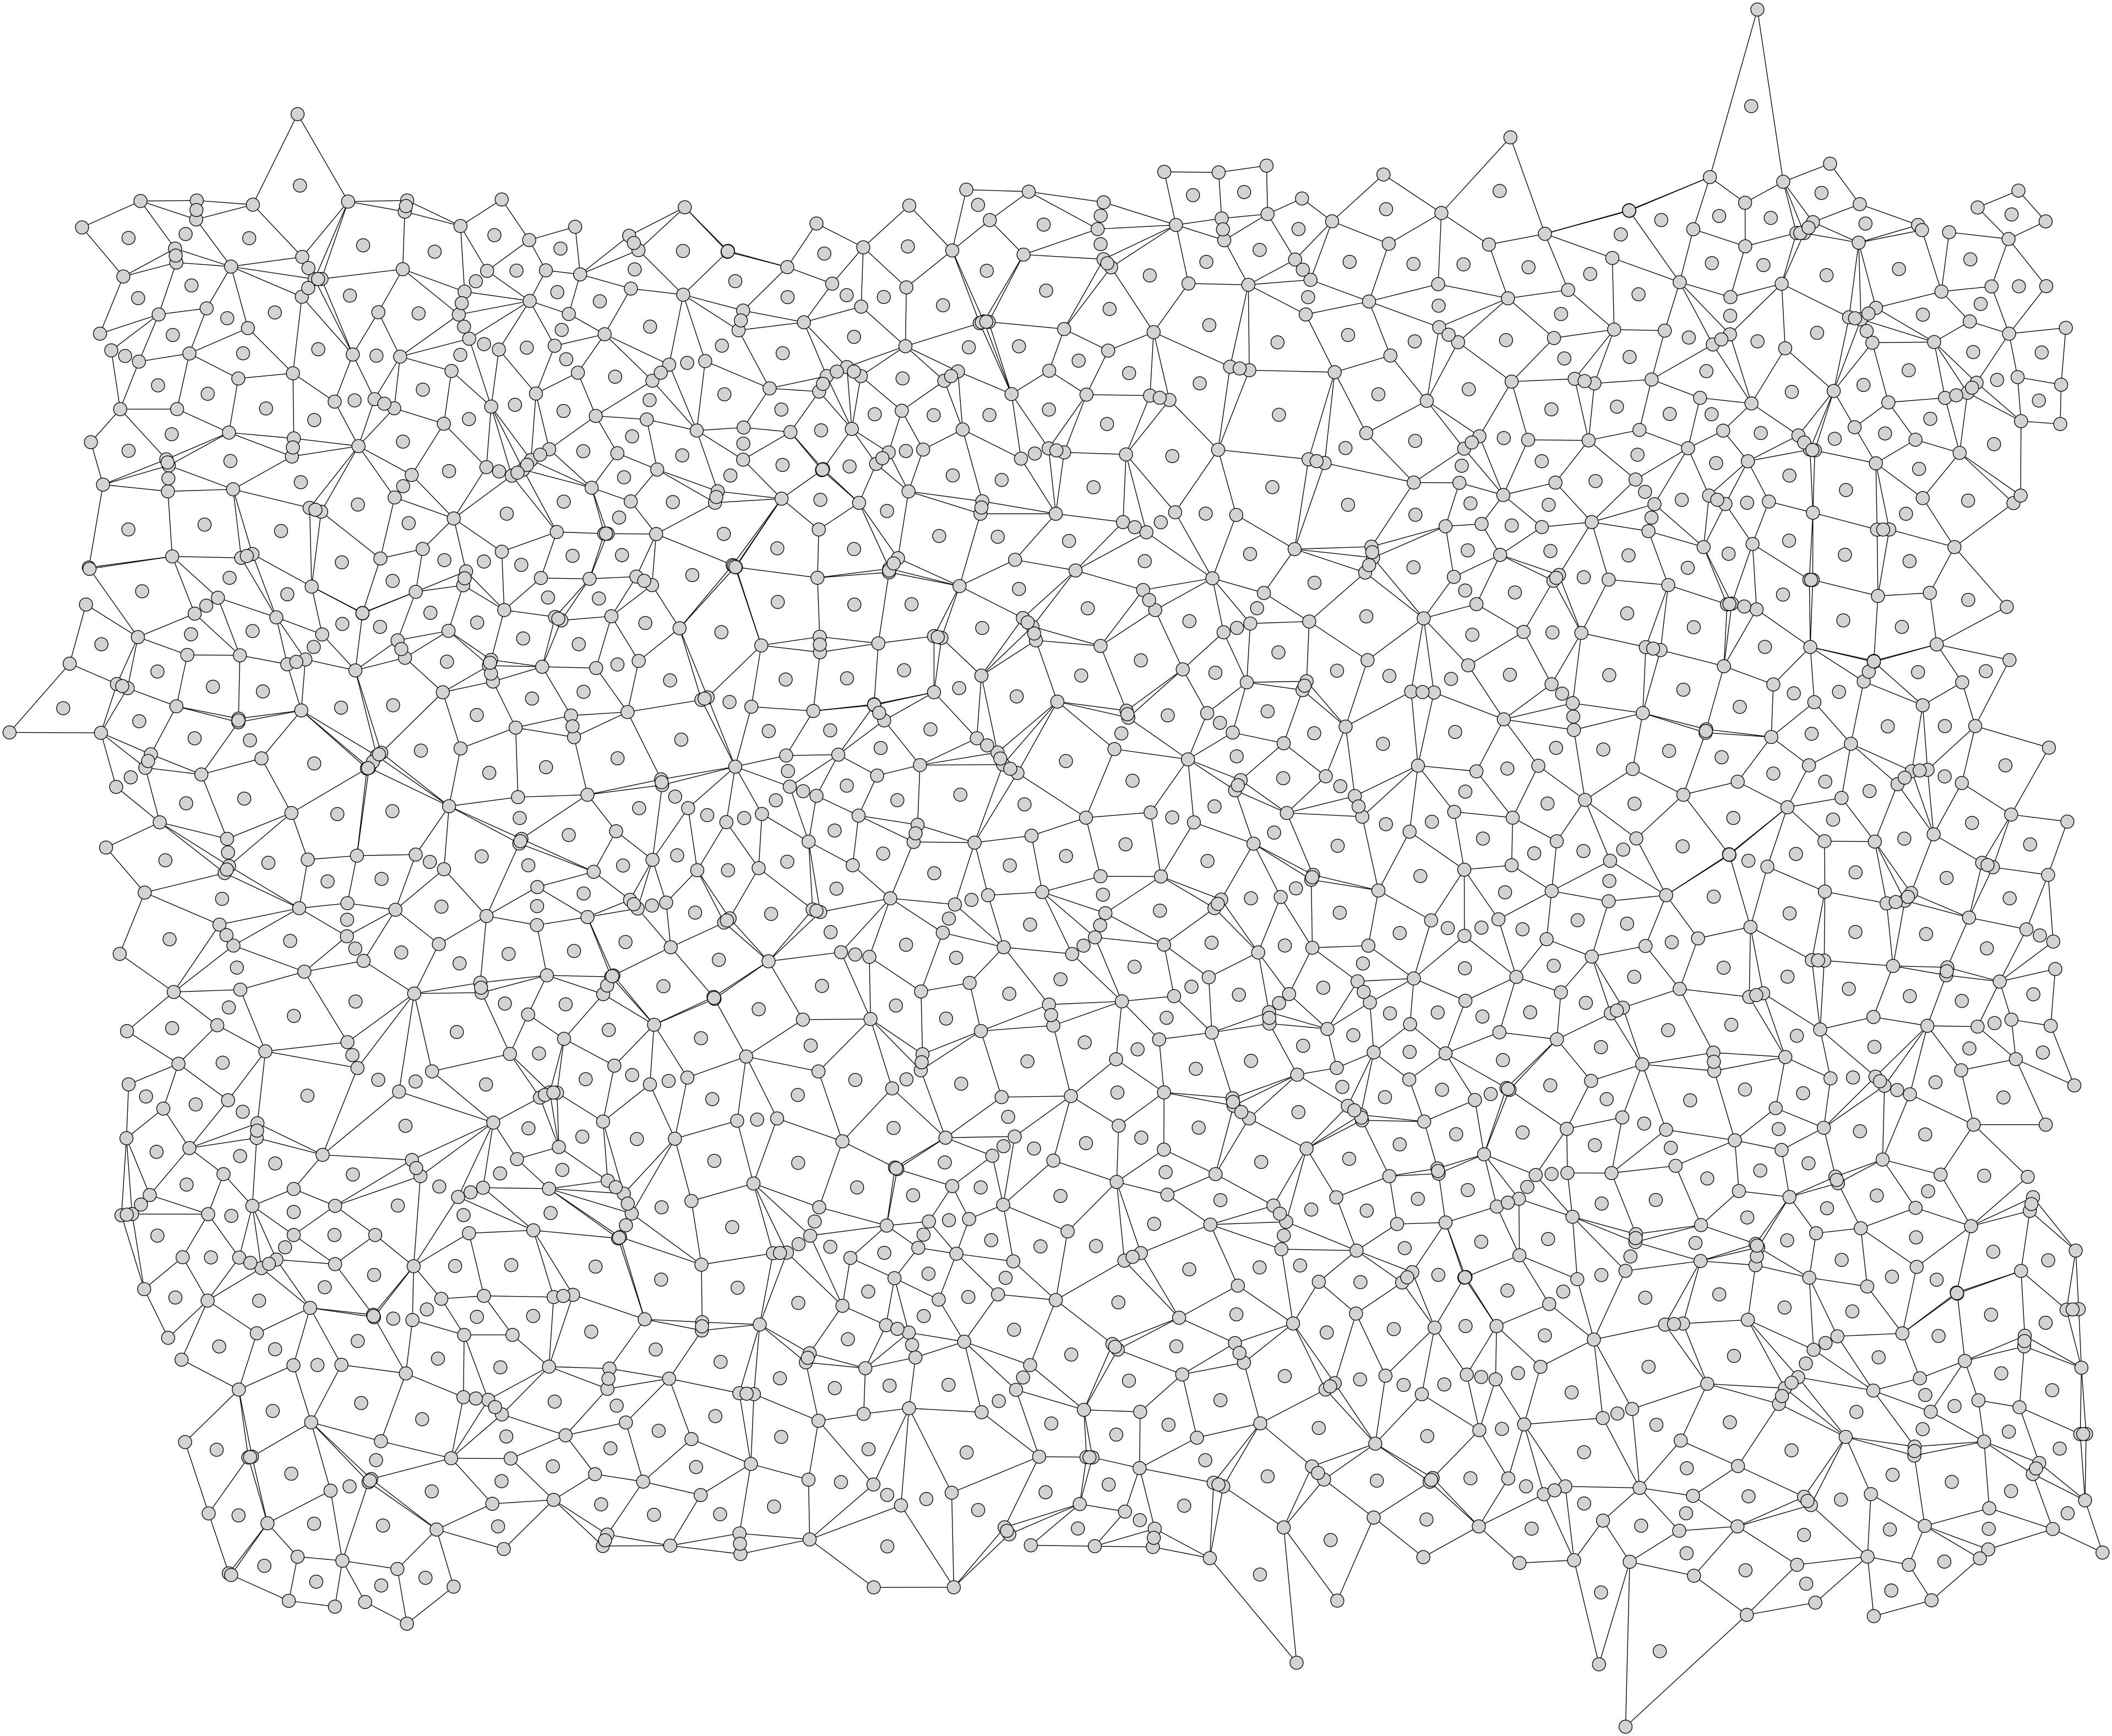
\includegraphics[width=1.0\textwidth]{ch3_figs/vquad_stoma_v2}
\caption[Voronoi Quad Grid]{
  A representative Voronoi Quad grid, generated from the same set of generator points as Figure 
  \ref{fig:voronoi_gen}.
}
\label{fig:vquad_grid}
\end{figure}

\section{Grid Degeneration}

In Chapter \ref{ch:lambda_degen}, we consider various degenerated Voronoi Quad grids
in our examination of the $\lambda$ parameter. We will discuss the methods for generating these degraded grids here.

\subsection{Generator Point Removal}
\label{subsec:gen_pt_rem}
As noted in Section \ref{subsec:vquad}, VQuad grid generation is dependent on the position of Voronoi generator points in the input Voronoi diagram. Thus, one manner of grid degeneration is simply to remove generator points from the input diagram. Since a generator point in the input diagram could be a vertex to many VQuad cells, generator point removal has the effect of taking out large chunks of the VQuad grid, as pictured in \ref{fig:genpt_degen}.

\begin{figure}[htp]
\centering
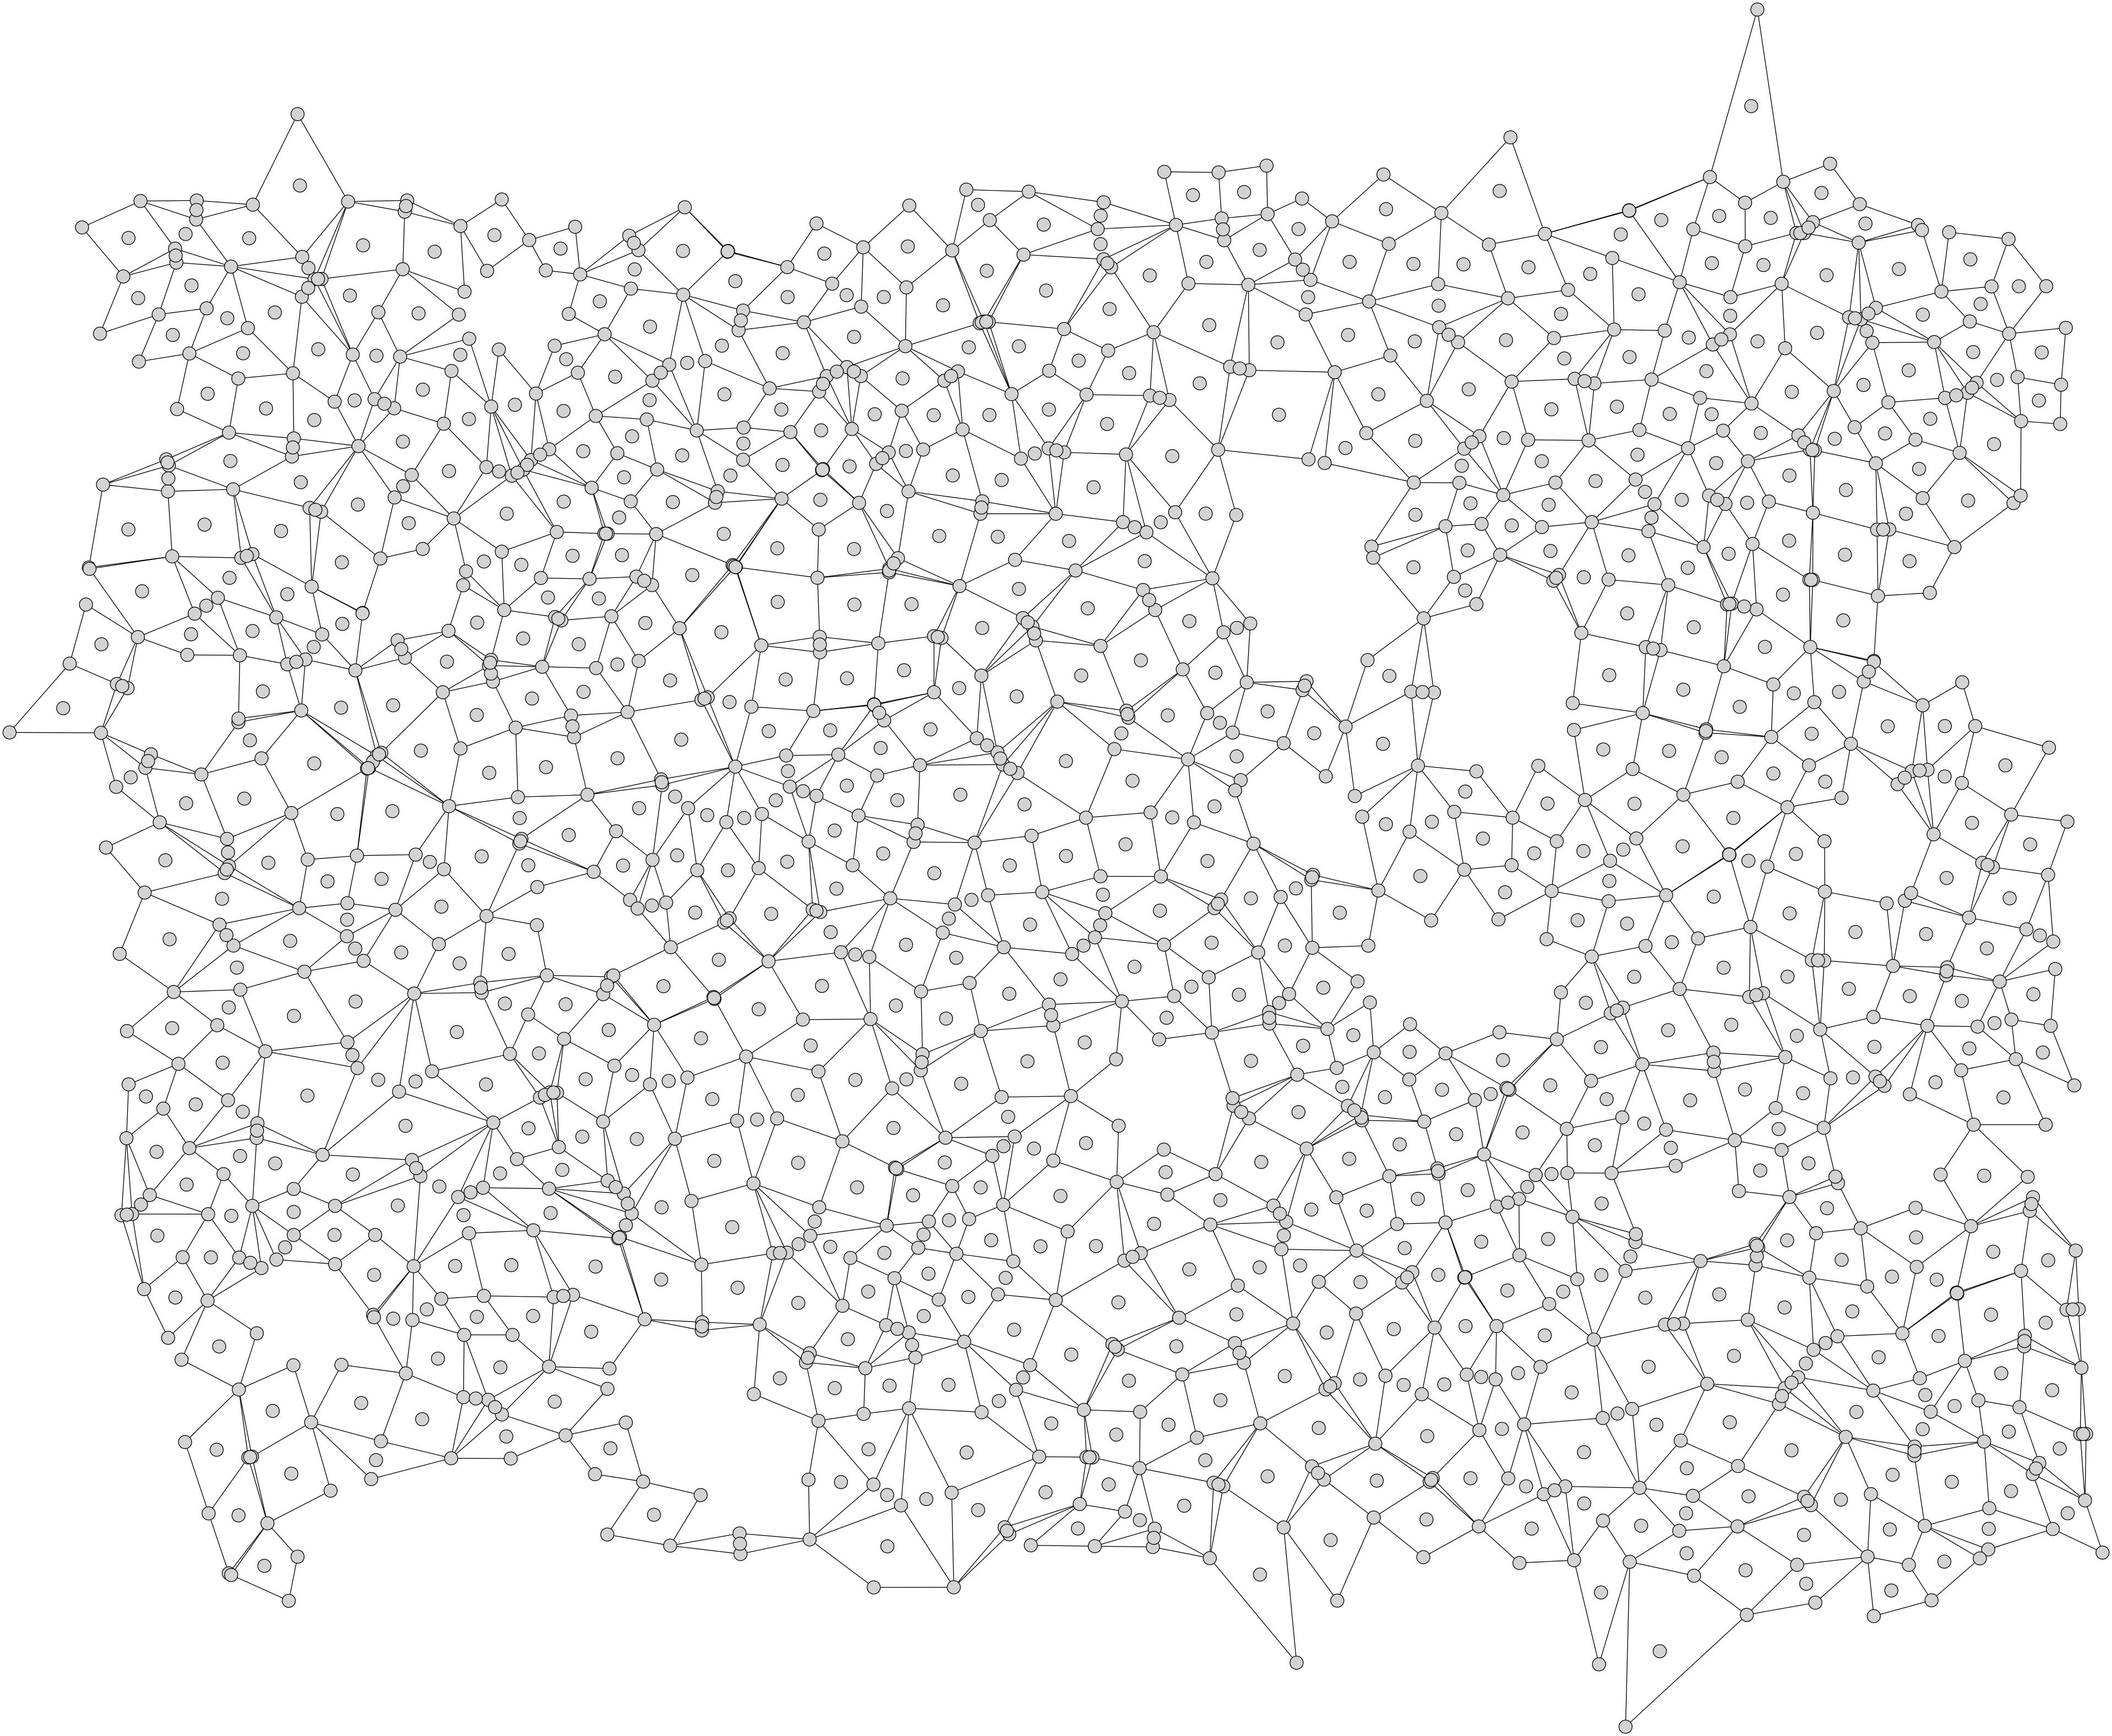
\includegraphics[width=1.0\textwidth]{ch3_figs/gen_pt_degen_7}
\caption[Generator Point Degradation]{
  A VQuad grid degraded by the removal of 7\% of the input generator points. Notice the lack of small, (particularly single cell) holes in the resulting grid.
}
\label{fig:genpt_degen}
\end{figure}

\subsection{Crosshatching Degeneration}
\label{subsec:ch_degen}
Though generator point removal provides a simple way to degrade a grid, we wanted finer-grained control over how points and edges are removed. Thus we devised a manner of degradation that allowed us to specify what local regions of the grid would be disconnected from other portions of the grid. This basic premise is to draw vertical and horizontal lines at regular width $w$ intervals apart that subdivide the irregular grid roughly into square lattice regions. Cell edges that intersect these \textit{crosshatchings} are removed from the grid with some probability $p$: cells that were formerly connected by the edge no longer are neighbors in the graph representation of the grid. Thus at $p=1.0$ we would have completely isolated ``islands'' of grid subregions. This \textit{crosshatching degeneration} technique allows us control over the degree of regional connectivity, as pictured in Figure \ref{fig:crosshatch_degen}. This manner of degradation preserves the number of cells present in the grid, instead introducing degradation by decreasing edge adjacency. Though we primarily use crosshatching degeneration as a form of edge removal, this technique also gives us a way to control generator point removal: since the crosshatchings define a square lattice partitioning of the grid, we can also choose square regions to remove with some probability $p$. Any generator points sitting within the boundary of a chosen square region will be removed from the graph. Thus we can control both the frequency of generator points removed (through adjusting $p$) as well as the average size of the of the regions removed (through adjusting $w$). This crosshatching technique allows us to parameterize the degeneration of a grid beyond simply measuring average neighborhood size.

\begin{figure}[htp]
\centering
%TODO add crosshatch degeneration figure
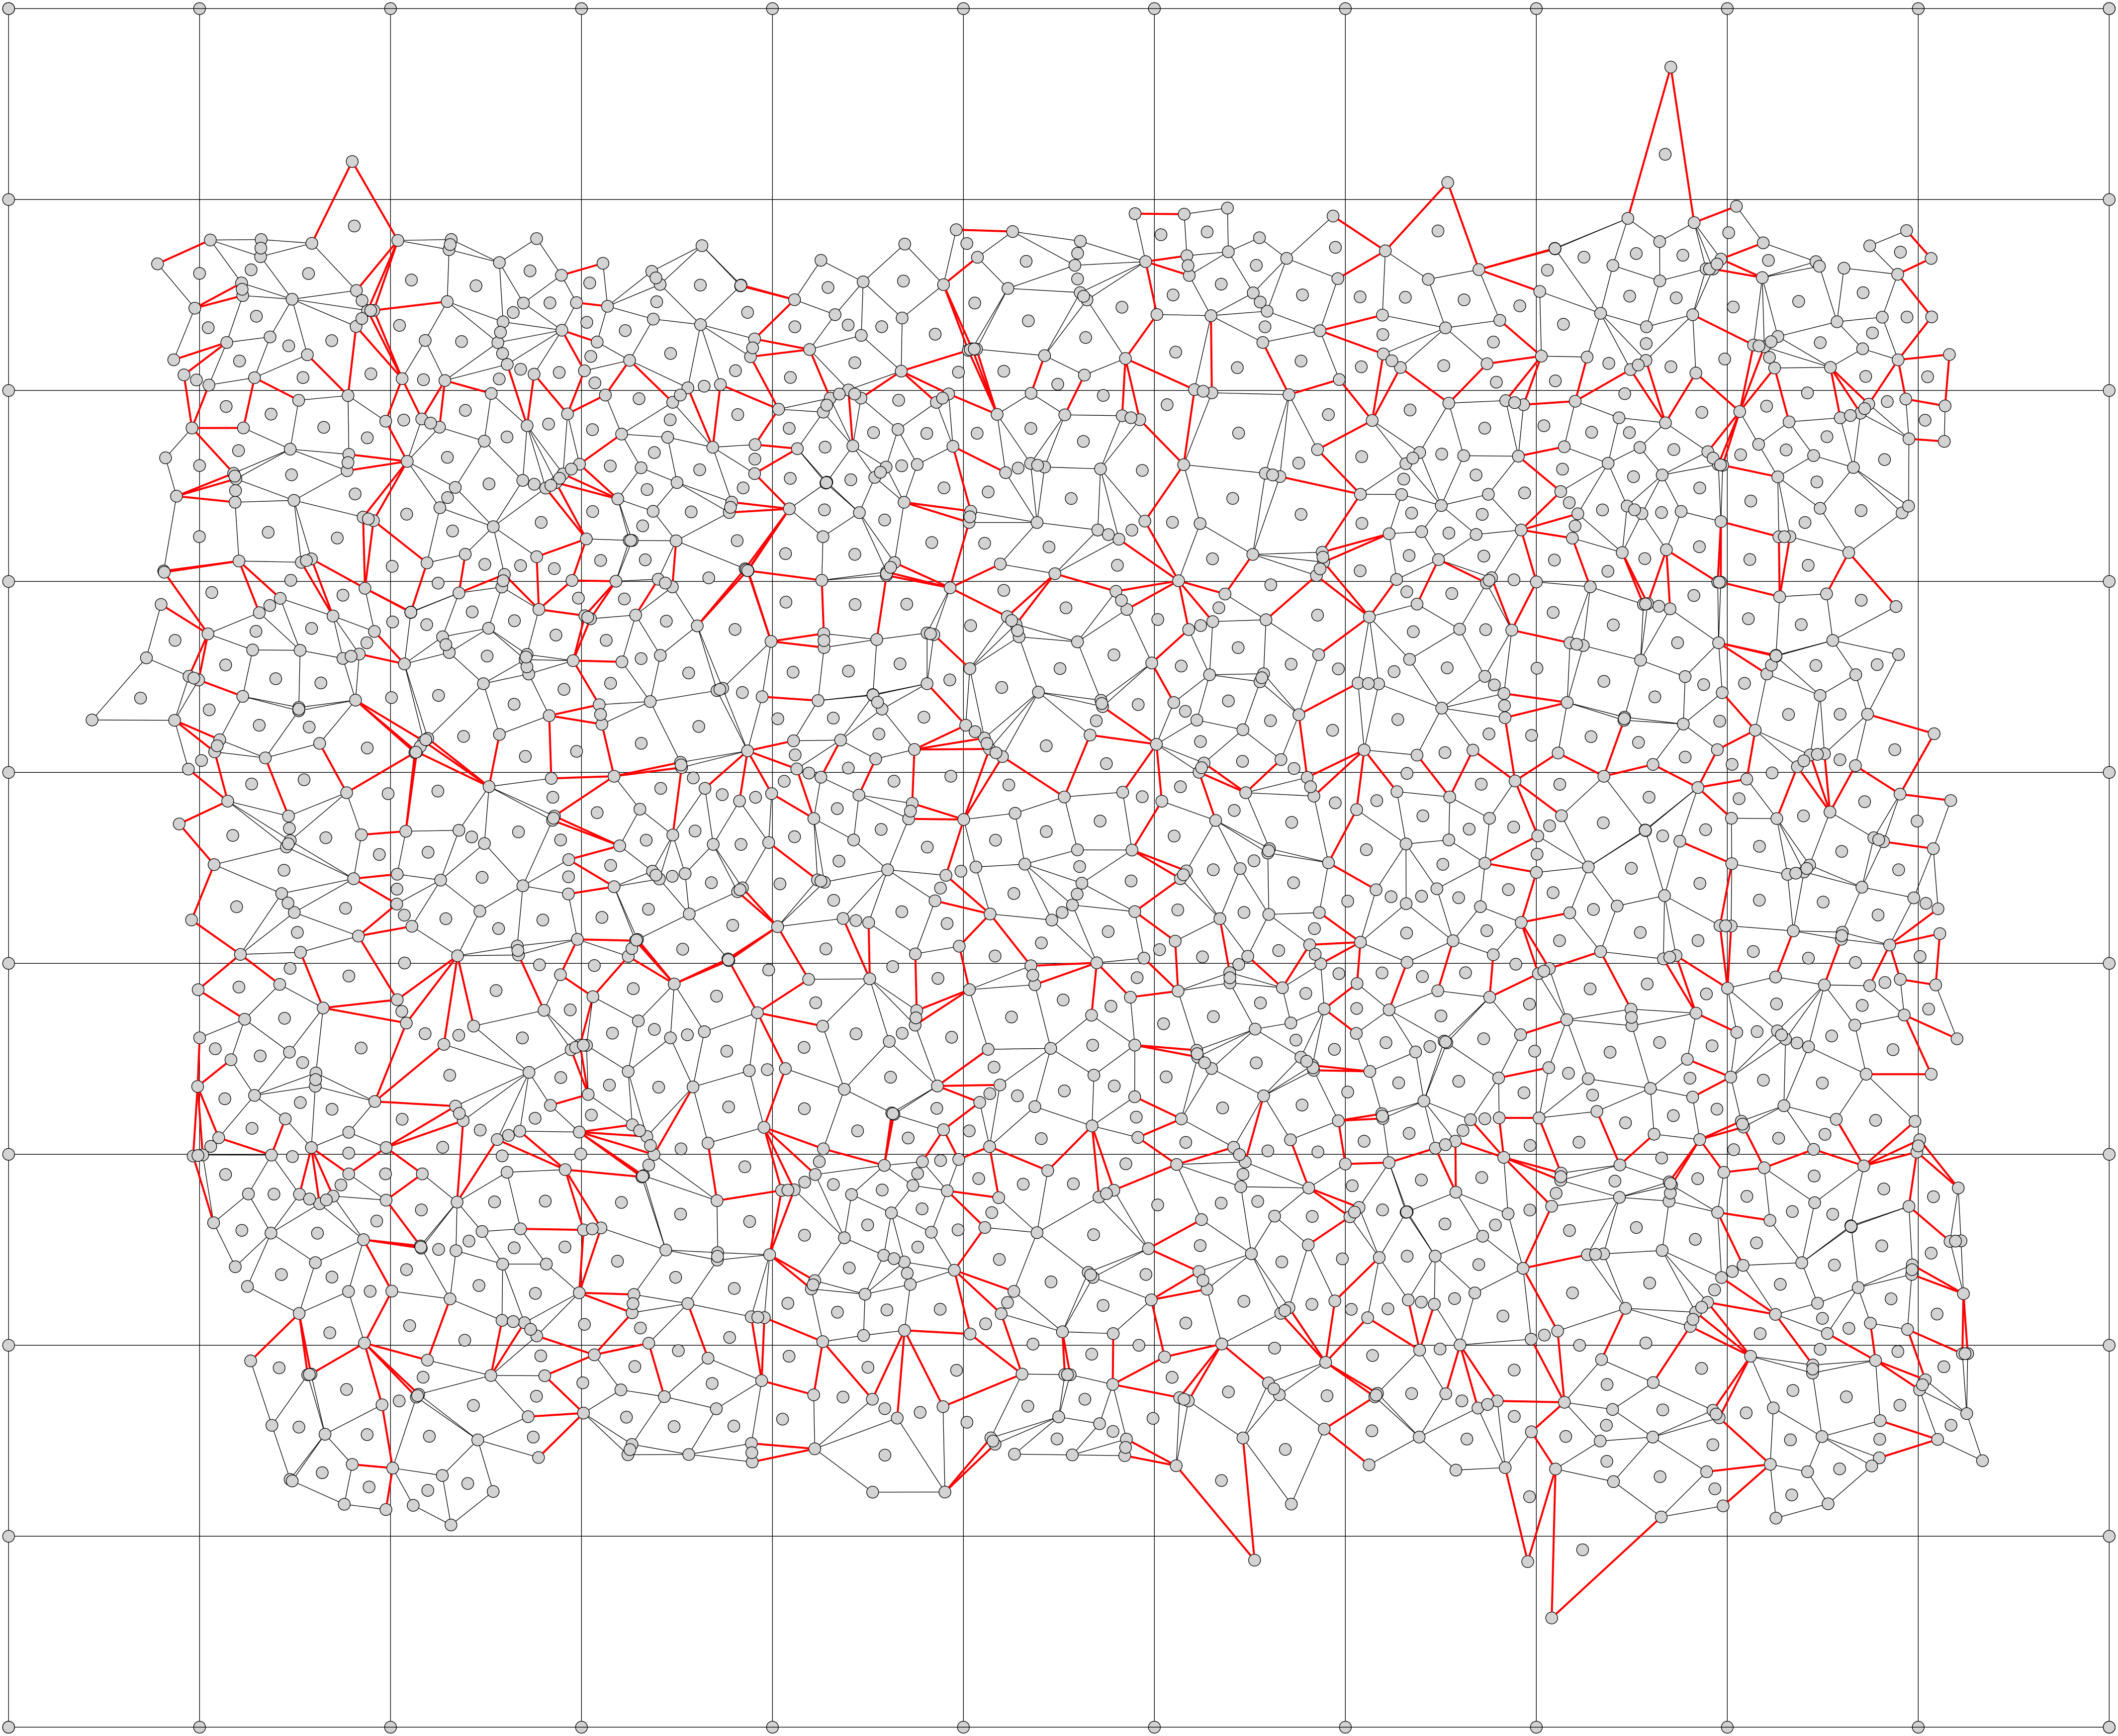
\includegraphics[width=1.0\textwidth]{ch3_figs/ch_p100_w20}
\caption[Crosshatching Degeneration]{
	An illustration of a $p=1.0$, $w=20$ crosshatch degenerated grid: edges marked in red have been removed from the connectivity graph.
}
\label{fig:crosshatch_degen}
\end{figure}

\section{Stencil and Rule Table Implementation}
\label{sec:StencilGen}
\subsection{Generalized von Neumman and Moore Neighborhoods}
We would like to maintain a notion of both von Neumman and Moore neighborhoods even on irregular grids. Thus we formally define \textit{generalized} notions of both neighborhood stencils: a \textit{generalized von Neumman neighborhood} for a cell $c$ is defined as all cells that share an edge with $c$, while a \textit{generalized Moore neighborhood} for $c$ is defined as all cells that share a vertex with $c$. These generalized neighborhood definitions are not necessarily equivalent to their standard definitions. For example, while the generalized von Neumman neighborhood for Voronoi Quad grids is identical to the regular case, the generalized Moore neighborhoods are not uniform across the grid and may have neighborhood sizes ranging from 6 to 12. Because we maintain geometry maps in our system, defining either neighborhood stencil is straightforward for any CA simulation on any grid.

\subsection{Game of Life Rule Tables}
\label{ch3:subsec_gol}
Conway's Game of Life (GoL) is a $K=2$, $N=9$ cellular automaton utilizing a Moore neighborhood stencil on regular square lattices~\cite{ga70}. Cells are either ``alive'' or ``dead'', and the rule table has traditionally been described in the following manner:

\begin{itemize}
\item Living cells stay alive if 2 or 3 neighbors are alive
\item Living cells with more than 3 living neighbors die from ``overcrowding''
\item Living cells with less than 2 living neighbors die from ``loneliness''
\item Dead cells with exactly 3 living neighbors are ``born''
\end{itemize}

However, we can also describe the GoL rules in terms of a lookup table: since there are two states, we can map a bit string of length 9 to every possible neighborhood configuration, with each position in the bit string corresponding a particular cell in the Moore neighborhood stencil (Figure~\ref{fig:gol_table}). This manner of encoding allows us to quantify and manipulate a CA's rule table, and we utilize this representation when conducting $\lambda$ experiments as described in the next section.

\begin{figure}[htp]
\centering
\begin{tabular}{| l | l |}
\hline
Neighborhood & Output \\
\hline
00000011\textbf{1} & 1 \\
\hline
11000110\textbf{1} & 0 \\
\hline
00001000\textbf{1} & 0 \\
\hline
00101010\textbf{0} & 1 \\
\hline
\end{tabular}
\caption[Game of Life Rule Table]{
	A few representative entries in the Game of Life Rule Table (there are $2^9$ entries in total). The center cell is the rightmost bit, in bold. These table entries correspond exactly to the four Game of Life rules as described in Chapter~\ref{ch3:subsec_gol}.
}
\label{fig:gol_table}
\end{figure}

\subsection{$\lambda$ Rule Tables}
\label{subsec:ch3_lamb}
%wolfram command is: rotations with 4 beads, 8 colors
%TODO Burnside's lemma?
In the $\lambda$ experiments performed by \citeauthor{wo90}, rule tables must be \textit{isotropic} in that all planar rotations of a particular neighborhood configuration map to the same output cell state; this condition removes the global property of spatial orientation from influencing rule transitions~\cite{av00,wo90}. As a result, what would be a $K^N$ sized table results in a smaller table because only rotationally distinct neighborhood configurations are unique entries: specifically, if we consider the $K=8$, $N=5$ case the rule table of size $8^5 = 32,768$ is reduced to a rule table of size $8,352$ (see Appendix \ref{appB:rot} for calculation). To generate these tables, we iterate over all $K^N$ possible neighborhood values, canonicalize their string representations by finding their \textit{lexicographically minimal rotation}, and track only the unique neighborhoods. For example, in the $K=8, N=5$ case, neighborhoods ``0110'' and ``1001'' map to the same minimal rotation neighborhood of ``0011''. We then append a center state value to the end of this canonical neighborhood representation, thus creating the keys for our $\lambda$ rule table mapping with the output state for that particular neighborhood configuration as the value.

Rule tables must also be \textit{strongly quiescent} in that a neighborhood configuration that consists entirely of the quiescent state must map to the quiescent state. This condition is satisfied by simply initializing the appropriate entry in the transition table and then ensuring that entry is not modified throughout a given experiment run.

\section{Summary}
We have built a CA simulation system that is modular and extensible. The system performs sufficiently to run a gamut of CA experiments within a reasonable amount of time. The system is also flexible enough so that we can make changes to any portion of the system through implementing various derived classes, and the command line interface allows us to easily tweak experiment parameters without having to change the source code.

\processdelayedfloats

\chapter{Penrose Life Experiments}
\label{ch:penrose}

We begin our exploration of irregular CA by considering aperiodic tilings. Specifically, we build upon work done by \citeauthor{hi05} (see Chapter \ref{subsec:gol}) in examining the Game of Life on Penrose Tilings (\textit{Penrose Life}). Aperiodicity is a move away from the regularity found in square lattices but still maintains some local neighborhood structure. 
%(TODO more explanation of the link between aperiodic and irregularity, insert neighborhood figure from Owen/Stepney?). 
One of our goals is to investigate the potential for information transfer across an irregular CA space. In the case of Game of Life, moving particles named \textit{gliders} are the most basic representation of information transfer across a regular grid. However, these gliders exploit the regularity of the grid in their movement and as a result are not robust to changes in their immediate environment: over 99\% of possible environment configurations a glider can encounter will be destructive to it~\cite{be14}. Thus we imagine that information transfer may be more difficult to achieve on grids that do not maintain spatial consistency. These Penrose Life investigations explore the possibility of moving particles in a CA grid that relaxes some of the regularity found in standard square lattices.     

Another goal is to investigate CA behavior at the boundary of the grid. Typical CA simulations assume toroidal boundaries that produce an ``infinite'' grid wrapping around on itself, but natural dynamic systems are unlikely to have this property. Finite spaces will inevitably have boundaries and complex CA must be able to handle these unique conditions where the neighborhood for a cell on the boundary is incomplete. Since toroidal boundary conditions are impossible for an aperiodic tiling, we will examine potential boundary interactions in Penrose Life.

%TODO change section title?
%\section{Replication and Extension of \citeauthor{hi05}'s Work}

\citeauthor{hi05} ran experiments on Kite/Dart Penrose tilings investigating random initial starting configurations (\textit{soups}) and the resulting stable structures left on the grid (\textit{ash}). \citeauthor{ow10} continued this work on Thin/Thick Rhombus Penrose tilings and also examined repeating periodic structures (\textit{oscillators}) in Penrose Life. We replicate and extend their work here as well.

%TODO add figures 
\iffalse
\begin{figure}[htp]
\centering
\begin{subfigure}[t]{0.4\textwidth}
	\centering
	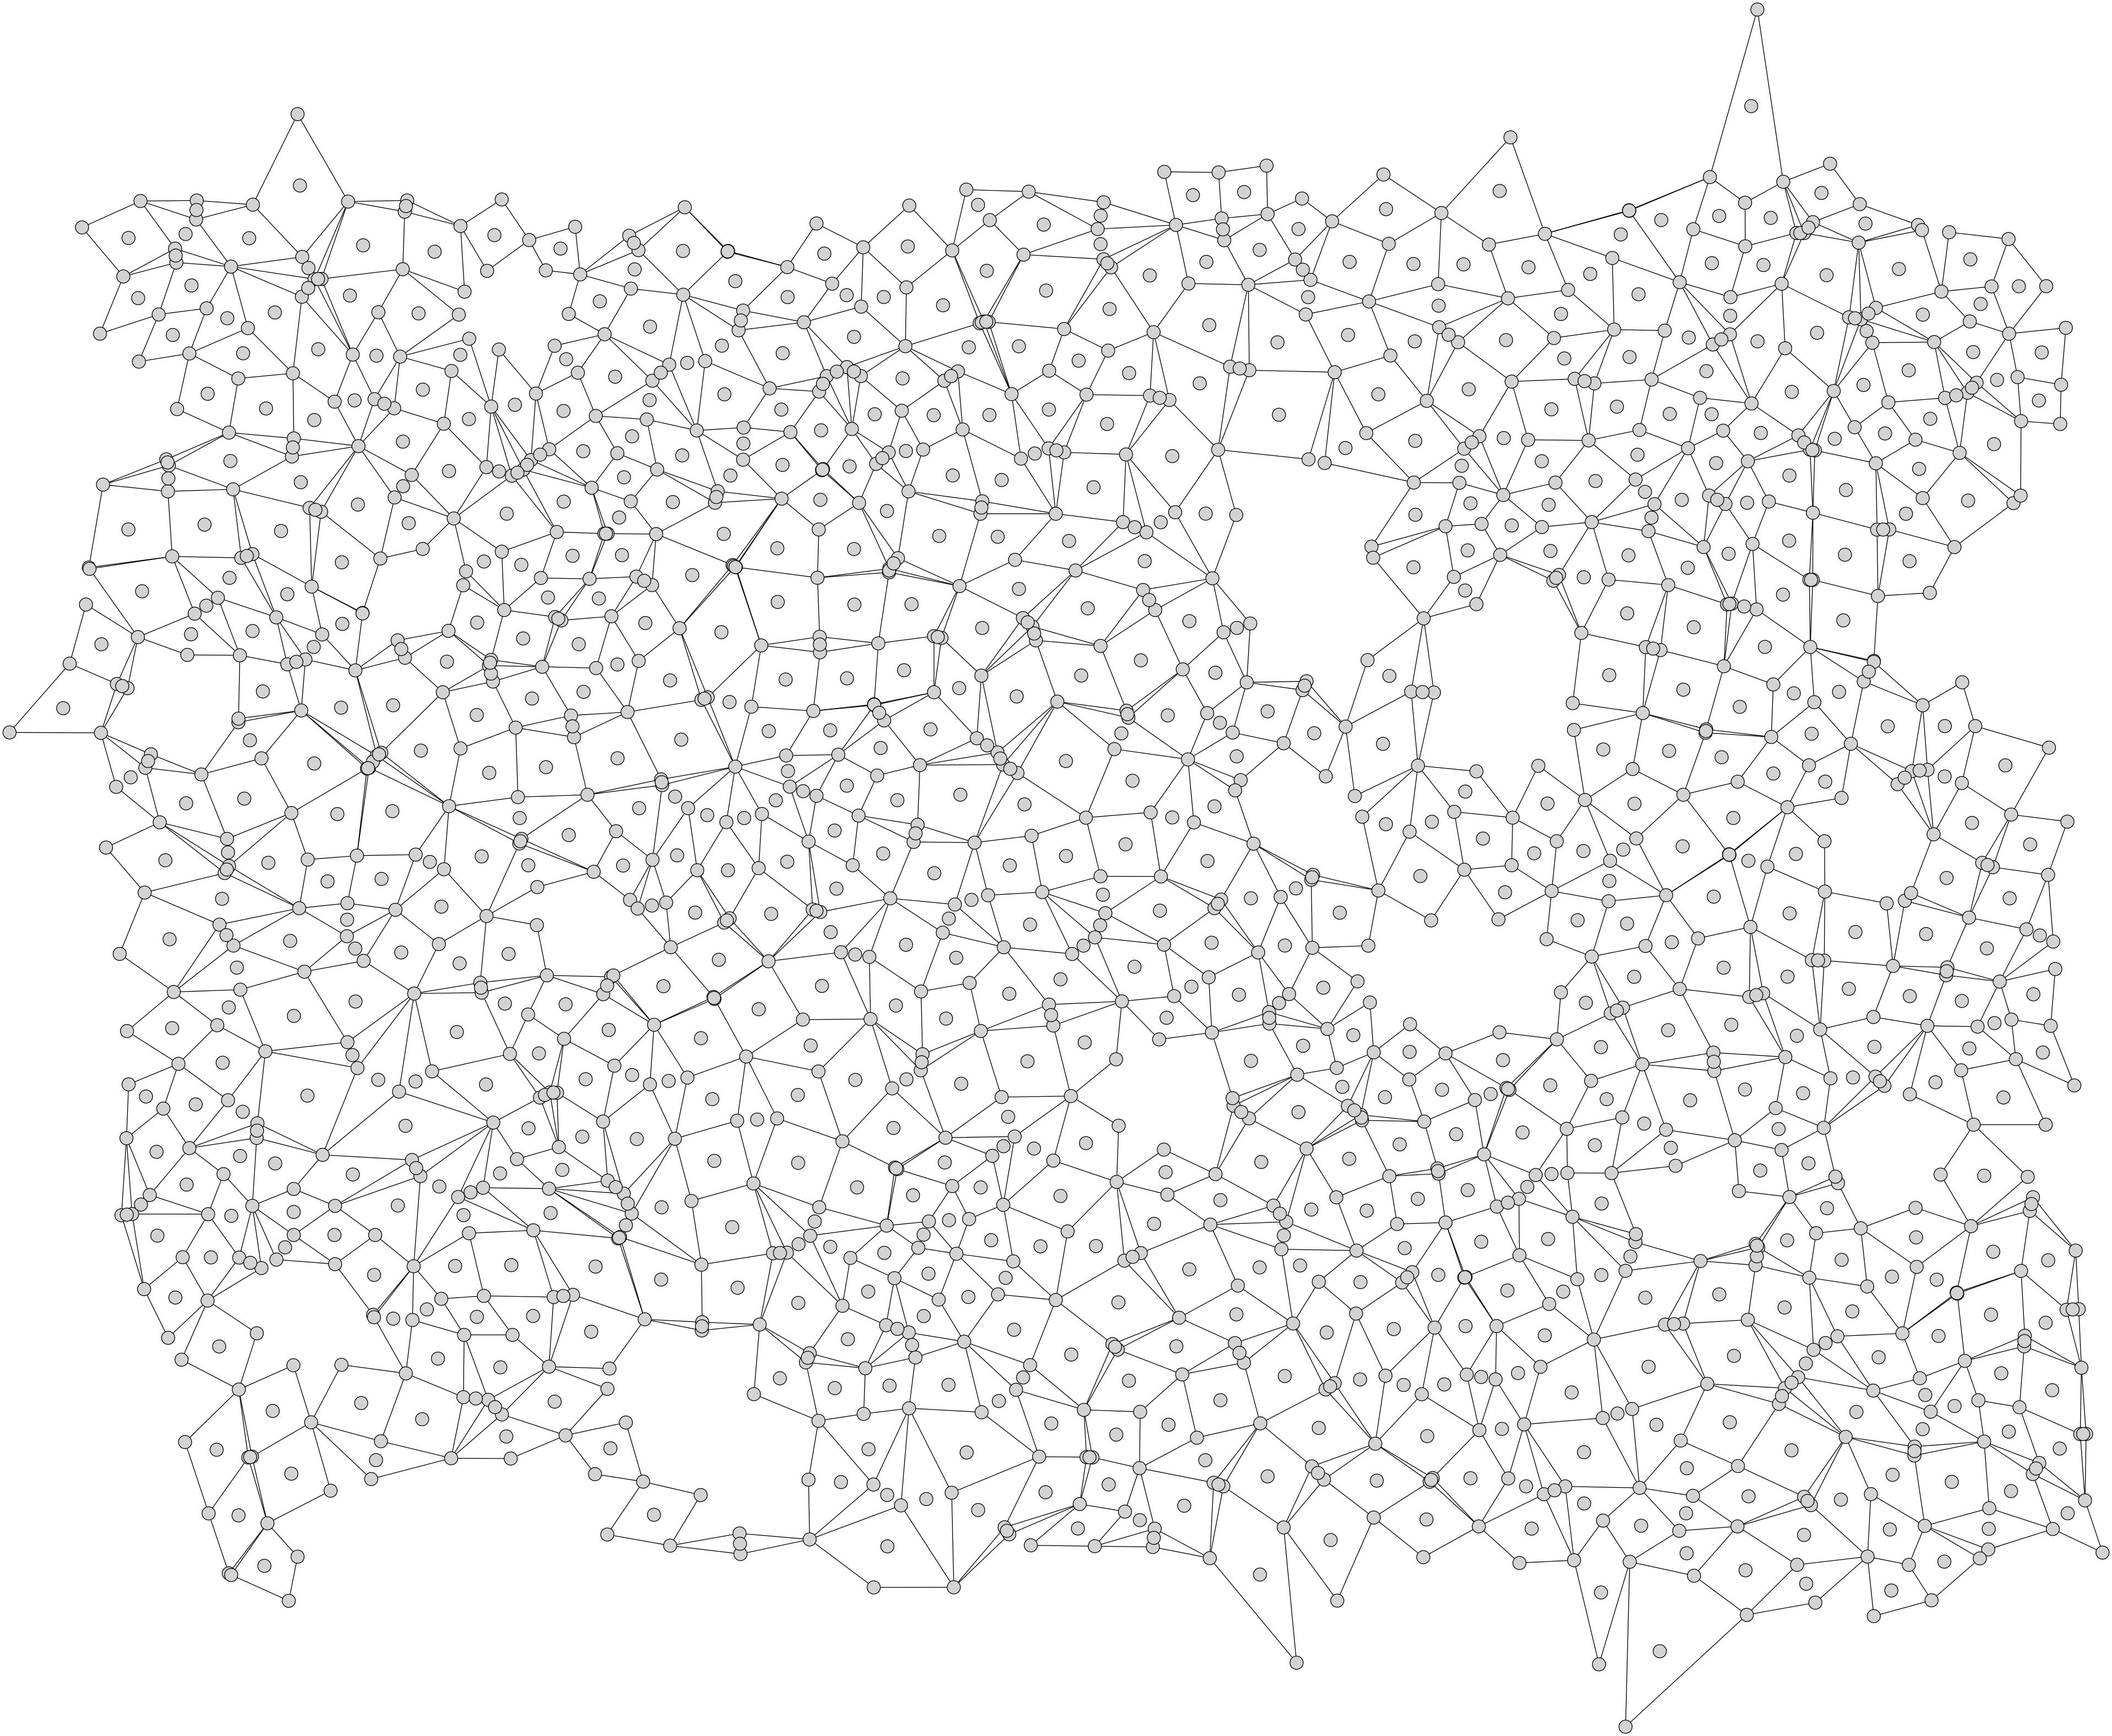
\includegraphics[width=\textwidth]{ch3_figs/gen_pt_degen_7}
	\caption{Kite/Dart Penrose Tiles}
	\label{fig:penrose_types:kd}
\end{subfigure}
~
\begin{subfigure}[t]{0.4\textwidth}
	\centering
	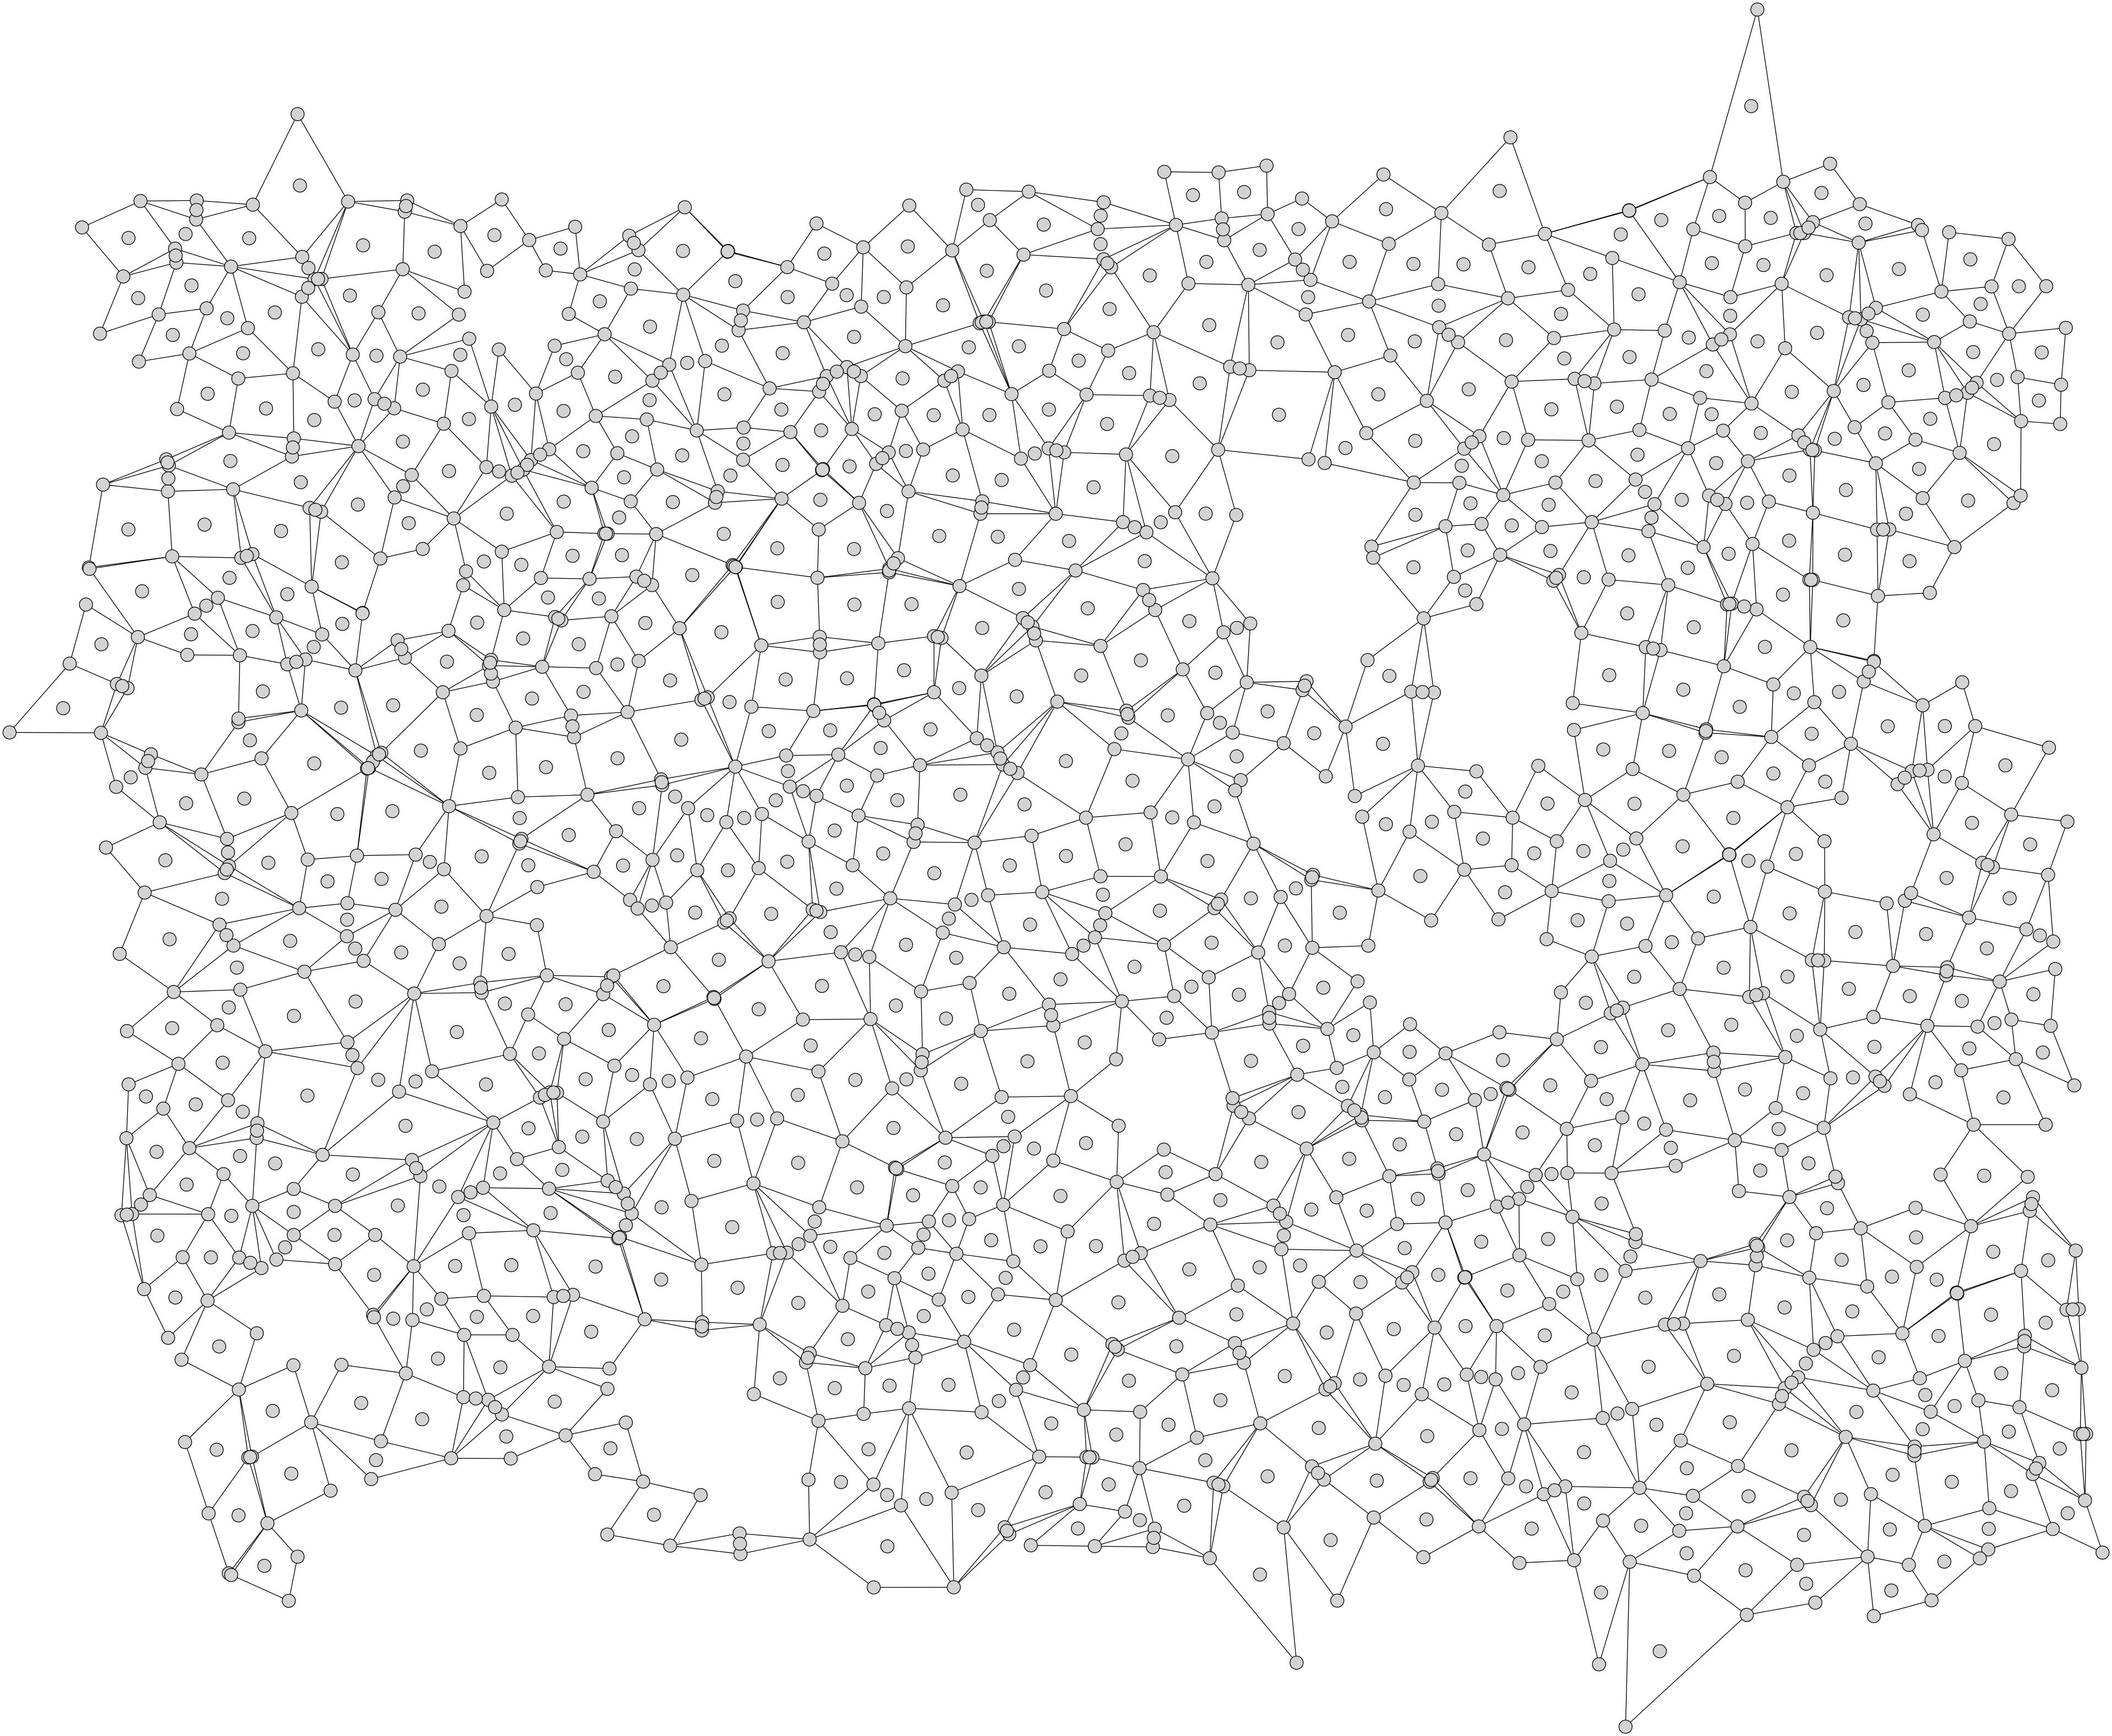
\includegraphics[width=\textwidth]{ch3_figs/gen_pt_degen_7}
	\caption{Thin/Thick Rhomb Tiles}
	\label{fig:penrose_types:tt}
\end{subfigure}

\caption[Penrose Tile Types]{
	An illustration of two common Penrose Tilings: Kites/Darts and Thin/Thick Rhombs.
}

\end{figure}
\fi


\begin{figure}[htp]
\centering
\begin{subfigure}[t]{0.6\textwidth}
	\centering
	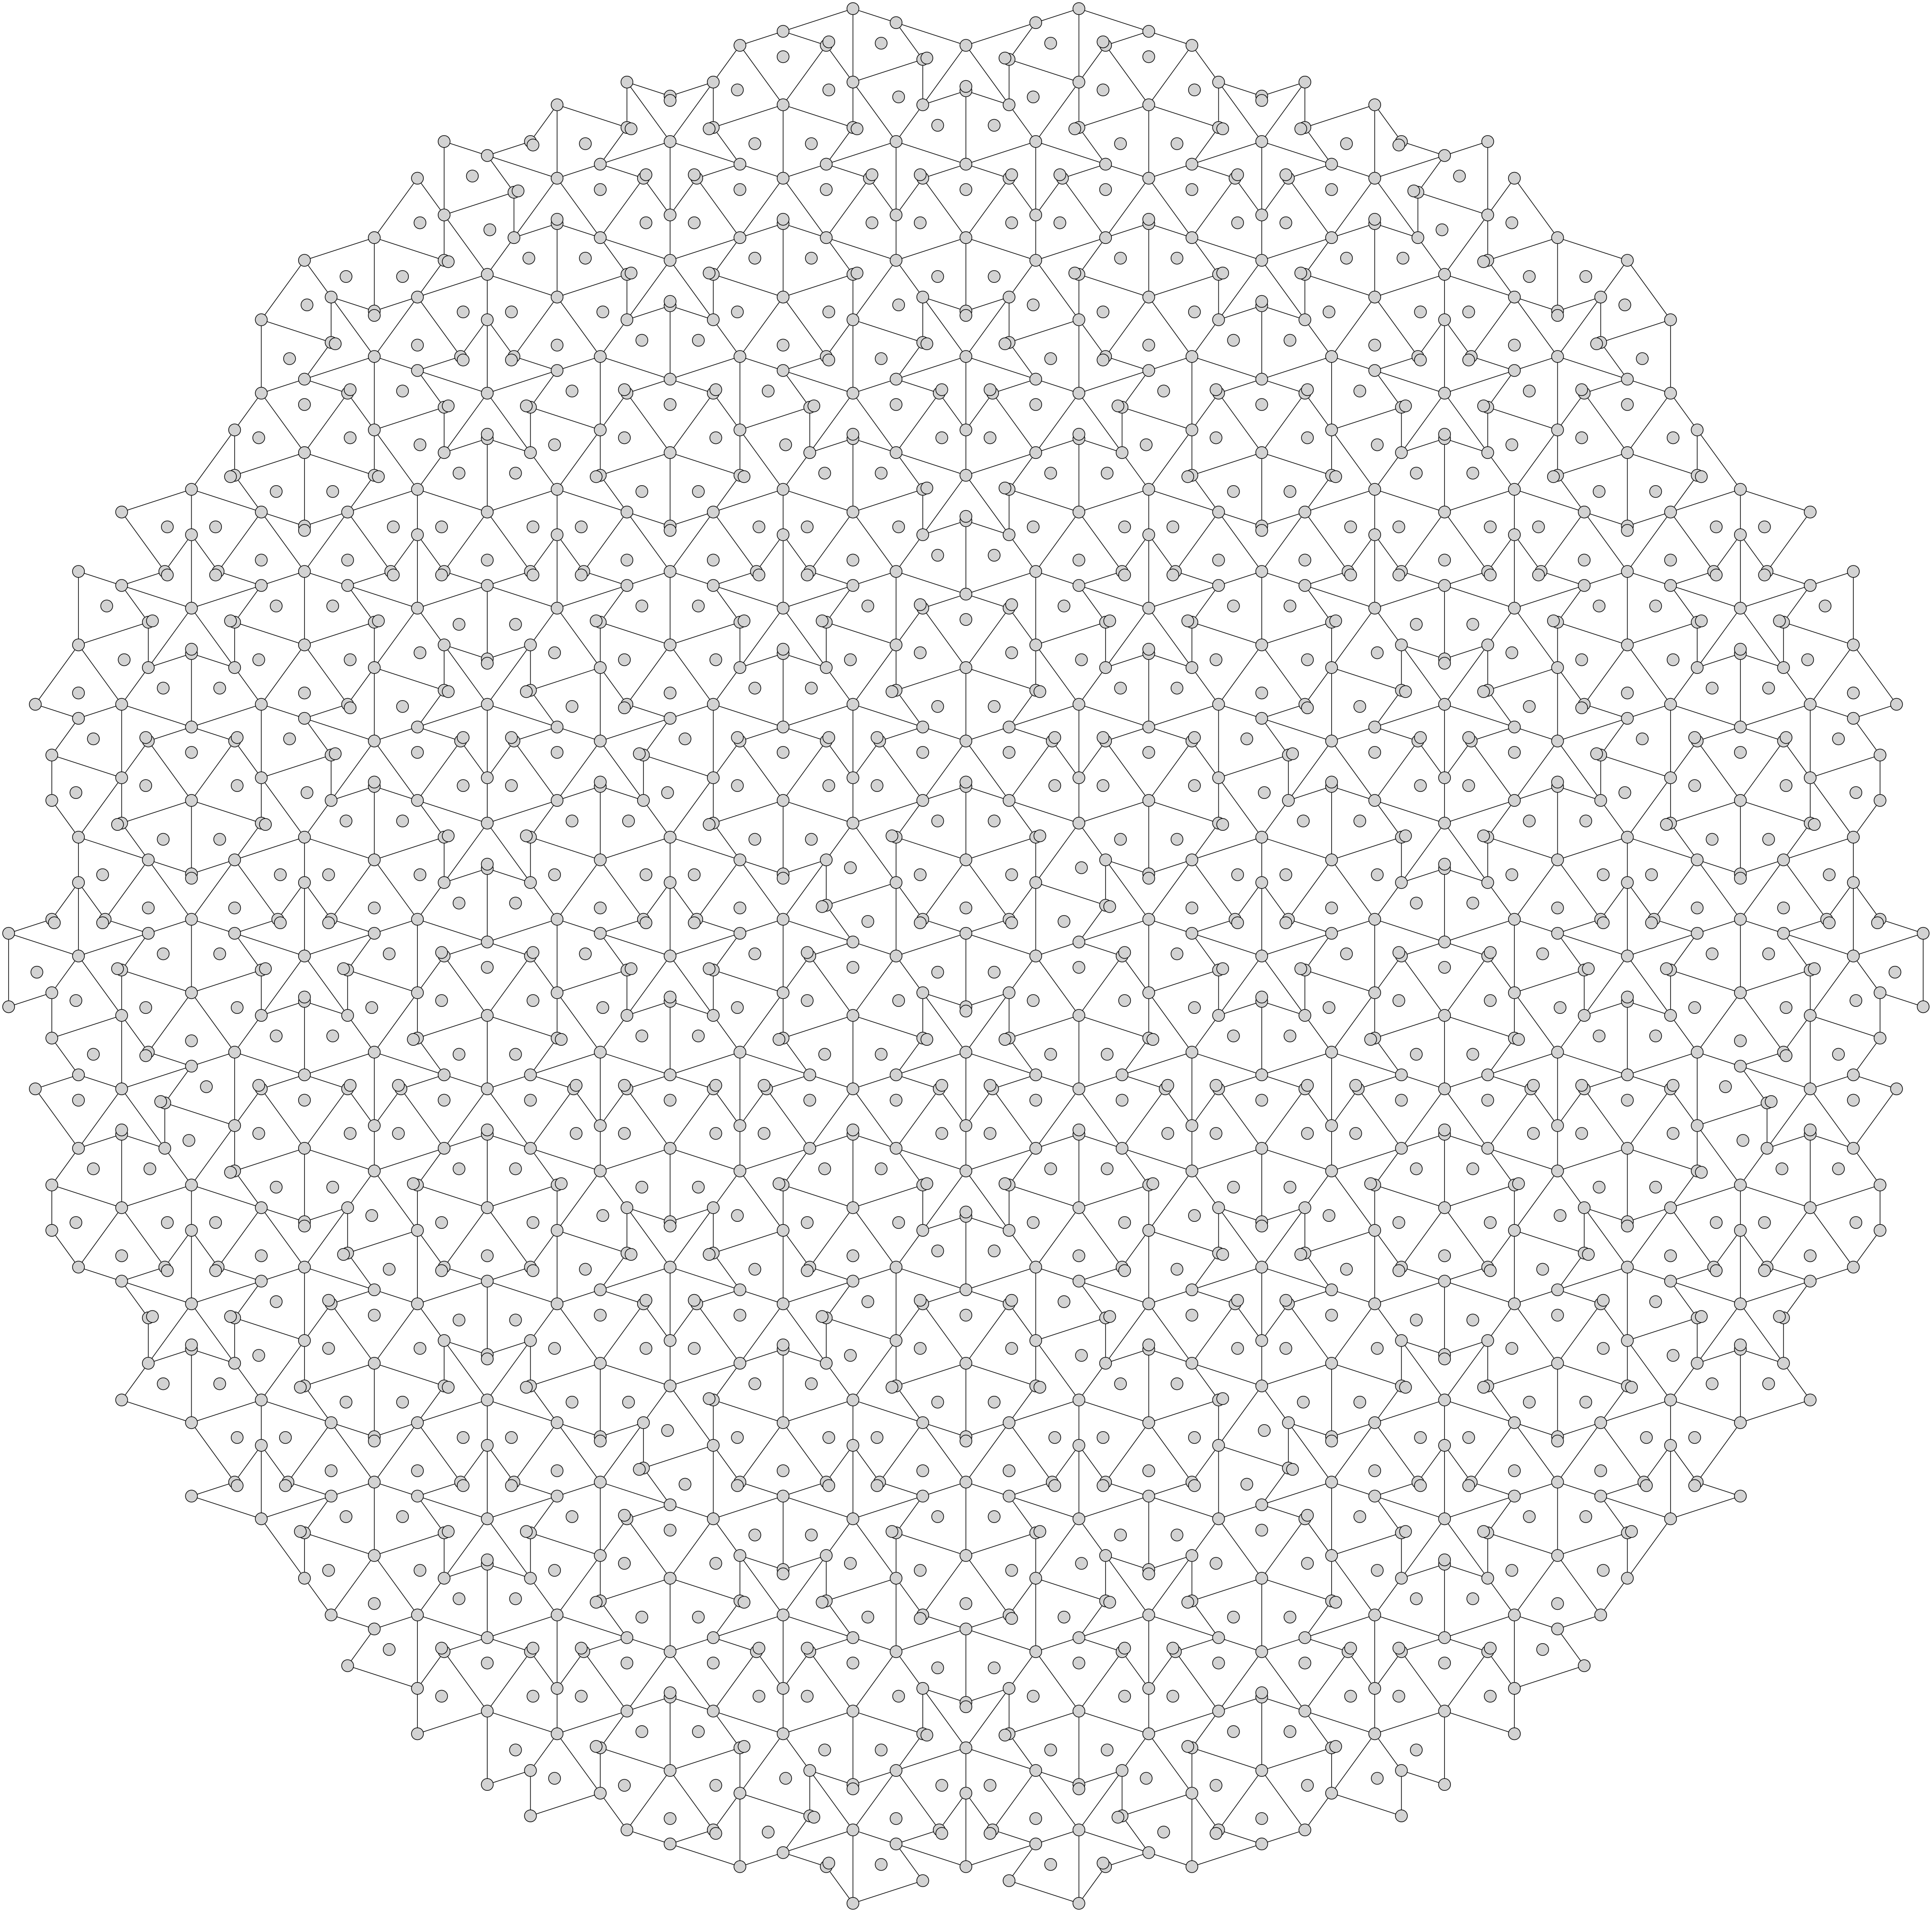
\includegraphics[width=\textwidth]{ch4_figs/ckd}
	\caption{Circular Kite/Dart Grid}
	\label{fig:kd_circ}
\end{subfigure}
~
\begin{subfigure}[t]{0.6\textwidth}
	\centering
	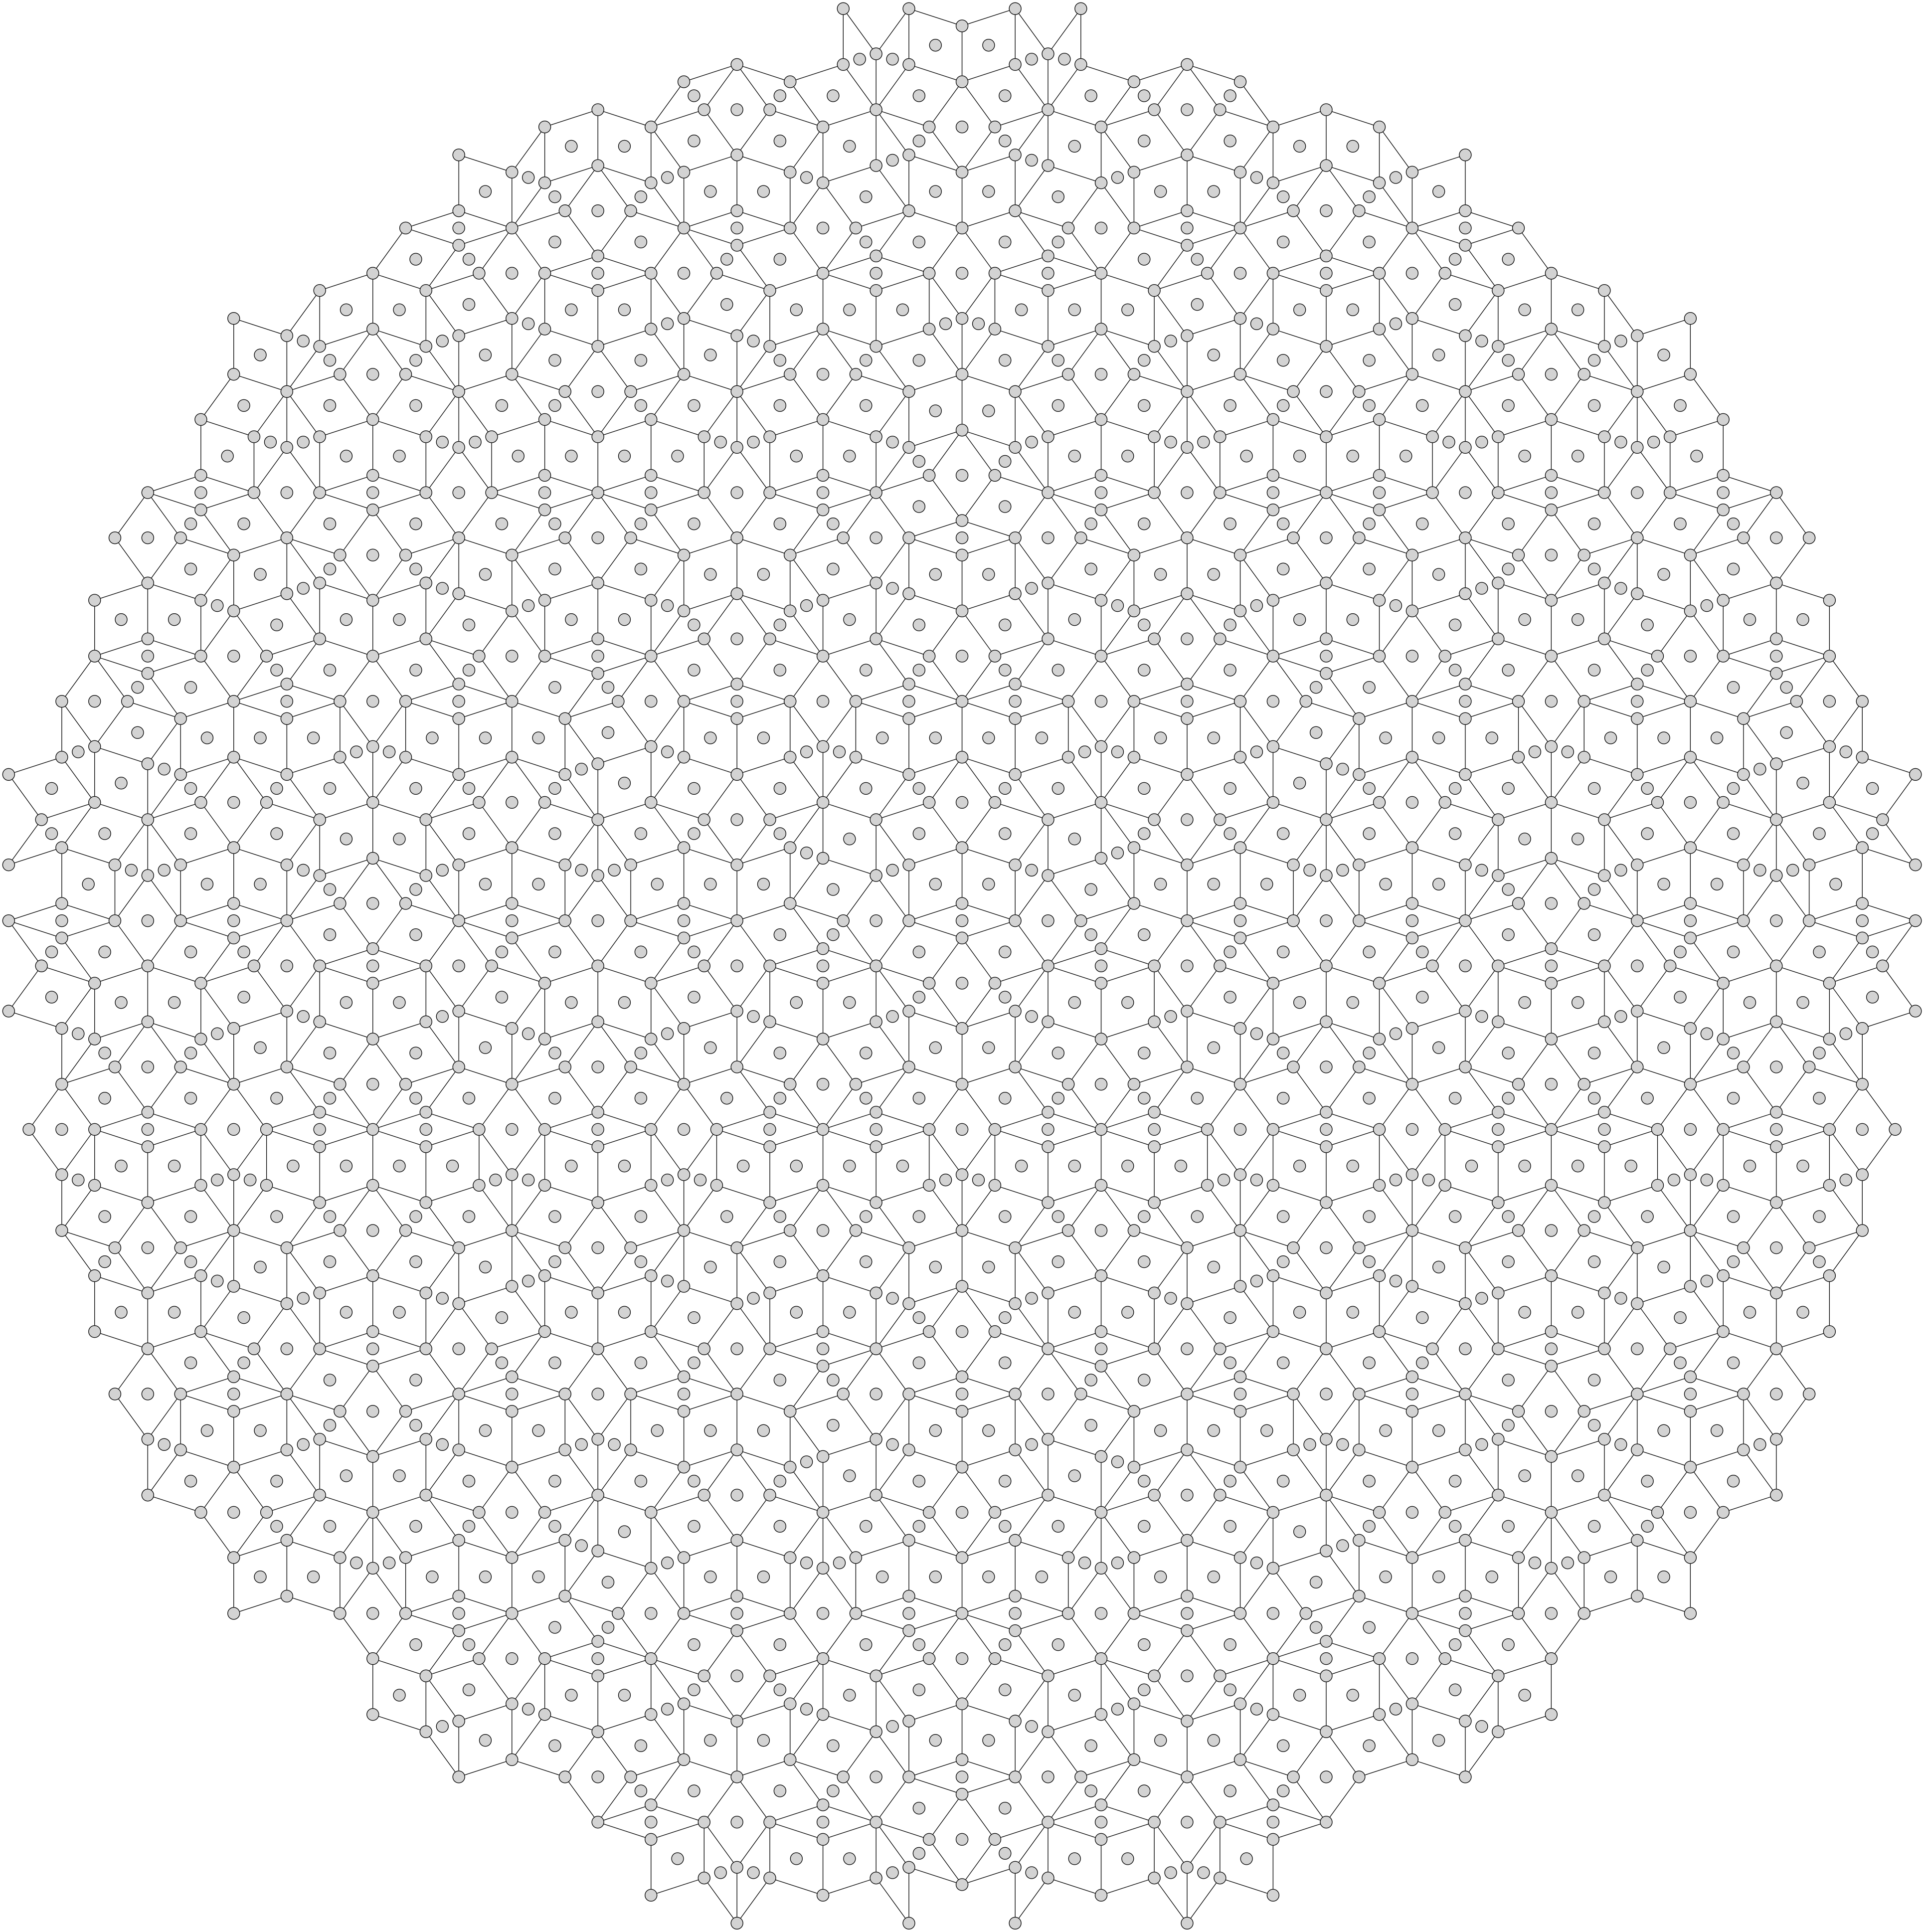
\includegraphics[width=\textwidth]{ch4_figs/crh}
	\caption{Circular Rhomb Grid}
	\label{fig:tt_circ}
\end{subfigure}

\caption[Circular Penrose Tilings]{
	An illustration of the two circular Penrose tilings we utilize in our baseline ash density and lifetime to stability experiments.
}
\label{fig:penrose_circ}
\end{figure}

\section{Lifetime to Stability and Ash Density}
\label{ch4:lifetime}
In order to locate where interesting behavior may occur in Penrose Life, we begin by examining the full range of \textit{initial soup densities} (percentage of ON cells in the starting configuration) from $d=0.01$ to $d=0.99$, measuring both \textit{lifetime to stability} (the number of timesteps a given configuration takes to stabilize) and final \textit{ash density} (the percentage of the grid in a stable state).

\subsection*{Experimental Setup}
Both Kite/Dart and Thin/Thick Rhomb Penrose tilings are considered. We utilize circular grids, with the Kite/Dart grid containing 995 cells and Rhomb grid containing 1,075 cells. The Rule Table utilizes standard Game of Life rules with generalized Moore neighborhood stencils. For each initial soup density we run 100 trials and average our statistics across all the trials, resulting in 9,900 CA simulations which. The tilings are pictured in Figure \ref{fig:penrose_circ}.

\subsection*{Results}
Lifetime to Stability and Ash Density graphs for Kites/Darts are pictured in Figure \ref{fig:ckd_lifetime_density}. These results agree with the data presented by \citeauthor{hi05} shown in Figure \ref{fig:hi05_lifetime_density}, with our circular tiling falling in between the S and M grids in terms of size: both lifetime graphs have a right-skewed distribution while the ash density plots show little correlation between lifetime and final ash density for initial soup densities of $d=0.20, 0.40, 0.60$. The ash densities fall within a range of about $d=0.00$ to $d=0.03$. It's important to note that though the lifetime graphs have the same distribution shape as the standard Game of Life lifetime graph, the average lifetimes for the Penrose tilings are much lower than the standard grid (Figure \ref{fig:hi05_reg_lifetime}). Similarly, though the ash density plots for the standard grid show no correlation between lifetime and ash density like the Kite/Dart plot (Figure \ref{fig:hi05_reg_density}), the final ash densities fall in a higher range of about $d=0.02$ to $d=0.06$. These results suggests that the overall qualitative behavior of Penrose Life could be similar to the standard Game of Life but also shows that it is much more difficult to maintain coherent Life structures on irregular grids.

\begin{figure}[htp]
\centering
\begin{subfigure}[t]{0.6\textwidth}
	\centering
	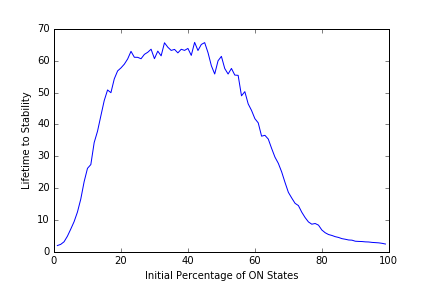
\includegraphics[width=\textwidth]{ch4_figs/ckd_lifetime}
	\caption{Kite/Dart Lifetime to Stability Graph}
\end{subfigure}
~
\begin{subfigure}[t]{0.6\textwidth}
	\centering
	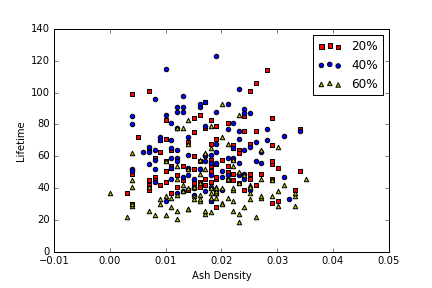
\includegraphics[width=\textwidth]{ch4_figs/ckd_ash_density}
	\caption{Kite/Dart Ash Density Scatter Plot}
\end{subfigure}

\caption[Kite/Dart Lifetime and Ash Density Graphs]{
	Lifetime to Stability and Ash Density graphs for the Kite/Dart circular tiling, grid size = 995. 
}
\label{fig:ckd_lifetime_density}
\end{figure}

\begin{figure}[htp]
\centering
\begin{subfigure}[t]{0.6\textwidth}
	\centering
	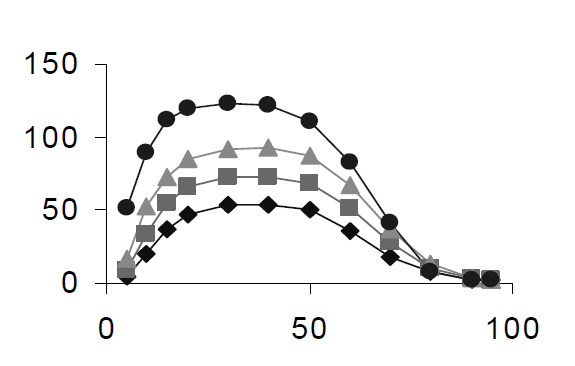
\includegraphics[width=\textwidth]{ch4_figs/hi05_fig7_lifetime}
	\caption{Kite/Dart Lifetime to Stability Graph: x-axis = Initial Percentage of ON states, y-axis = Average Lifetime to Stability}
\end{subfigure}
~
\begin{subfigure}[t]{0.6\textwidth}
	\centering
	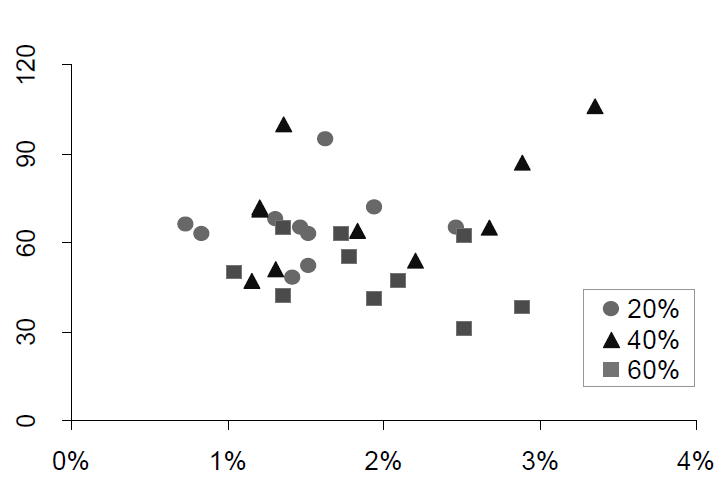
\includegraphics[width=\textwidth]{ch4_figs/hi05_fig8_ash_density}
	\caption{Kite/Dart Ash Density Scatter Plot: x-axis = Ash Density, y-axis = Lifetime to Stability}
\end{subfigure}
\caption[\citeauthor{hi05}'s Kite/Dart Lifetime and Ash Density Graphs]{
	Lifetime to Stability and Ash Density graphs for various sized Kite/Dart tilings produced by \citeauthor{hi05}. In Figure (a), the four graphs correspond Penrose grids of increasing size, with the S grid containing 688 tiles, the M grid containing 1,907 tiles, the L grid containing 5,170 tiles, and the XL grid containing 13,900 tiles. The data points pictured in the scatter plot in Figure (b) are from the M grid~\cite{hi05}.
}
\label{fig:hi05_lifetime_density}
\end{figure}

\begin{figure}[htp]
\centering
\begin{subfigure}[t]{0.6\textwidth}
	\centering
	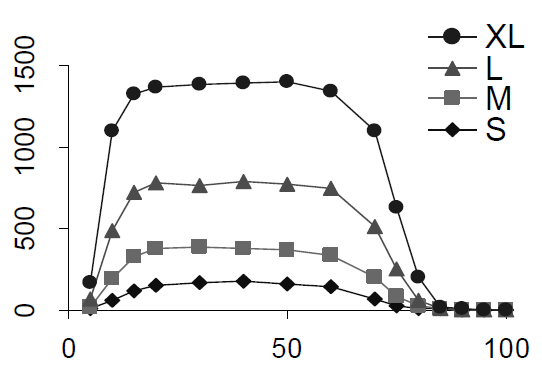
\includegraphics[width=\textwidth]{ch4_figs/hi05_fig6_lifetime}
	\caption{Standard GoL Lifetime to Stability Graph: x-axis = Initial Percentage of ON states, y-axis = Average Lifetime to Stability}
	\label{fig:hi05_reg_lifetime}
\end{subfigure}
~
\begin{subfigure}[t]{0.6\textwidth}
	\centering
	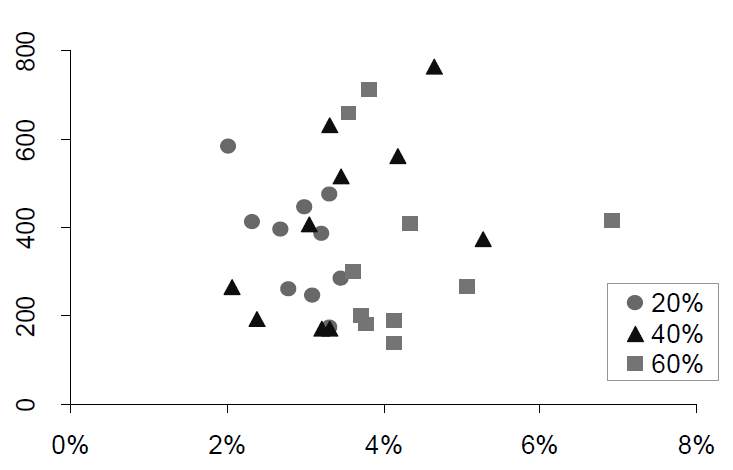
\includegraphics[width=\textwidth]{ch4_figs/hi05_fig8_reg_ash_density}
	\caption{Standard GoL Ash Density Scatter Plot: x-axis = Ash Density, y-axis = Lifetime to Stability}
	\label{fig:hi05_reg_density}
\end{subfigure}

\caption[\citeauthor{hi05}'s Standard GoL Lifetime and Ash Density Graphs]{
	The Lifetime to Stability graph for standard grids produced by \citeauthor{hi05}. The grid sizes were chosen to be as close as possible to their Penrose counterparts, with the S grid containing 676 cells, the M grid containing 1,937 cells, the L grid containing 5,184 cells, and the XL grid containing 13,924 cells. The data points pictured in Figure (b) are from the M grid~\cite{hi05}.
}

\end{figure}

We also collected data for Lifetime to Stability and Ash Density graphs for Rhombs as shown in Figure \ref{fig:crh_lifetime_density}. The lifetime graph for the Rhomb tiling possesses the same overall right-skewed shape as all the other lifetime graphs we have examined, and outside of a few outliers the ash density plot shows no correlation between lifetime and final ash density either. Again, the final ash densities fall within a range of $d=0$ to $d=0.03$ like the Kite/Dart tilings. However, the overall average lifetime for the Rhomb tiling is higher than the lifetimes for the Kite/Dart tiling (Figure \ref{fig:both_lifetime}); we speculate that this is due to the convexity of the Rhomb tiles which allow for larger neighborhood sizes which then allow more opportunities for ON cells to proliferate. We will examine neighborhood differences in more detail in Section \ref{sec:ch4_neighbors}.

\begin{figure}[htp]
\centering
\begin{subfigure}[t]{0.6\textwidth}
	\centering
	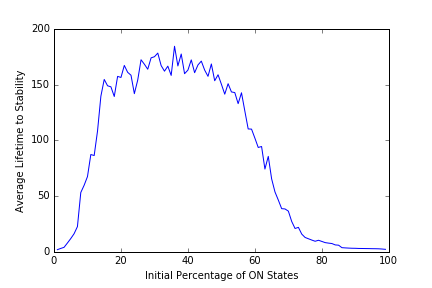
\includegraphics[width=\textwidth]{ch4_figs/crh_lifetime}
	\caption{Rhomb Lifetime to Stability Graph}
\end{subfigure}
~
\begin{subfigure}[t]{0.6\textwidth}
	\centering
	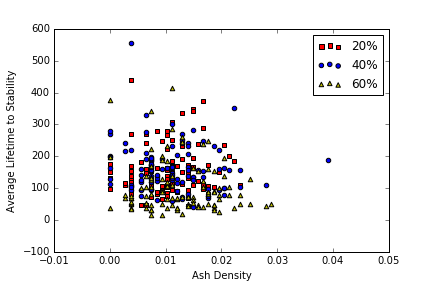
\includegraphics[width=\textwidth]{ch4_figs/crh_ash_density}
	\caption{Rhomb Ash Density Plot}
\end{subfigure}

\caption[Rhomb Lifetime and Ash Density Graphs]{
	Lifetime to Stability and Ash Density graphs for the Rhomb circular tiling, grid size = 1,075. 
}
\label{fig:crh_lifetime_density}
\end{figure}

\begin{figure}[htp]
\centering
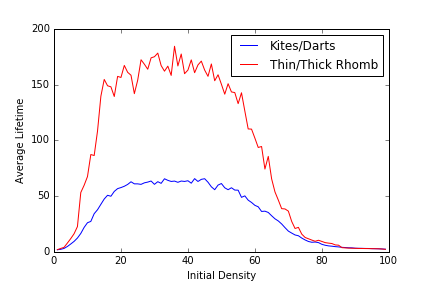
\includegraphics[width=0.6\textwidth]{ch4_figs/both_lifetime}
\caption[Kite/Dart and Rhomb Lifetime Graph]{
	Lifetime graphs for both our circular Kite/Dart and Rhomb tilings. Note the same overall right-skewed distribution for both graphs.
}
\label{fig:both_lifetime}
\end{figure}


\section{Single Run Analysis}
\label{sec:ch4_single_run}
TODO best way to insert sequence of pictures?

%TODO: Circ Kite/Dart longest run: initial percentage=28, seed=92, lifetime=169

The longest run we observed in our Kite/Dart simulations began with an initial soup density of $d=0.22$ and had an active lifetime of 173 timesteps before periodic behavior set in. We graph the active density of ON cells in the tiling against time in Figure \ref{fig:ckd_single}. As seen in this graph, the active density of the Penrose quickly falls to near typical ash density levels ($d \approx 0.03$) and stays close to constant over a majority of its lifetime. We hypothesize that this behavior would be indicative of ash stabilizing relatively quickly with a small glider-like structure being primarily responsible for the long lifetime. Looking at the actual simulation, this seems to be the case, with an amorphous moving structure propagating in the upper left corner for majority of the simulation as seen in Figure TODO. Otherwise, the ash settles relatively quickly, with a \textit{plinker} (coined by \citeauthor{hi05}) period 2 oscillator present on the right side of the tiling.

\begin{figure}[htp]
\centering
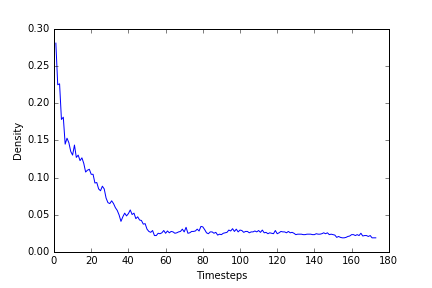
\includegraphics[width=0.6\textwidth]{ch4_figs/ckd_173_density_lifetime}
\caption[Kite/Dart Single Run Density Graph]{
	Active density plotted against time for an initial soup density of $d=0.22$ on our circular Kite/Dart tiling. The lifetime of the run was 173 timesteps, with a final ash density of $d=0.0190$.
}
\label{fig:ckd_single}
\end{figure}

The longest run observed in our Rhomb simulations began with an initial soup density of $d=0.26$ had an active lifetime of 666 timesteps. Its density is plotted against time in Figure \ref{fig:crh_single}. Unlike the Kite/Dart single run, there are some fluctuations in the active density of ON cells in the grid throughout the run. Upon visual inspection of the run (seen in Figure TODO), there is spreading activation across the grid when moving structures collide with stable structures or oscillators, resulting in the spikes in density such as the one beginning around timestep 200.

\begin{figure}[htp]
\centering
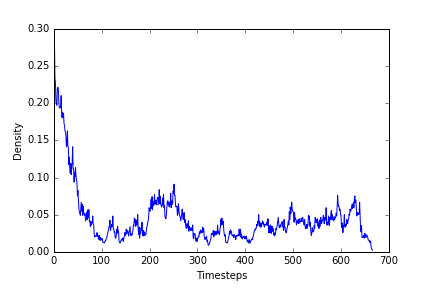
\includegraphics[width=0.6\textwidth]{ch4_figs/crh_666_density_lifetime}
\caption[Rhomb Single Run Density Graph]{
	Active density plotted against time for an initial soup density of $d=0.26$ on our circular Rhomb tiling. The lifetime of the run was 666 timesteps, with a final ash density of $d=0.0279$.
}
\label{fig:crh_single}
\end{figure}

In either run, the most coherent structures are oscillators; ``glider-like'' objects struggle to emerge and move across the grid, with most movement occurring haphazardly across the tilings with no well-defined direction or structural boundaries like standard Game of Life gliders. This was expected due to the aperiodic nature of Penrose tilings, with structural coherency only possible within localized regions of the tiling as neighborhood size and structure will vary across the grid. With the experiments and data collected thus far, it appears that effective information transfer will be difficult to achieve within Penrose Life of either tiling.

\section{Neighborhood Analysis}
\label{sec:ch4_neighbors}

We see a significant difference between the average lifetimes of the Kite/Dart and Rhomb tilings, primarily due to differing local neighborhood characteristics. The possible neighborhood configurations for both tilings are pictured in Figure~\ref{fig:ow08_nbd_stencils}. We see that Rhomb tilings have many stencil configurations with a neighborhood size of ten or greater, while the Kite/Dart tilings only have one such stencil configuration. This is likely to give Rhomb tilings higher average neighborhood sizes across an entire tiling. Neighborhood size frequencies for our circular tilings are pictured in Figure~\ref{fig:both_neighborhood}. The most frequent neighborhood size for our Kite/Dart tiling is 9, whereas the most frequent neighborhood size for our Rhomb tiling is 10. The average neighborhood size is indeed higher for Rhombs than it is for Kite/Darts, as shown in Table~\ref{tbl:avg_nbd}. This data suggests that increased connectivity would allow for longer lifetimes, as there would be more opportunities for birth. Also note that both tilings have a higher neighborhood size than regular square grids, which have a neighborhood size of 8. Thus we cannot solely rely on connectivity when evaluating a grid's ability to support Life or other complex behavior. 

\begin{figure}[htp]
\centering
\begin{subfigure}[t]{0.6\textwidth}
	\centering
	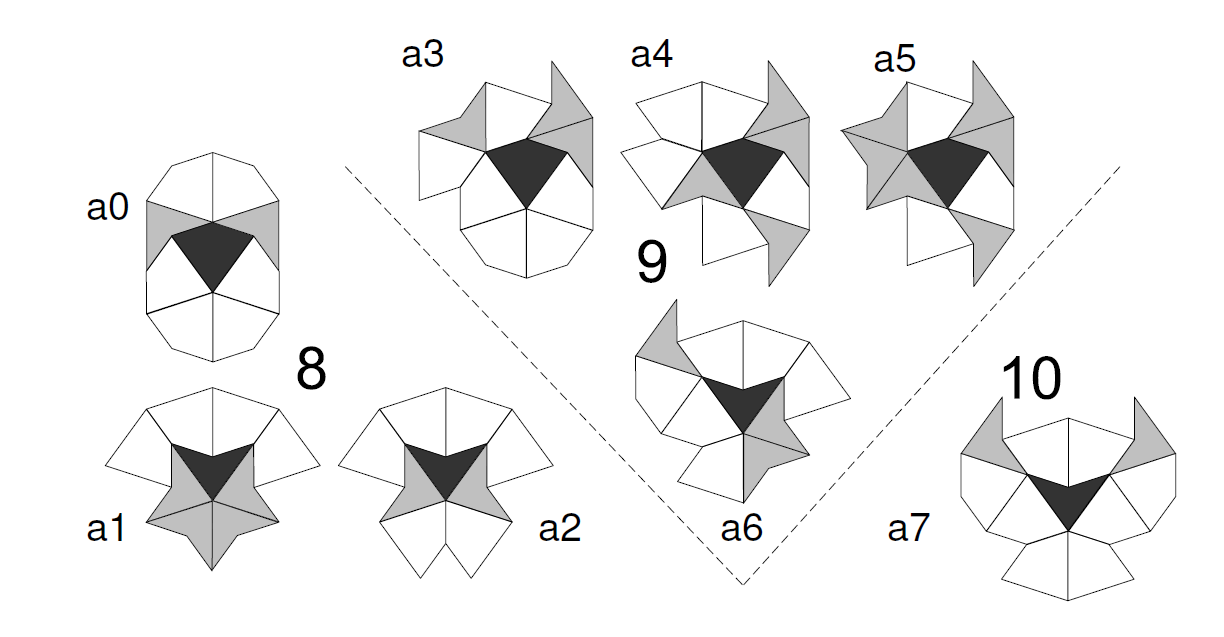
\includegraphics[width=\textwidth]{ch4_figs/ow08_fig18_kd_nbd}
	\caption{Generalized Moore Neighborhood for Kites/Darts}
\end{subfigure}
~
\begin{subfigure}[t]{0.6\textwidth}
	\centering
	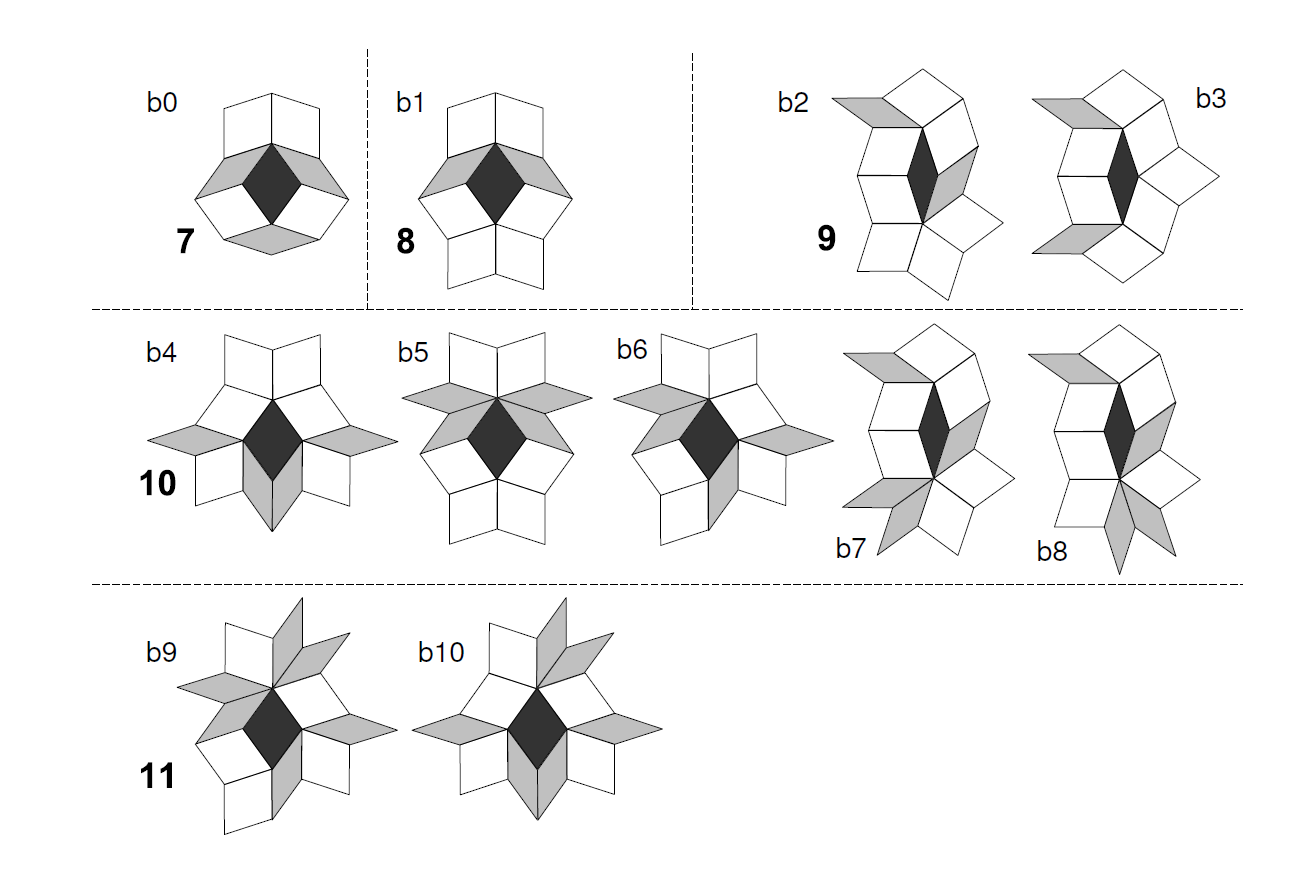
\includegraphics[width=\textwidth]{ch4_figs/ow08_fig20_rh_nbd}
	\caption{Generalized Moore Neighborhood for Rhombs}
\end{subfigure}

\caption[Generalized Moore Neighborhoods for Kites/Darts and Rhombs]{
	All generalized Moore neighborhood stencils for both Kites/Darts and Rhombs. The size of the neighborhood is shown in bold. Figures adapted from 
	\citeauthor{ow08}~\cite{ow08}.
}
\label{fig:ow08_nbd_stencils}
\end{figure}

\begin{figure}[htp]
\centering
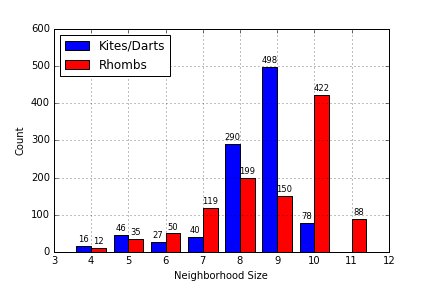
\includegraphics[width=0.6\textwidth]{ch4_figs/both_neighborhood_size}
\caption[Kite/Dart and Rhomb Neighborhood Size Frequency]{
	A histogram of neighborhood size frequency for both our Kite/Dart and Rhomb grid. Note that neighborhood sizes of less than 8 for Kites/Darts and less than 7 for Rhombs belong to border tiles with incomplete neighborhoods.
}
\label{fig:both_neighborhood}
\end{figure}

Because tiles on the boundary have incomplete neighborhoods, we may get differing behavior at the border of the tiling that may impact lifetime or ash density. To investigate potential impact of border tiles, we recorded the neighborhood frequency for the Rhomb single run discussed in Section~\ref{sec:ch4_single_run}, pictured in Figure~\ref{fig:crh_single_nbd}. Neighborhood sizes of 6 or less only occur at the boundaries, making them incomplete neighborhoods for the Rhomb tiling. Since we do see some activity throughout the lifetime of the simulation at these border cells, we need to consider ways to examine boundary effects. One option we explore in the following section is to place an initial starting configuration within a subregion of a larger graph and then only consider activity in the subregion.

\begin{figure}[htp]
\centering
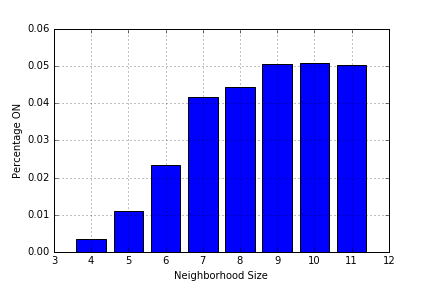
\includegraphics[width=0.6\textwidth]{ch4_figs/crh_666_neighbor_on_percent}
\caption[Rhomb Single Run Neighborhood ON Percentage]{
	A chart of the ON percentage of neighborhood sizes. We record the number of ON cells with a particular neighborhood size and divide by the total number of cells with that neighborhood size for each timestep, averaging across all timesteps.
}
\label{fig:crh_single_nbd}
\end{figure}

\begin{figure}[htp]
\centering
\begin{tabular}{| l | l |}
\hline
Kite/Dart & Rhomb \\
\hline
8.360 & 8.824 \\
\hline
\end{tabular}
\caption[Kite/Dart and Rhomb Average Neighborhood Size]{
1	Kite/Dart and Rhomb Average Neighborhood Size
}
\label{tbl:avg_nbd}
\end{figure}

\section{Subregion Analysis}

As shown by \citeauthor{hi05} in Figure~\ref{fig:hi05_lifetime_density}, the size of the grid impacts the average lifetime. In order to investigate both border and size effects on the lifetime of Penrose Life, we ran \textit{subregion} experiments.

\subsection*{Experimental Setup}
We generated much larger circular Kite/Dart (6484 tiles) and Rhomb (7007 tiles) tilings, but only initialized a subregion of the tiling (Figure~\ref{fig:crhx_sub_init}). The subregion radius is chosen to match the smaller grid we have previously analyzed as close as possible with the idea of replicating the original starting configurations of our first set of lifetime experiments but providing more grid space and removing boundary cell effects. Lifetime to Stability and Ash Density are calculated in the same manner with the same number of trials as before, with 100 different initial configurations for each initial soup density $d=0.01...0.99$ giving 9900 total trials. Ash density is only measured within the subregion.

\begin{figure}[htp]
\centering
\includegraphics[width=0.6\textwidth]{ch4_figs/crhx_subregion}
\caption[Rhomb Subregion Initialization]{
	An illustration of subregion initialization for our large Kite/Dart tiling (6484 tiles). The initial soup density within the subregion is $d=0.09$.
}
\label{fig:crhx_sub_init}
\end{figure}

\subsection*{Results}
The Lifetime to Stability graph comparing our initial Kite/Dart tiling to the larger subregioned tiling is shown in Figure~\ref{fig:ckd_small_large_lifetime}. There is not a significant increase in lifetime at the peak initial soup densities, though the larger grid appears to have less of a fall-off of average lifetime at higher initial densities. The analogous graph for Rhomb tilings is shown in Figure~\ref{fig:crh_small_large_lifetime}. For Rhombs, we do see a large increase in lifetimes across all densities. The differences between Kite/Darts and Rhombs in average lifetimes for large tilings could be due to the relative increased connectivity of the large Rhomb tilings when there are no boundaries present: if we take the weighted average of incomplete neighborhood sizes for both Kite/Darts and Rhombs as shown in Figure~\ref{fig:both_neighborhood}, the Kite/Dart average incomplete neighborhood size (6.27) is higher than the Rhomb incomplete neighborhood size (5.12). Coupled with the fact Rhomb tilings have a larger average neighborhood size (Figure~\ref{tbl:avg_nbd}), the ``removal'' of boundaries from the subregioned tilings would produce a more dramatic change in neighborhood sizes for the Rhomb tiling in comparison to the Kite/Dart tiling. This difference could also potentially be due to other factors, such as the geometric or spatial orientation of the two different types of Penrose tilings.

%6.27
%5.12

\begin{figure}[htp]
\centering
	\begin{subfigure}[t]{0.6\textwidth}
	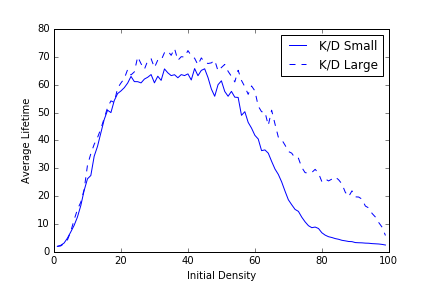
\includegraphics[width=\textwidth]{ch4_figs/ckd_small_large_lifetime}
	\caption{Kite/Dart Small/Large Lifetime Graph}
	\label{fig:ckd_small_large_lifetime}
	\end{subfigure}
~
	\begin{subfigure}[t]{0.6\textwidth}
	\centering
	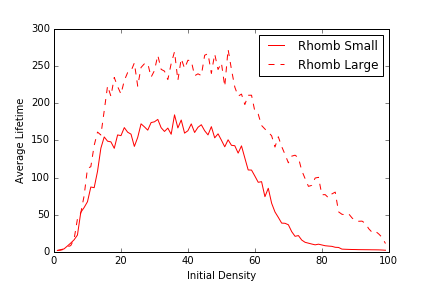
\includegraphics[width=\textwidth]{ch4_figs/crh_small_large_lifetime}
	\caption{Rhomb Small/Large Lifetime Graph}
	\label{fig:crh_small_large_lifetime}
	\end{subfigure}
\caption[Small/Large Lifetime Graphs]{
	Average Lifetime plotted against Initial Density for both our small Penrose tilings and our large subregion Penrose tilings.
	}
\end{figure}

Ash density scatter plots for our subregion Kite/Dart and Rhomb tilings are pictured in Figure~\ref{fig:ckd_sub_ash_density} and Figure~\ref{fig:crh_sub_ash_density}. Note that the ash density values are only measured within the subregion of initialization; ash in the outer regions of the tiling are not included in the density calculation. We see again that there is no correlation between lifetime and ash density as shown by both plots, and the ash densities fall roughly the same ranges we have seen before. In Figure~\ref{fig:crh_sub_ash_density} there are a number of simulations that have a final ash density of zero for Rhomb tilings. This could be due to moving structures that travel outside the subregion, which makes sense as the average lifetime for Rhomb tilings is also much higher than the average lifetime for Kite/Dart tilings. These subregion experiments illustrate that Rhomb tilings may have fundamental properties  different from the Kite/Dart tilings beyond neighborhood size that allow for long-lived Penrose Life runs. 
%Overall however, it appears that ``removing'' the boundary from the Penrose tilings does not significantly alter the quantitative behavior of either type of tiling.

\begin{figure}[htp]
\centering
	\begin{subfigure}[t]{0.6\textwidth}
	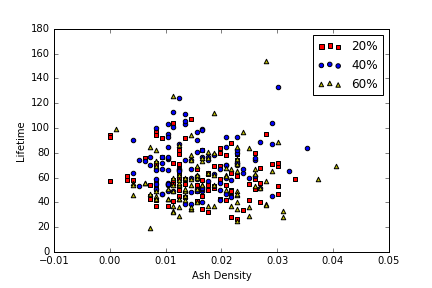
\includegraphics[width=\textwidth]{ch4_figs/ckdx_sub_ash_density}
	\caption{Kite/Dart Subregion Ash Density Scatter Plot}
	\label{fig:ckd_sub_ash_density}
	\end{subfigure}
~
	\begin{subfigure}[t]{0.6\textwidth}
	\centering
	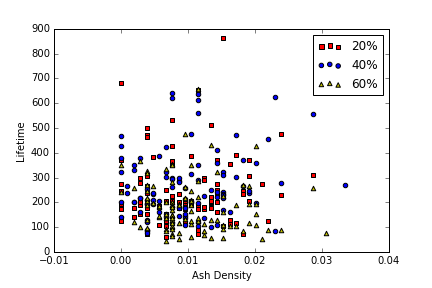
\includegraphics[width=\textwidth]{ch4_figs/crhx_sub_ash_density}
	\caption{Rhomb Subregion Ash Density Scatter Plot}
	\label{fig:crh_sub_ash_density}
	\end{subfigure}
\caption[Subregion Ash Density Plots]{
	Ash Density scatter plots for both Kite/Dart and Rhomb subregion tiling. Ash density is only measured from within the initialization subregion.
	}
\end{figure}

\section{Potential for Penrose Gliders}
With the ash density results shown for subregion Rhomb tilings along with the significantly higher average lifetime for Rhomb tilings in general, there is some potential for gliders to be found in Penrose Rhomb Life. Unfortunately, like \citeauthor{ow10} who also searched for gliders in Penrose tilings~\cite{ow10}, the only coherent structures we have detected in either tiling are oscillators. It appears that the aperiodic nature of the Penrose tilings severely limits the ability for coherent structures to travel beyond a particular localized region within Penrose Life. 

However, if we move away from the Game of Life rules, there is potential for coherent moving structures to exist on Penrose tilings. \citeauthor{go12} created a 4-state CA rule table that supports a coherent glider structure on both Kite/Dart and Rhomb tilings (Figure TODO)~\cite{go12}. This discovery illustrates that aperiodicity does not completely limit the ability for a CA to transfer information across a grid space; in fact it has been conjectured that a CA rule table can be created for \textit{any} quadrilateral tiling, provided that the CA has enough possible states~\cite{mu16}. Further analysis of \citeauthor{go12}'s CA rule table will be conducted in Chapter~\ref{ch:lambda_degen}.

\iffalse
TODO
\begin{itemize}
\item run lambda experiments for K=4, N=11 grids? (Penrose glider)
\end{itemize}
\fi

\section{Summary}
We have conducted various tests examining the behavior of the Game of Life on aperiodic Penrose tilings. By replicating and extending the work of \citeauthor{hi05} to both Kite/Dart and Rhomb tilings, we have shown that though Penrose Life has some similar qualitative properties to the standard Game of Life, there are significant differences in terms of lifetime and ash density between the two CAs. We see that the aperiodicity of the Penrose tilings hampers the ability for information transfer to occur across the grid as the only coherent structures we have detected in our simulations are oscillators. 

Additionally, there appear to be some quantitative differences between the Kite/Dart and Rhomb tiling's ability to support Penrose Life as evidenced by the much higher average lifetimes of simulations on the Rhomb tilings. Possible sources of these differences could be the higher average neighborhood size or the geometric properties (Rhombs are all convex quadrilaterals) of the Rhomb tilings. Boundary conditions and overall grid size also appear to impact a grid's ability to support complex CA behavior. These attributes of irregular grids will be examined further in the following chapters.

\processdelayedfloats

%CHAPTER 5

\chapter{Local Majority Experiments}
\label{ch:local_maj}

As discussed in Chapter~\ref{sec:Robust}, \citeauthor{me07} investigated CA performance on the majority task in the presence of various irregularities. We extend this work by examining the effects of spatial irregularity on CA majority task performance.

\section{Baseline Majority Task Performance on Irregular Grids}

Our extensions of majority task experiments will focus on the \textit{local majority} rule table for 2-state cellular automata. The rules are simple:

\begin{itemize}
\item If there is a majority of ON or OFF cells in a cell $c$'s neighborhood, then $c$ will transition to the majority state.
\item If there is no majority, $c$ will retain its previous state.
\end{itemize}

This rule table represents the most basic manner of solving the majority task and is easily extended to grids with variable neighborhood sizes.

\subsection*{Experimental Setup}
We mirror \citeauthor{me07}'s experimental setup in order to compare our results with theirs. For regular grids, a 15 by 15 grid (225 total cells) is utilized with periodic boundaries. We begin with a 1:99 ON/OFF ratio, incrementing by 1 percent up to 99:1. The simulation is run for a maximum of 450 time steps, recording only completely correct classification. 1,000 random grid configurations are used for every starting ratio, giving a total of 99,000 trials. A single complete run takes approximately 25 minutes in our simulation system.

We use Delaunay and Voronoi generation methods to generate our irregular grids. Our experiments utilize both a grid created through Poisson Disk generator points (Figure~\ref{fig:lm_delaunay}) as well as a grid created through a plant stomatal array. For the stomatal array, we begin with an image of the stomata and drop points where the stoma are located. We then utilize these points as generator points for a Delaunay triangulation. The entire process is pictured in Figure~\ref{fig:stoma_graph_gen}.

\begin{figure}[htp]
\centering
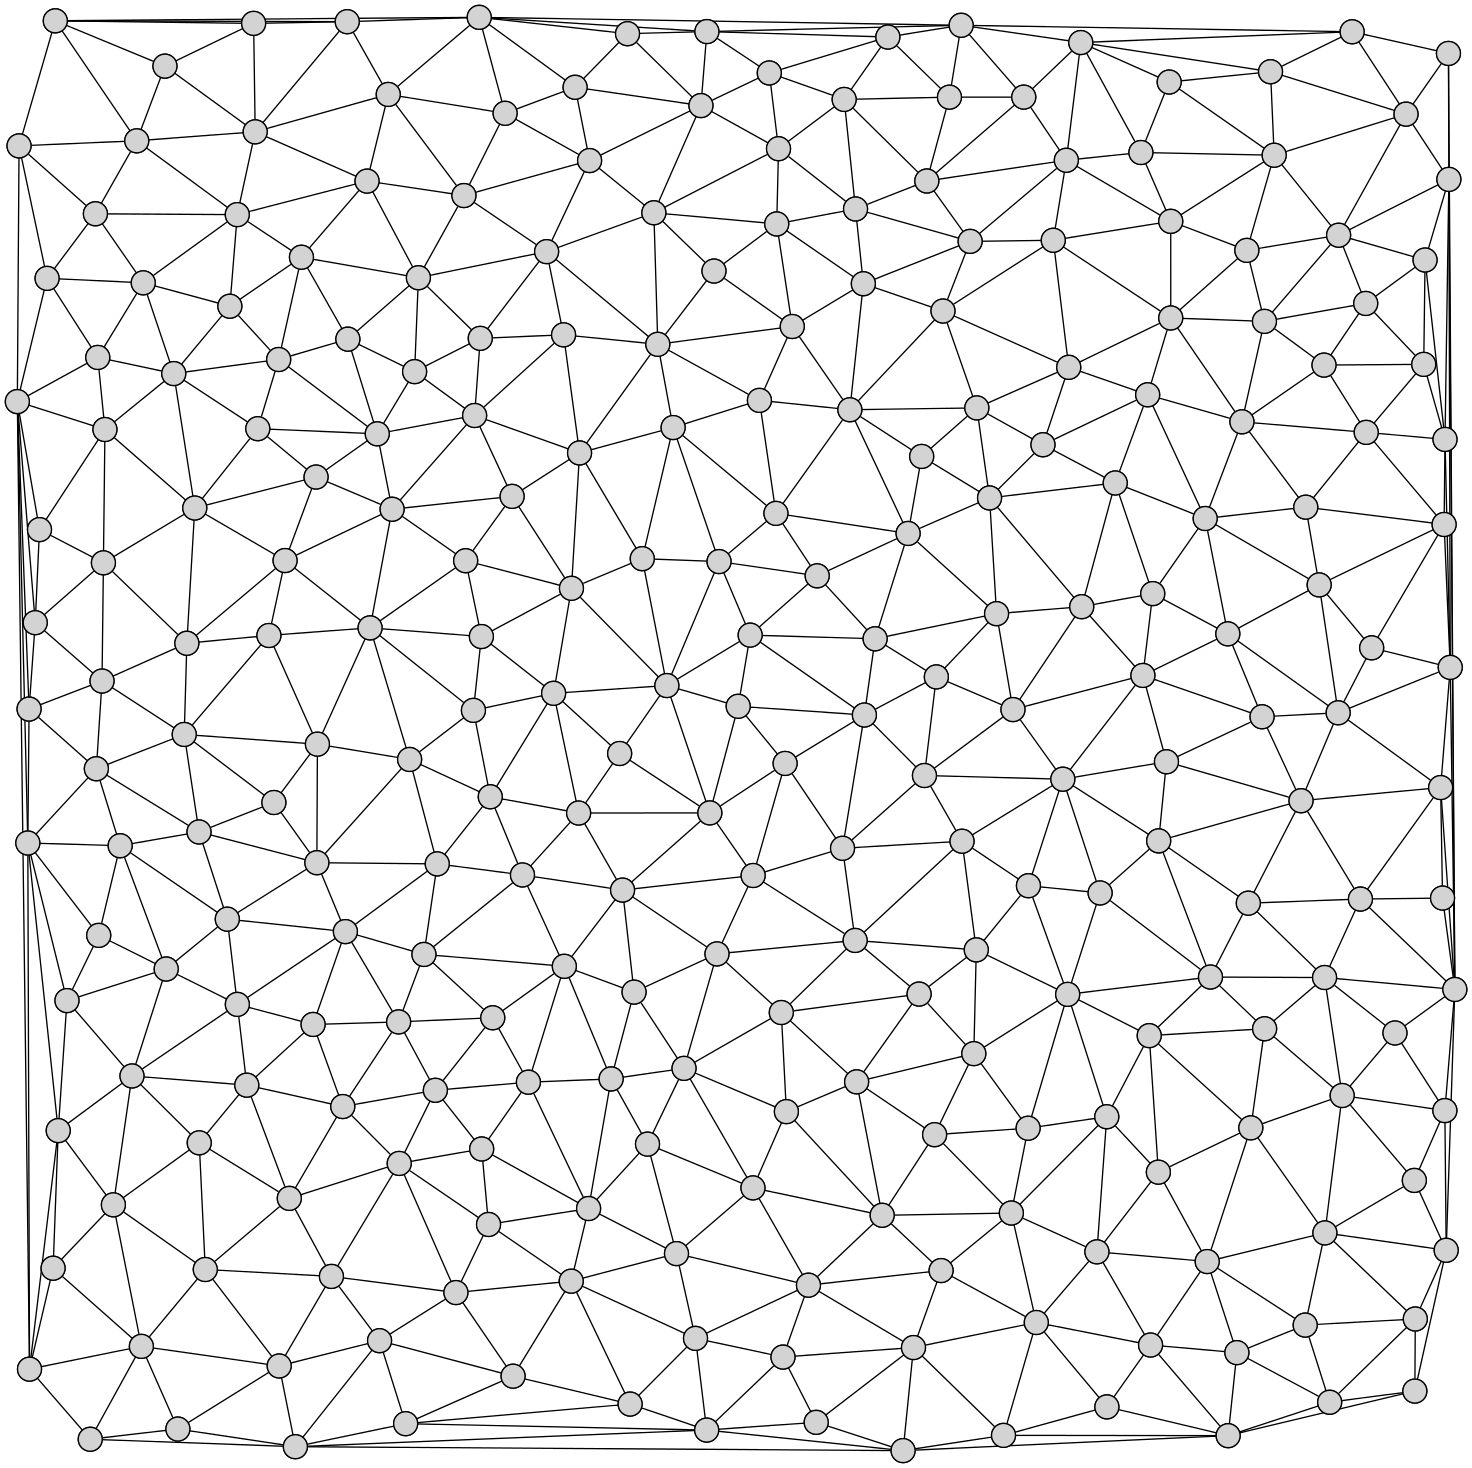
\includegraphics[width=0.6\textwidth]{ch5_figs/lm_delaunay}
\caption[Irregular Delaunay Grid for Majority Task]{
  The Delaunay Triangulation (and thus connectivity graph) for our generated irregular grid. Dimensions for the Poisson Disk sampling were chosen so that the cell count would match the 15 by 15 size of the baseline regular grid as close as possible.
}
\label{fig:lm_delaunay}
\end{figure}


\begin{figure}[htp]
\centering
  \begin{subfigure}[t]{0.55\textwidth}
  \includegraphics[width=\textwidth]{ch5_figs/stoma}
  \caption{Original Stomatal Array Image}
  \end{subfigure}
  ~
  \begin{subfigure}[t]{0.55\textwidth}
  \centering
  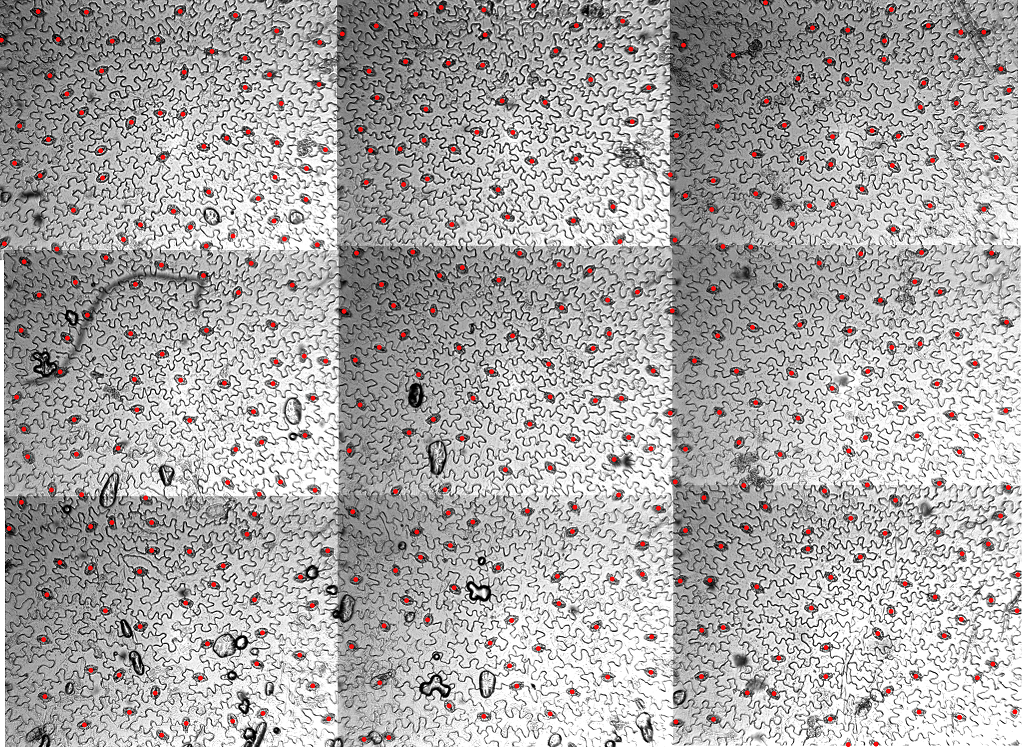
\includegraphics[width=\textwidth]{ch5_figs/stoma-colored}
  \caption{Stomatal Array with Stomata Marked}
  \end{subfigure}
  ~
  \begin{subfigure}[t]{0.55\textwidth}
  \centering
  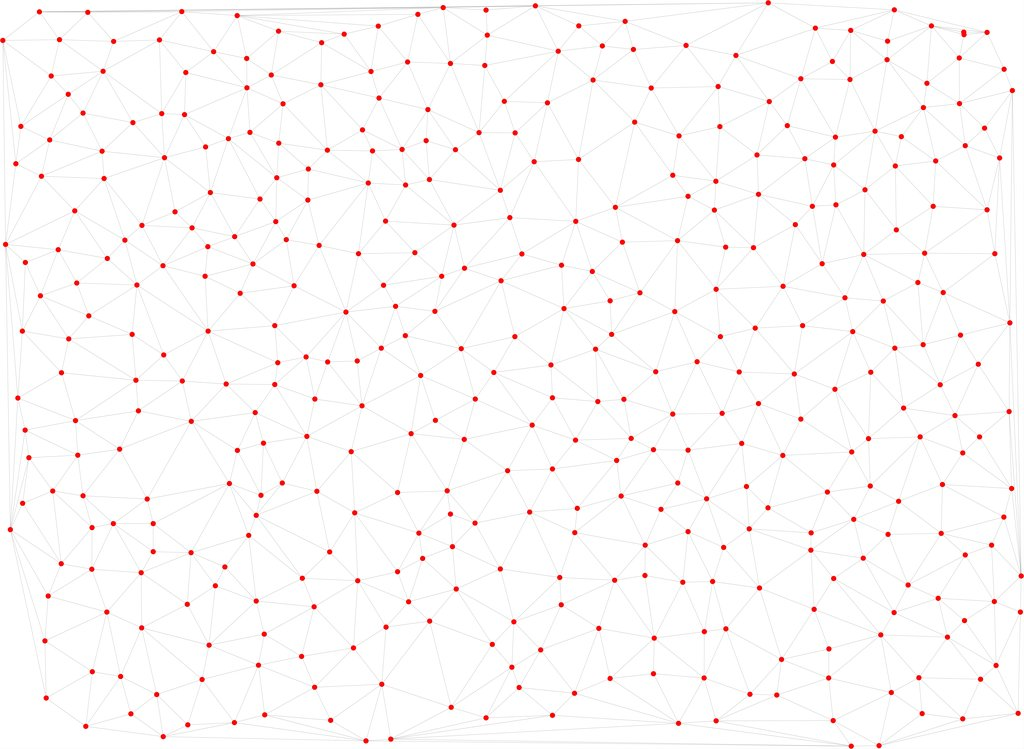
\includegraphics[width=\textwidth]{ch5_figs/stoma_graph}
  \caption{Stomatal Delaunay Triangulation}
  \end{subfigure}
\caption[Grid Generation from Stomatal Array]{
  An illustration of the process we use to generate a grid from a stomatal array image. The final grid pictured is the Delaunay Triangulation of the generator points, which corresponds to the connectivity graph we utilize for the majority task CA.
  }
\label{fig:stoma_graph_gen}
\end{figure}

\subsection*{Results}
First we replicated \citeauthor{me07}'s baseline experiments to confirm the accuracy of our system, with our results corresponding exactly with theirs (Figure~\ref{fig:me07_baseline_rep}). The general profile of the Local Majority Task performance curve is symmetric, with a severe fall-off in task performance at around ON/OFF ratios of 15:85 and 85:15 and 0\% task performance between ratios of about 30:70 to 70:30. Since the majority classification tasks become increasingly difficult as the ON/OFF ratio approaches 50:50, this degradation in performance is to be expected for such a simple rule. For comparison, the task performance of a more complex rule table created through the use of a \textit{genetic algorithm} is also pictured in Figure~\ref{fig:me07_baseline}. The overall performance of this rule table is much better than the local majority rule, but also sees a drop in performance when classifying 50:50 initial ratios.

\begin{figure}[htp]
\centering
  \begin{subfigure}[t]{0.6\textwidth}
  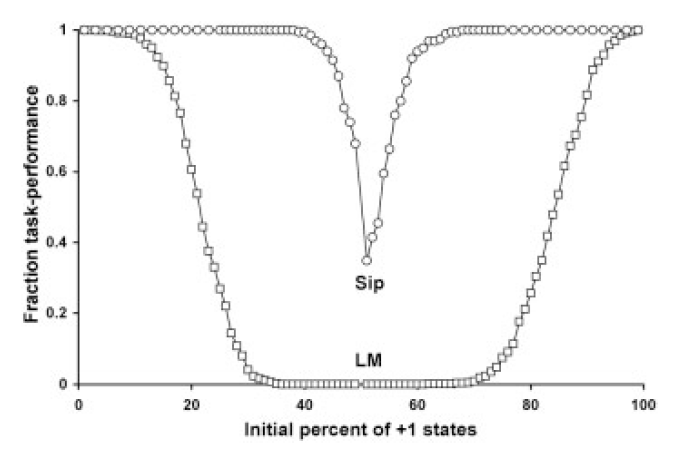
\includegraphics[width=\textwidth]{ch5_figs/me07_fig2_LMBaseline}
  \caption{\citeauthor{me07}'s Baseline Local Majority Task Performance Graph}
  \label{fig:me07_baseline}
  \end{subfigure}
  ~
  \begin{subfigure}[t]{0.6\textwidth}
  \centering
  \includegraphics[width=\textwidth]{ch5_figs/lm_baseline_reg_tor}
  \caption{Replicated Baseline Local Majority Task Performance}
  \end{subfigure}
\caption[Replication of \citeauthor{me07}'s Baseline Local Majority Performance]{
  An illustration of baseline Local Majority task performance on square, periodic 15 by 15 grid. We achieve the same performance graph as \citeauthor{me07}, which is labeled LM in Figure~\ref{fig:me07_baseline}. The performance graph labeled Sip in Figure~\ref{fig:me07_baseline} is from a CA rule table created through the use of a genetic algorithm~\cite{me07}.
}
\label{fig:me07_baseline_rep}
\end{figure}

The task performance of our two irregular grids are pictured in Figure~\ref{fig:lm_ireg}. We see that both irregular grids have the same symmetric task performance profile as the baseline regular grids. This result suggests that irregular grids could be suitable for supporting complex behavior comparable to regular grids. It is also important to note that both irregular grids lack periodic boundary conditions unlike the baseline regular case. The absence of periodicity decreases neighborhood connectivity and will hurt a CA's ability to transfer information across the grid space, making the task performance of the irregular grids even more remarkable. For comparison, local majority task performance for regular grid is reduced significantly when periodic boundary conditions are removed, shown in Figure~\ref{fig:lm_reg_nonper}. Thus, it appears that in the context of the majority task, spatial irregularity will not hinder the performance or behavior of a CA system. The fact that local majority task performance is essentially equivalent across both square and spatially irregular grids establishes a rough form of equivalence between the two grid types within the domain of the CA majority task.

\begin{figure}[htp]
\centering
  \begin{subfigure}[t]{0.6\textwidth}
  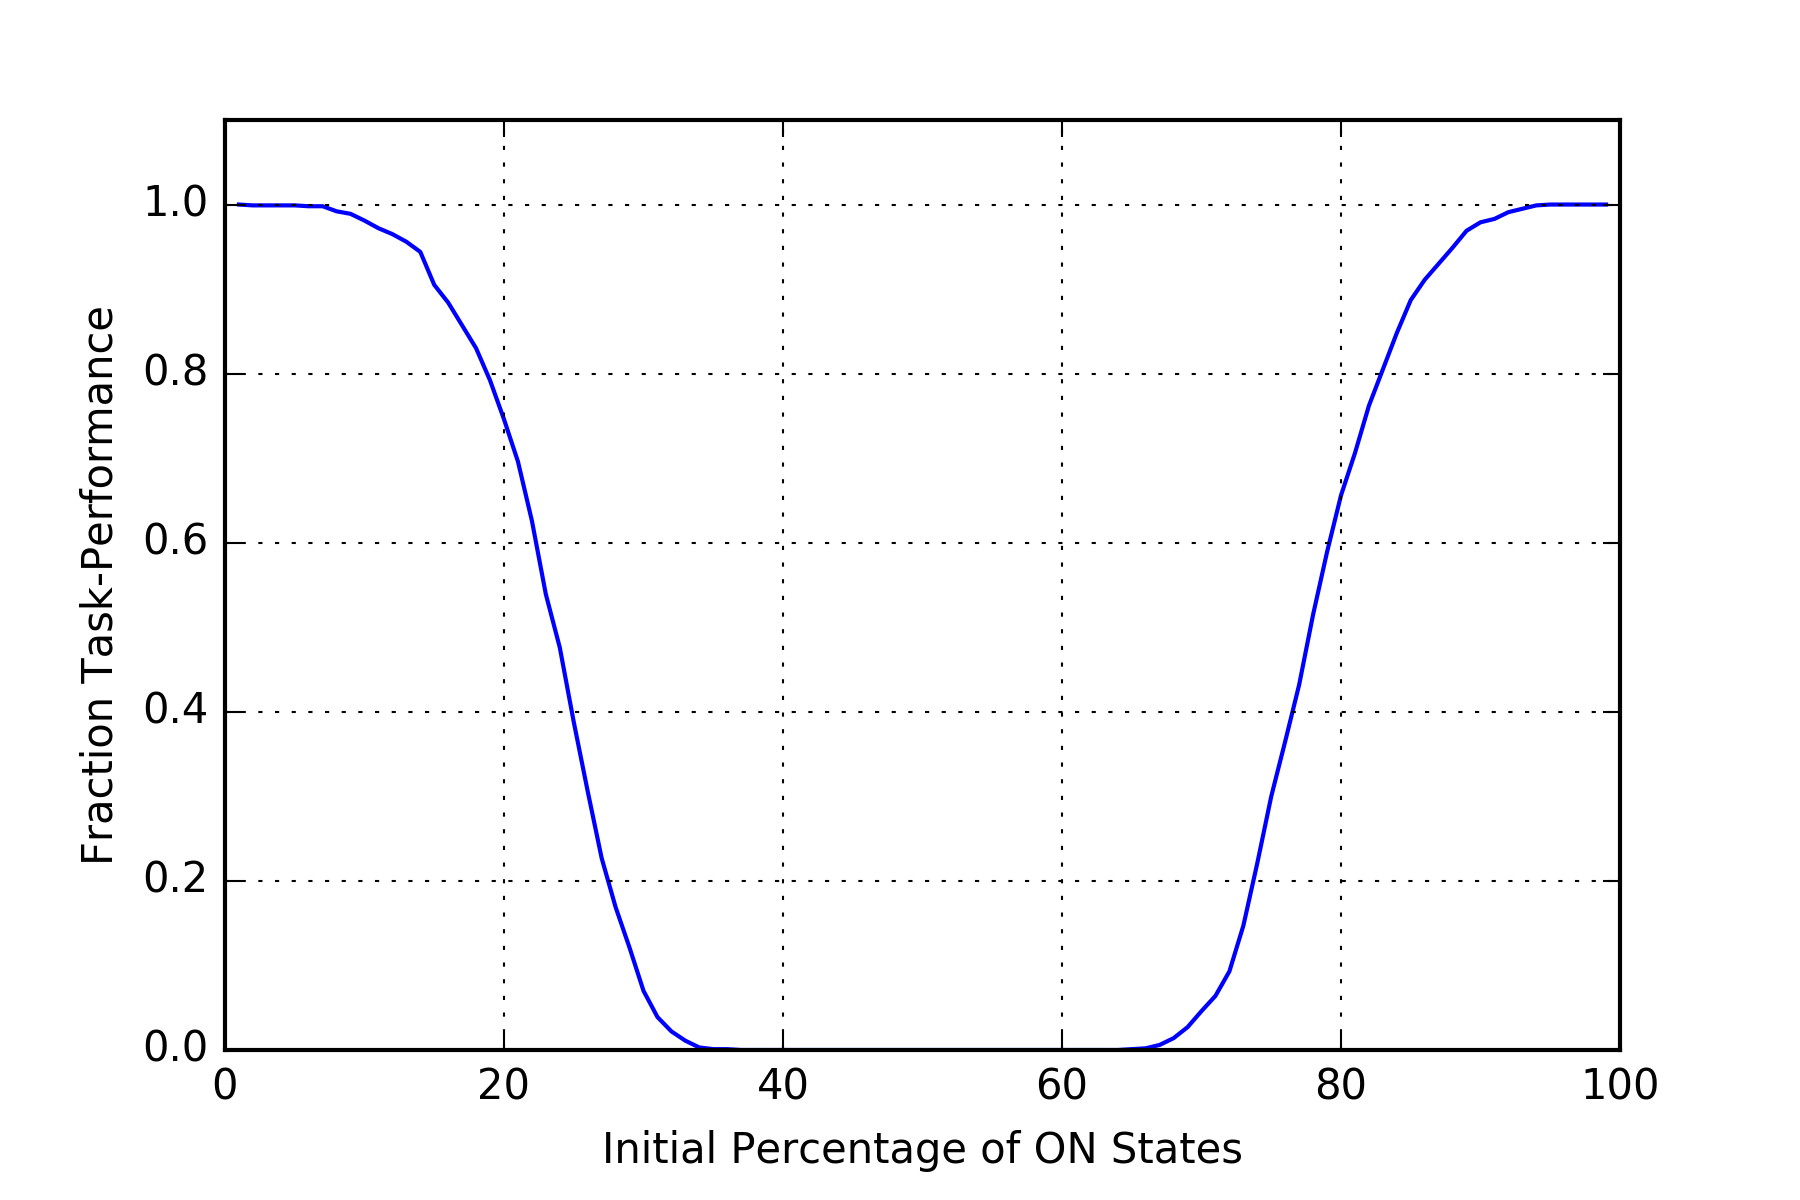
\includegraphics[width=\textwidth]{ch5_figs/LM_baseline_vor}
  \caption{Local Majority Task Performance on a Voronoi Grid}
  \end{subfigure}
  ~
  \begin{subfigure}[t]{0.6\textwidth}
  \centering
  \includegraphics[width=\textwidth]{ch5_figs/lm_baseline_stoma}
  \caption{Local Majority Task Performance on a Stoma Grid}
  \end{subfigure}
\caption[Local Majority Task Performance on Irregular Grids]{
  Task Performance graphs for both our generated irregular grid and the stoma irregular grid. Both have almost identical performance profiles to the baseline Local Majority task performance graph for regular grids.
}
\label{fig:lm_ireg}
\end{figure}

\begin{figure}[htp]
\centering
\includegraphics[width=0.6\textwidth]{ch5_figs/lm_baseline_reg_nontor}
\caption[Local Majority Task Performance on a Non-Periodic Regular Grid]{
  The task performance graph for a 15 by 15 regular grid with non-periodic boundary conditions. Notice the degradation in task performance in comparison to the performance graphs in Figure~\ref{fig:me07_baseline_rep}.
}
\label{fig:lm_reg_nonper}
\end{figure}

\section{Majority Task Performance with State Noise}

\citeauthor{me07} discovered in their investigations that introducing small amounts of state noise improves the performance of majority task CA, likely due to the fact that the random state change will stimulate movement across the grid~\cite{me07}. We will investigate the impact of state noise in more detail and in the context of irregular grids. 

\subsection*{Experimental Setup}

Data for task performance graphs is collected with the same setup and number of trials as in the previous section. State noise is introduced by changing each cell's correct output state with probability $\eta$ before the next timestep. State noise is not applied if the CA has reached a uniform configuration of either all ON or all OFF states. Since \citeauthor{me07} reported that state noise probabilities of $\eta \ge 0.1$ caused massive degradation of majority task performance, we consider a range of state noise from $\eta=0.01$ to $\eta=0.15$.

Since initial ON/OFF ratios near 50:50 are the most difficult starting configurations to classify, we also perform experiments that measure the impact of state noise on ``hard'' initial configurations. For each state noise percentage, we generate 1,000 random initial configurations with ON/OFF ratios chosen from a Gaussian distribution $\mathcal{N}(0.5, 0.06)$.

\subsection*{Results}

Task performance graphs for regular grids with state noise $\eta=0.05$ and $\eta=0.15$ are shown in Figure~\ref{fig:lm_reg_noise}. We see that with an introduction of a small amount of noise ($\eta=0.05$) task performance dramatically improves, with incorrect classifications only occurring between ON/OFF ratios of 40:60 and 60:40 and with roughly 35\% correct classifications of 50:50 starting ratios. Conversely, when too much noise is introduced to the system ($\eta=0.15$), task performance across all starting ratios degrade below baseline levels. The task performance graphs for the irregular stoma grid with $\eta=0.05, 0.15$ also exhibit the same trend (Figure~\ref{fig:lm_stoma_noise}). However, for the stoma grid with $\eta=0.05$ only about 10\% of the 50:50 starting ratios are correctly classified, which is much poorer performance on 50:50 configurations compared to the regular grid. Overall however, the regular and irregular grids exhibit the same sort of behavior when varying levels of state noise are applied. With the addition of small amounts of state noise, the basic Local Majority rule table performs similarly to more complex rule tables; the performance graph for both regular and irregular grids at $\eta=0.05$ closely resembles the performance graph of the Sip rule pictured in Figure~\ref{fig:me07_baseline}, one of the best performing rule tables evaluated by \citeauthor{me07}~\cite{me07}.

\begin{figure}[htp]
\centering
  \begin{subfigure}[t]{0.6\textwidth}
  \includegraphics[width=\textwidth]{ch5_figs/baseline_noise_5}
  \caption{Local Majority Task Performance on a Regular Grid with 5\% Noise}
  \end{subfigure}
  ~
  \begin{subfigure}[t]{0.6\textwidth}
  \centering
  \includegraphics[width=\textwidth]{ch5_figs/baseline_noise_15}
  \caption{Local Majority Task Performance on a Regular Grid with 15\% Noise}
  \end{subfigure}
\caption[Local Majority Task Performance for Regular Grids with Noise]{
  Majority Task Performance graphs for regular grids with state noise $\eta = 0.05, 0.15$. Note the relative increase and decrease in task performance for low and high amounts of noise, respectively.
}
\label{fig:lm_reg_noise}
\end{figure}

\begin{figure}[htp]
\centering
  \begin{subfigure}[t]{0.6\textwidth}
  \includegraphics[width=\textwidth]{ch5_figs/stoma_noise_5}
  \caption{Local Majority Task Performance on the Stoma Grid with 5\% Noise}
  \end{subfigure}
  ~
  \begin{subfigure}[t]{0.6\textwidth}
  \centering
  \includegraphics[width=\textwidth]{ch5_figs/stoma_noise_15}
  \caption{Local Majority Task Performance on the Stoma Grid with 15\% Noise}
  \end{subfigure}
\caption[Local Majority Task Performance for the Stoma Grid with Noise]{
    Majority Task Performance graphs for the irregular stomata grid with state noise $\eta = 0.05, 0.15$. Note that though the shape of the two graphs resemble those in Figure~\ref{fig:lm_reg_noise}, the irregular $\eta=0.05$ graph has a sharper drop-off in 50:50 initial ratio task performance.
}
\label{fig:lm_stoma_noise}
\end{figure}

The results for local majority task performance on ``hard'' configurations on both regular and stoma grids are shown in Figure~\ref{fig:lm_ff}. We see that task performance significantly increases when state noise $\eta \ge 0.02$ and then quickly degrades when state noise $\eta \ge 0.12$ for both grids. In the regular case, task performance stays relatively steady just above 70\% when $0.02 \le \eta \le 0.12$ while in the irregular stomatal case task performance gradually rises to about 60\% correct classification in that same state noise range. These results confirm that small amounts of state noise is beneficial for majority task performance, regardless of the spatial dynamics of the grid. These results also confirm the viability of irregular Voronoi grids in supporting majority task behavior, with task performance on the stomatal grid closely resembling the results on regular grids throughout all these experiments.

\begin{figure}
\centering
  \begin{subfigure}[t]{0.6\textwidth}
  \includegraphics[width=\textwidth]{ch5_figs/ff_reg}
  \caption{Regular Grid Task Performance on Hard Configurations}
  \end{subfigure}
  ~
  \begin{subfigure}[t]{0.6\textwidth}
  \centering
  \includegraphics[width=\textwidth]{ch5_figs/ff_stoma}
  \caption{Stoma Grid Task Performance on Hard Configurations}
  \end{subfigure}
\caption[Local Majority Task Performance on ``Hard'' Configurations]{
  Local Majority task performance graphs on ``hard'' configurations for both regular grids and stoma grids. For both grids, task performance improves significantly between $\eta=0.02$ and $\eta=0.12$ before falling at $\eta \ge 0.12$. 
}
\label{fig:lm_ff}
\end{figure}

\section{Summary}

%TODO table of overall classification percentage?

We have evaluated local majority task performance on both regular grids and irregular Voronoi grids. The profiles of the performance graphs show remarkable similarities between the regular and irregular grids in majority task performance. These similarities continue when we examine the impact of state noise, though the irregular grids perform slightly worse than the regular grids when noise is introduced. Still, we see that small amounts of state noise \textit{improve} task performance in both the regular and irregular grid cases, with their overall classification percentages rivaling those of more complex, human-engineered majority task rule tables.

Thus, we see more evidence that randomness can facilitate the function of decentralized dynamic systems, and it seems plausible that biological systems utilizing local communication can overcome spatial irregularity and perform comparably to ``perfect'' CA systems even in noisy environments. Again, we see some evidence that spatially irregular grids can be functionally equivalent to their regular counterparts within a specific CA task domain.

\processdelayedfloats

% CHAPTER 6

\chapter{Lambda Degradation Experiments}
\label{ch:lambda_degen}
The $\lambda$ parameter as established by \citeauthor{la90} is an effective way to parameterize and traverse the CA rule space. And though $\lambda$ may be too ``coarse'' of a parameter to pinpoint precisely where the \textit{critical transition point} is for particular class of CAs (see Chapter~\ref{subsec:edge_chaos}), it is sufficient for detecting whether or not transition events can occur for a given CA. Thus, we apply similar $\lambda$ analysis techniques used by \citeauthor{wo90} to irregular and degraded grids.

\section{The Langton-Wootters $\lambda$ Profile}
Our experiments build off work by \citeauthor{wo90} that specifically examine $K=8, N=5$ CAs. As discussed in Chapter~\ref{subsec:metrics}, \textit{Shannon entropy} is often used to measure the complexity of CA systems. Entropy is plotted against $\lambda$ in \citeauthor{wo90}'s experiments to produce what we call the \textit{Langton-Wootters Profile}, pictured in various forms from different table generation methods in Figure~\ref{fig:lw_profile}.

\subsection*{Generating the Langton-Wootters Profile}

The \textit{table walk-through} method for generating transition tables begins with a $\Delta$ transition function that has $\lambda = 0$. Recalling the definition of $\lambda$ (Appendix~\ref{appA:lambda}), $\lambda=0$ indicates that every rule in $\Delta$ maps to the quiescent state $s_q$. The $\Delta$ table is then \textit{incremented} to a higher $\lambda$ value by randomly replacing some of the transitions to $s_q$ with transitions to the other possible states, uniformly chosen~\cite{la90}. This table generation method has the effect of modifying the ``same'' table, allowing us to track CA behavior for individual runs of CA simulation. The Langton-Wootters Profile generated from the table walk-through method is shown in Figure~\ref{fig:lw_profile_walk}.

The \textit{random table} method for generating transition tables utilizes $\lambda$ as a sampling probability. A $\Delta$ table entry is mapped to the quiescent state with probability $1 - \lambda$, while a non-quiescent state is chosen uniformly from the other possible states with probability $\lambda$~\cite{la90}. The Langton-Wootters Profile generated from the random table method is pictured in Figure~\ref{fig:lw_profile_rand}. Also note that all $\Delta$ transition tables possess \textit{planar isotropy} and \textit{strong quiescence} as detailed in Chapter~\ref{subsec:ch3_lamb}.

Entropy is calculated using the equations shown in Appendix~\ref{appA:entrop}. However, entropy calculations are made only for the asymptotic behavior of a given CA simulation: each CA simulation is run for 1,000 time steps, with entropy only measured after time step 500. So if a particular CA run has a lifetime of less than 500, its entropy value will be 0. This manner of calculating asymptotic entropy leads to numerous entropy measurements of 0, as pictured in both versions of the Langton-Wootters Profile. Also note that for $K=8, N=5$ CA, the maximum entropy is 3 with this maximum value occurring with a $\lambda$ value of 0.875 (Appendix~\ref{appB:max_H}). Thus, all experiments with $K=8, N=5$ CA consider a range of $\lambda$ values from $\lambda = 0.0$ to $\lambda = 0.88$. 

\begin{figure}[htp]
\centering
  \begin{subfigure}[t]{0.6\textwidth}
  \includegraphics[width=\textwidth]{ch6_figs/la90_fig8_lambda_runs}
  \caption{Walk-Through Langton-Wootters Profile}
  \label{fig:lw_profile_walk}
  \end{subfigure}
  ~
  \begin{subfigure}[t]{0.6\textwidth}
  \centering
  \includegraphics[width=\textwidth]{ch6_figs/wo90_fig3_entropy_lambda}
  \caption{Random Table and Theoretical Langton-Wootters Profile}
  \label{fig:lw_profile_rand}
  \end{subfigure}
\caption[The Langton-Wootters Profile]{
  Different forms of the Langton-Wootters Profile. Figure~\ref{fig:lw_profile_walk} shows 50 individual runs of the table-walk-through method of varying $\lambda$. Figure~\ref{fig:lw_profile_rand} shows both a scatter plot of data points collected through the random-table method of varying $\lambda$ and the theoretical Langton-Wootters Profile as predicted by mean-field theory (Appendix~\ref{appA:MFT}). Note how both plots produce the same envelope of data points. Plots adapted from both \citeauthor{la90} and \citeauthor{wo90}~\cite{la90,wo90}.
}
\label{fig:lw_profile}
\end{figure}

\subsection*{Analysis of the Langton-Wootters Profile}

Both renditions of the LW-Profile indicate a bimodal distribution of entropy values, with most data points either collected around $H=0$ or $H \gtrsim 0.85$. There is a region where relatively few data points are observed over $0 \le \lambda \le 0.6$ and $0 < H \le 0.85$. This \textit{transition gap} and bimodal distribution are indicators of a critical transition, illustrating the boundary between non-complex CA with low $H$ values and complex CA with much higher $H$ values. This phenomenon is easy to see in Figure~\ref{fig:lw_profile_walk}, with individual transition table runs showing a sharp increase in entropy from below the gap to above the gap at a certain $\lambda$ value. This gap and sudden jump in $H$ are indications that critical transitions can occur in this particular class of CAs on regular grids. Thus, we will utilize these features of the LW-Profile to evaluate irregular grids on their ability to support complex behavior. 
Also observe that entropy values converge rapidly when $\lambda > 0.6$, an indication of the shift of rule tables from complex (Class IV) to chaotic (Class III) (Chapter~\ref{subsec:metrics}). The most interesting action occurs when the variance of entropy values is high, again corresponding to the critical transition gap and jump in entropy from around $H=0.0$ to $H > 0.85$. \citeauthor{la90} discusses the ``ceiling'' of this transition region, noting that $H \approx 0.84$ is the average entropy value of a commonly occurring low $\lambda$ chaotic rule~\cite{la90}, another indication that the gap in data points for $0 < H \le 0.85$ is indicative of a critical transition.

\section{$\lambda$ Profile of Irregular Grids}

\subsection*{Experimental Setup}

We utilize the table walk-through method when varying $\lambda$ for our experiments, as both line and scatter plots can be generated from the resulting data. Though \citeauthor{wo90} run their CA simulations to 1,000 time steps, we saw no difference in the shape of the LW-Profiles between trials with a maximum time step of 500 and trials with a maximum time step of 1,000 (Figure~\ref{fig:lw_reg_short_long}), so in the interest of efficiency we run our experiments with a maximum of 500 time steps with an asymptotic threshold of 250 time steps. 100 individual table walk-through runs for $K=8, N=5$ CA are made, incrementing $\lambda$ from $0.0$ to $0.88$. Since we are examining the $K=8, N=5$ CA class, we require the cells in our grid to have four neighbors. Thus, grids generated with the Voronoi Quadrilateral technique as discussed in Chapter~\ref{subsec:vquad} are appropriate irregular spaces for considering these CA. We apply the VQuad grid generation technique to a Voronoi diagram generated by a Poisson Disk distribution of generator points and to the Voronoi diagram produced by the stomatal array (Figure~\ref{fig:vquad_stoma_gen}). Additionally, we also examine Penrose grids utilizing the generalized von Neumman neighborhood stencil, which also produces neighborhoods of $N=5$. Both Kite/Dart and Thin/Thick Rhomb grids are considered, shown in Figure~\ref{fig:penrose_circ}.

With irregular grids, periodic boundary conditions are not possible, so boundary cell neighborhoods are ``completed'' by inserting quiescent states. Note that this decision could potentially skew the resultant entropy measurements lower, but we have seen some functional equivalence between periodic and non-periodic grids previously with our experiments in Chapter~\ref{ch:local_maj}. Neighborhood cells are ordered clockwise from the origin; since the $\lambda$ rule tables produced are isotropic only the relative ordering of neighborhood cells matter. Cell state frequencies are measured at every time step, so entropy values are computed as an average over the data points collected after the asymptotic threshold.

\begin{figure}[htp]
\centering
  \begin{subfigure}[t]{0.6\textwidth}
  \includegraphics[width=\textwidth]{ch6_figs/v_stoma_edited}
  \caption{Voronoi Diagram of Stomatal Array}
  \end{subfigure}
  ~
  \begin{subfigure}[t]{0.6\textwidth}
  \centering
  \includegraphics[width=\textwidth]{ch6_figs/q_stoma}
  \caption{VQuad Diagram of Stomatal Array}
  \end{subfigure}
\caption[VQuad Generation from Stomatal Array]{
An illustration of the Voronoi representation of the stomatal array from Figure~\ref{fig:stoma_graph_gen} and the resultant Voronoi Quad grid. 
}
\label{fig:vquad_stoma_gen}
\end{figure}

\begin{figure}[htp]
\centering
  \begin{subfigure}[t]{0.6\textwidth}
  \includegraphics[width=\textwidth]{ch6_figs/reg_entropy_500_scatter}
  \caption{Short Simulation ($t_{max} = 500$) Langton-Wootters Profile}
  \label{fig:lw_profile_short}
  \end{subfigure}
  ~
  \begin{subfigure}[t]{0.6\textwidth}
  \centering
  \includegraphics[width=\textwidth]{ch6_figs/reg_entropy_1000_scatter}
  \caption{Long Simulation ($t_{max} = 1000$) Langton-Wootters Profile}
  \label{fig:lw_profile_long}
  \end{subfigure}
\caption[Langton-Wootters Profile for Short and Long Simulations]{
  Langton-Wootters Profiles for both short and long simulations. The overall shape and distribution of data points throughout the graph are largely identical. Thus, it appears that equivalent asymptotic behavior can be achieved within different time scales. Note that in our scatter plots, darker dots indicate higher frequency of values. So, we can see both the tight convergence of entropy at high $\lambda$ values and the high frequency of runs that do not reach the asymptotic threshold, resulting in an entropy value of 0.
}
\label{fig:lw_reg_short_long}
\end{figure}

\subsection*{Results}

The LW-Profiles for our Poisson Disk and Stomatal Voronoi Quad grids are pictured in Figure~\ref{fig:vor_lw_profile} and Figure~\ref{fig:stoma_lw_profile} respectively. In both cases, despite the irregularity in the cell orientation and the non-periodic boundary conditions, we see a remarkably similar shape in the LW-Profile for the Voronoi Quad grids. Examination of Figures \ref{fig:vor_lw_run} and \ref{fig:stoma_lw_run} show all of the individual CA runs experiencing a significant jump in entropy values at some point, evidence of a transition event. The corresponding scatter plots (Figures \ref{fig:vor_lw_scatter} and \ref{fig:stoma_lw_scatter}) of these graphs show that the transition gap in $0 \le H \le 0.84$ is also sparsely populated. There appear to be slightly more data points found in the gap for the stoma grid scatter plot compared to the Poisson Disk grid plot; we speculate that the size of the grid may have an influence on a CA's ability to compute, and the Poisson Disk grid is significantly larger than the stomatal grid. 

LW-Profiles for the Penrose tilings are pictured in Figure~\ref{fig:penrose_lw_profile}. Though the overall shape of the curves are still in line with the baseline profile, we see some small deviations in the LW-Profile for Rhomb tilings, shown in Figure~\ref{fig:crh_lw_profile}. First, we see that the transition gap contains a fair amount of data points, spanning a much larger range of $\lambda$ than any of the other grids we have examined with points in the gap found at $\lambda < 0.2$. There is also more variance in the data points above the transition gap, producing a slightly looser convergence of entropy as $\lambda$ increases. These discrepancies are surprising given our Penrose Life experiments in Chapter~\ref{ch:penrose} showing that the Rhomb tilings supported longer living structures, which suggests that the grids would be better suited for supporting complex behavior. Thus, there is a need for a way to quantify how these graphs may differ from one another, as visual inspection is not an adequate measure of such differences. Overall however, we see entropy profile behavior equivalent to those seen in the baseline experiments as we vary $\lambda$ across all of these irregular grids, suggesting a functional equivalence between irregular, non-periodic quadrilateral grids and their regular, periodic square counterparts. With the preservation of both the overall shape and a well-defined transition gap of the LW-Profiles we have examined, it appears that complex behavior can be supported in all of these irregular quadrilateral grids.

\begin{figure}[htp]
\centering
\begin{subfigure}[t]{0.6\textwidth}
  \includegraphics[width=\textwidth]{ch6_figs/vor_entropy}
  \caption{VQuad Langton-Wootters Profile (Individual Runs)}
  \label{fig:vor_lw_run}
\end{subfigure}
~
\begin{subfigure}[t]{0.6\textwidth}
  \centering
  \includegraphics[width=\textwidth]{ch6_figs/vor_entropy_scatter}
  \caption{VQuad Langton-Wootters Profile (Scatter Plot)}
  \label{fig:vor_lw_scatter}
\end{subfigure}
\caption[Voronoi Quad Langton-Wootters Profile]{
  The Langton-Wootters Profile for a Voronoi Quad grid generated with a Poisson Disk distribution of 4,032 generator points resulting in a VQuad grid with 11,480 cells. Note how closely the scatter plot for the Voronoi Quad grid resembles the shape of the baseline Langton-Wootters Profile in Figure~\ref{fig:lw_profile}. There are very little points observed within the transition gap, and ceiling of the gap is sharply demarcated. It appears that despite the non-periodic boundary conditions and the irregular spatial distribution of grids, this Voronoi Quad grid is capable of supporting complex CA behavior.
}
\label{fig:vor_lw_profile}
\end{figure}

\begin{figure}[htp]
\centering
\begin{subfigure}[t]{0.6\textwidth}
  \includegraphics[width=\textwidth]{ch6_figs/stoma_entropy}
  \caption{Stoma Langton-Wootters Profile (Individual Runs)}
  \label{fig:stoma_lw_run}
\end{subfigure}
~
\begin{subfigure}[t]{0.6\textwidth}
  \centering
  \includegraphics[width=\textwidth]{ch6_figs/stoma_entropy_scatter}
  \caption{Stoma Langton-Wootters Profile (Scatter Plot)}
  \label{fig:stoma_lw_scatter}
  \end{subfigure}
\caption[Stoma Langton-Wootters Profile]{
  The Langton-Wootters Profile for the Voronoi Quad grid generated from the plant stomatal array (Figure~\ref{fig:vquad_stoma_gen}) resulting in 984 total cells. Like the Poisson Disk VQuad grid, we see a strong resemblance between the overall shape of the graph with the baseline LW-Profile with Figure~\ref{fig:stoma_lw_run} showing the large transition jumps in entropy seen in Figure~\ref{fig:lw_profile}. We do see more ``noise'' within the transition gap region compared to Figure~\ref{fig:vor_lw_scatter}. The size of the grid may be a factor in supporting complex behavior, as the stomatal grid is significantly smaller than the Poisson Disk grid. Still, the equivalence in shape of this plot to the baseline suggests that this stomatal grid can also support complex, class IV CAs.
}
\label{fig:stoma_lw_profile}
\end{figure}

\begin{figure}[htp]
\centering
\begin{subfigure}[t]{0.6\textwidth}
  \includegraphics[width=\textwidth]{ch6_figs/ckd_entropy_scatter}
  \caption{Kite/Dart Langton-Wootters Profile}
  \label{fig:ckd_lw_profile}
\end{subfigure}
~
\begin{subfigure}[t]{0.6\textwidth}
  \centering
  \includegraphics[width=\textwidth]{ch6_figs/crh_entropy_scatter}
  \caption{Thin/Thick Rhombus Langton-Wootters Profile}
  \label{fig:crh_lw_profile}
  \end{subfigure}
\caption[Penrose Langton-Wootters Profile]{
  The Langton-Wootters Profile for both types of Penrose grids. Though both plots maintain the same overall shape as the baseline LW-Profile, there appears to be significantly more noise throughout the entire graph for the Rhomb grid, with more points within the transition gap and looser convergence to the overall profile shape at entropy values above the transition gap. This is surprising given that our Penrose Life experiments showed the Rhomb tilings supporting longer living Life structures than the Kites/Dart tiling, suggesting that perhaps the Rhomb tilings would be better suited for supporting complex CA behavior in general.
}
\label{fig:penrose_lw_profile}
\end{figure}

\section{$\lambda$ Profile of Degenerated Grids}

Now that some equivalence in CA behavior has been established for our irregular grids, we want to examine how these grids respond to degradation. We expose CA systems to other forms of spatial irregularity through introducing ``internal'' boundaries by removing cells and through isolating local regions by reducing neighborhood connectivity. Our goal is to examine how robust cellular automata can be when facing spatial deterioration, another form of environmental noise (see Chapter~\ref{sec:Robust}) natural systems have to combat.

\subsection{Generator Point Degeneration}
\label{subsec:ch6_gen_pt_degen}
\subsubsection*{Experimental Setup}
We introduce internal boundary conditions by removing cells through the generator point removal technique outlined in Chapter~\ref{subsec:gen_pt_rem}. We apply degeneration percentages of $0.05,0.1, 0.15, 0.20$ to our stomatal Voronoi Quad grid, seen in Figure~\ref{fig:stoma_gen_pt_degen}. We then perform the same $\lambda$ experiments from the previous section, running simulations of $\lambda=0.01...0.87$ with $t_{max} = 500$ and the asymptotic threshold at $t=250$ for 100 total trials. 

\begin{figure}[htp]
\centering
\begin{subfigure}[t]{0.4\textwidth}
  \includegraphics[width=\textwidth]{ch6_figs/degen_stoma_5_grid}
  \caption{5\% Generator Point Degeneration}
\end{subfigure}
~
\begin{subfigure}[t]{0.4\textwidth}
  \centering
  \includegraphics[width=\textwidth]{ch6_figs/degen_stoma_10_grid}
  \caption{10\% Generator Point Degeneration}
  \end{subfigure}

\begin{subfigure}[t]{0.4\textwidth}
  \centering
  \includegraphics[width=\textwidth]{ch6_figs/degen_stoma_15_grid}
  \caption{15\% Generator Point Degeneration}
  \end{subfigure}
~
\begin{subfigure}[t]{0.4\textwidth}
  \centering
  \includegraphics[width=\textwidth]{ch6_figs/degen_stoma_20_grid}
  \caption{20\% Generator Point Degeneration}
  \label{fig:stoma_gen_pt_20}
  \end{subfigure}

\caption[Stomatal Generator Point Degeneration]{
  Representative degenerated Stomatal Grids through generator point removal. Notice how the generator point removal method causes relatively large areas of cells to be erased; there are no single cell removals as a result of this degeneration technique. With randomized generator point deletion, it is difficult for regions of the grid to be completely isolated. Even with a significant number of generator points removed, the remaining cells shown in Figure~\ref{fig:stoma_gen_pt_20} still form a completely connected grid.
}
\label{fig:stoma_gen_pt_degen}
\end{figure}

\subsubsection*{Results}

The resulting Langton-Wootters Profiles are pictured in Figure~\ref{fig:lw_gen_pt_degen}. We see that at 5\% degeneration (Figure~\ref{fig:lw_degen_pt_5}), the overall profile structure is largely unchanged from the non-degraded LW-Profile for the stoma grid (Figure~\ref{fig:stoma_lw_scatter}) with only a slightly looser convergence at higher entropy values being observed. We see similar results at 10\% and 15\% degeneration as well, with looser convergence and an increase in data points found within the transition gap. However, for all three of these graphs we still see a clear demarcation of the transition gap itself as well as the preservation of the overall profile shape. It appears that transition events can occur even with relatively large amounts of spatial deterioration introduced, showing that CA systems can be robust and degrade gracefully. However, there is a breaking point, as we see in Figure~\ref{fig:lw_degen_pt_20} at 20\% degeneration: the transition gap completely collapses, with many data points observed within the $0 \le H \le 0.85$ range. We also see very loose convergence of $H$, even at higher $\lambda$. The grid in this case has suffered too much damage and is now incapable of supporting complex behavior. From visual inspection, we speculate that the 20\% degeneration made information transfer across the space too difficult for complex behavior to be facilitated. Still, it is remarkable that complex CA systems could still functionally operate with as much as 15\% deterioration applied to the grid.


\begin{figure}[htp]
\centering
\begin{subfigure}[t]{0.4\textwidth}
  \includegraphics[width=\textwidth]{ch6_figs/degen_stoma_5}
  \caption{LW-Profile, 5\% Degeneration}
  \label{fig:lw_degen_pt_5}
\end{subfigure}
~
\begin{subfigure}[t]{0.4\textwidth}
  \centering
  \includegraphics[width=\textwidth]{ch6_figs/degen_stoma_10}
  \caption{LW-Profile, 10\% Degeneration}
  \label{fig:lw_degen_pt_10}
  \end{subfigure}

\begin{subfigure}[t]{0.4\textwidth}
  \centering
  \includegraphics[width=\textwidth]{ch6_figs/degen_stoma_15}
  \caption{LW-Profile, 15\% Degeneration}
  \label{fig:lw_degen_pt_15}
  \end{subfigure}
~
\begin{subfigure}[t]{0.4\textwidth}
  \centering
  \includegraphics[width=\textwidth]{ch6_figs/degen_stoma_20}
  \caption{LW-Profile, 20\% Degeneration}
  \label{fig:lw_degen_pt_20}
  \end{subfigure}

\caption[Langton-Wootters Profile for Generator Point Degeneration]{
  Langton-Wootters Profiles for generator point degeneration. Notice that the shape of the profile as well as the transition gap is maintained at 5\% degeneration. The preservation of the overall structure of the profile continues at both 10\% and 15\% degeneration, with only more noise being observed within the transition gap. At 20\% degeneration however, the ceiling of the transition gap collapses, losing both the well-defined boundaries of the gap as well as introducing significant noise within the region where $0 \le H \le 0.85$.
}
\label{fig:lw_gen_pt_degen}
\end{figure}

\subsection{Crosshatching Degeneration}

In the previous section, we degraded a CA grid by randomly deleting cells from it. In order to more tightly control how spatial degeneration occurred throughout the grid, we utilize the crosshatching degeneration method described in Chapter~\ref{subsec:ch_degen}. With this technique, we can vary how isolated local regions are within the grid without having to explicitly remove cells. This allows us to investigate the role of both overall grid size and connectivity in supporting complex CA behavior.

\subsubsection*{Experimental Setup}
Crosshatching degeneration is applied to our stomatal VQuad grid with crosshatch widths of $w=10,15,20,25,30$. The edge removal probability $p$ ranges from $p=0.05$ to $p=1.0$, in increments of $0.05$. We degenerate the grid for each $\lambda$ trial, producing new crosshatchings for every run, with examples in Figures \ref{fig:ch_w10_grid}, \ref{fig:ch_w20_grid}, and \ref{fig:ch_w30_grid}. Otherwise, $\lambda$ experiments are run in an identical manner as the previous two sections, with 100 trials varying $\lambda$ from $\lambda=0.01...0.88$.

\begin{figure}[htp]
\centering
\begin{subfigure}[t]{0.4\textwidth}
  \includegraphics[width=\textwidth]{ch6_figs/cross_hatch_p25_w10}
  \caption{Crosshatch Degeneration, $w=10$, $p=0.25$}

\end{subfigure}
~
\begin{subfigure}[t]{0.4\textwidth}
  \centering
  \includegraphics[width=\textwidth]{ch6_figs/cross_hatch_p50_w10}
  \caption{Crosshatch Degeneration, $w=10$, $p=0.50$}

  \end{subfigure}

\begin{subfigure}[t]{0.4\textwidth}
  \centering
  \includegraphics[width=\textwidth]{ch6_figs/cross_hatch_p75_w10}
  \caption{Crosshatch Degeneration, $w=10$, $p=0.75$}

  \end{subfigure}
~
\begin{subfigure}[t]{0.4\textwidth}
  \centering
  \includegraphics[width=\textwidth]{ch6_figs/cross_hatch_p100_w10}
  \caption{Crosshatch Degeneration, $w=10$, $p=1.0$}

  \end{subfigure}

\caption[Crosshatch Degeneration, $w=10$]{
  Representative grids for crosshatching degeneration $w=10$ applied to the stomatal VQuad grid. Notice how at $p=1.0$, the crosshatchings are placed so close together that subregion partitions are not well-defined.
}
\label{fig:ch_w10_grid}
\end{figure}

\begin{figure}[htp]
\centering
\begin{subfigure}[t]{0.4\textwidth}
  \includegraphics[width=\textwidth]{ch6_figs/cross_hatch_p25_w20}
  \caption{Crosshatch Degeneration, $w=20$, $p=0.25$}

\end{subfigure}
~
\begin{subfigure}[t]{0.4\textwidth}
  \centering
  \includegraphics[width=\textwidth]{ch6_figs/cross_hatch_p50_w20}
  \caption{Crosshatch Degeneration, $w=20$, $p=0.50$}

  \end{subfigure}

\begin{subfigure}[t]{0.4\textwidth}
  \centering
  \includegraphics[width=\textwidth]{ch6_figs/cross_hatch_p75_w20}
  \caption{Crosshatch Degeneration, $w=20$, $p=0.75$}

  \end{subfigure}
~
\begin{subfigure}[t]{0.4\textwidth}
  \centering
  \includegraphics[width=\textwidth]{ch6_figs/cross_hatch_p100_w20}
  \caption{Crosshatch Degeneration, $w=20$, $p=1.0$}

  \end{subfigure}

\caption[Crosshatch Degeneration, $w=20$]{
  Representative grids for crosshatching degeneration $w=20$ applied to the stomatal VQuad grid. As opposed to the $w=10$ case, when $p=1.0$ the crosshatchings partition the grid into clear subregion ``boxes.''
}
\label{fig:ch_w20_grid}
\end{figure}

\begin{figure}[htp]
\centering
\begin{subfigure}[t]{0.4\textwidth}
  \includegraphics[width=\textwidth]{ch6_figs/cross_hatch_p25_w30}
  \caption{Crosshatch Degeneration, $w=30$, $p=0.25$}

\end{subfigure}
~
\begin{subfigure}[t]{0.4\textwidth}
  \centering
  \includegraphics[width=\textwidth]{ch6_figs/cross_hatch_p50_w30}
  \caption{Crosshatch Degeneration, $w=30$, $p=0.50$}

  \end{subfigure}

\begin{subfigure}[t]{0.4\textwidth}
  \centering
  \includegraphics[width=\textwidth]{ch6_figs/cross_hatch_p75_w30}
  \caption{Crosshatch Degeneration, $w=30$, $p=0.75$}

  \end{subfigure}
~
\begin{subfigure}[t]{0.4\textwidth}
  \centering
  \includegraphics[width=\textwidth]{ch6_figs/cross_hatch_p100_w30}
  \caption{Crosshatch Degeneration, $w=30$, $p=1.0$}

  \end{subfigure}

\caption[Crosshatch Degeneration, $w=30$]{
  Representative grids for crosshatching degeneration $w=20$ applied to the stomatal VQuad grid. Again when $p=1.0$, the crosshatchings partition the grid into square subregions.
}
\label{fig:ch_w30_grid}
\end{figure}


\subsubsection*{Qualitative Analysis}

Representative entropy profiles are shown in Figures \ref{fig:lw_ch_10}, \ref{fig:lw_ch_20}, and \ref{fig:lw_ch_30} for $w=10,20,30$, respectively. In the $w=10$ case, we see massive degeneration of the structure of the grid in the $p=0.75$ (Figure~\ref{fig:lw_w10_p75}) and $p=1.0$ (Figure~\ref{fig:lw_w10_p100}) graphs, with a loss of both the convergence of entropy values as well as the well-defined transition gap; if we look back to Figure~\ref{fig:ch_w10_grid}, we see that at $p=0.75$ and $p=1.0$ there is widespread edge removal across the entire grid with very little contiguous grid regions. This sort of damage is too much for a CA to overcome, and critical transitions are not observed on these grids. 

As the width of the crosshatching increases however, we see much more robust behavior. When $w=20$, we see preservation of the baseline LW-Profile structure across all $p$ values, with only a slight weakening of convergence when $w=1.0$ (Figure~\ref{fig:lw_w20_p100}). Again the entropy profile structure is maintained when $w=30$, with tight convergence even when $w=1.0$. As the crosshatching width increases, there are fewer edges being removed from the grid, and larger contiguous subregions of the grid are preserved. Thus, we expect CA behavior to be more robust to grid degradation as the crosshatching width increases. Though we have evaluated these results through visual inspection of the LW-Profiles, we will explore a more quantitative manner of assessing CA behavior on damaged grids.

\begin{figure}[htp]
\centering
\begin{subfigure}[t]{0.4\textwidth}
  \includegraphics[width=\textwidth]{ch6_figs/ch_w10_p25_entropy_scatter}
  \caption{Crosshatch Degen, $w=10$, $p=0.25$}

\end{subfigure}
~
\begin{subfigure}[t]{0.4\textwidth}
  \centering
  \includegraphics[width=\textwidth]{ch6_figs/ch_w10_p50_entropy_scatter}
  \caption{Crosshatch Degen, $w=10$, $p=0.50$}

  \end{subfigure}

\begin{subfigure}[t]{0.4\textwidth}
  \centering
  \includegraphics[width=\textwidth]{ch6_figs/ch_w10_p75_entropy_scatter}
  \caption{Crosshatch Degen, $w=10$, $p=0.75$}
  \label{fig:lw_w10_p75}
  \end{subfigure}
~
\begin{subfigure}[t]{0.4\textwidth}
  \centering
  \includegraphics[width=\textwidth]{ch6_figs/ch_w10_p100_entropy_scatter}
  \caption{Crosshatch Degen, $w=10$, $p=1.0$}
  \label{fig:lw_w10_p100}
  \end{subfigure}

\caption[Crosshatch Langton-Wootters Profile, $w=10$]{
  Langton-Wootters Profile for $w=10$ Crosshatch Degeneration. Though the profiles resemble the baseline structure when $p=0.25$ and $p=0.5$, we see a large increase in the variance of entropy values, producing very loose convergence and the loss of a well-defined transition gap at $p=0.75$. For $p=1.0$ we see a complete collapse in the profile of the entropy graph; the grid is far too damaged to support complex CA behavior.
}
\label{fig:lw_ch_10}
\end{figure}

\begin{figure}[htp]
\centering
\begin{subfigure}[t]{0.4\textwidth}
  \includegraphics[width=\textwidth]{ch6_figs/ch_w20_p25_entropy_scatter}
  \caption{Crosshatch Degen, $w=20$, $p=0.25$}

\end{subfigure}
~
\begin{subfigure}[t]{0.4\textwidth}
  \centering
  \includegraphics[width=\textwidth]{ch6_figs/ch_w20_p50_entropy_scatter}
  \caption{Crosshatch Degen, $w=20$, $p=0.50$}

\end{subfigure}

\begin{subfigure}[t]{0.4\textwidth}
  \centering
  \includegraphics[width=\textwidth]{ch6_figs/ch_w20_p75_entropy_scatter}
  \caption{Crosshatch Degen, $w=20$, $p=0.75$}

  \end{subfigure}
~
\begin{subfigure}[t]{0.4\textwidth}
  \centering
  \includegraphics[width=\textwidth]{ch6_figs/ch_w20_p100_entropy_scatter}
  \caption{Crosshatch Degen, $w=20$, $p=1.0$}
  \label{fig:lw_w20_p100}
  \end{subfigure}

\caption[Crosshatch Langton-Wootters Profile, $w=20$]{
  Langton-Wootters Profile for $w=20$ Crosshatch Degeneration. We see a much better maintenance of the baseline structure through all $p$ compared to the $w=10$ case. We see a fair amount of noise in the transition gap throughout the four graphs, but the gap itself is well-defined in every case. Only at $p=1.0$ do we also see some ``sagging'' convergence of higher entropy values. Overall, CA systems appear able to perform adequately even with some subregions of the grid completely isolated from one another, provided that the subregions themselves are adequately large.
}
\label{fig:lw_ch_20}
\end{figure}

\begin{figure}[htp]
\centering
\begin{subfigure}[t]{0.4\textwidth}
  \includegraphics[width=\textwidth]{ch6_figs/ch_w30_p25_entropy_scatter}
  \caption{Crosshatch Degen, $w=30$, $p=0.25$}

\end{subfigure}
~
\begin{subfigure}[t]{0.4\textwidth}
  \centering
  \includegraphics[width=\textwidth]{ch6_figs/ch_w30_p50_entropy_scatter}
  \caption{Crosshatch Degen, $w=30$, $p=0.50$}

  \end{subfigure}

\begin{subfigure}[t]{0.4\textwidth}
  \centering
  \includegraphics[width=\textwidth]{ch6_figs/ch_w30_p75_entropy_scatter}
  \caption{Crosshatch Degen, $w=30$, $p=0.75$}

  \end{subfigure}
~
\begin{subfigure}[t]{0.4\textwidth}
  \centering
  \includegraphics[width=\textwidth]{ch6_figs/ch_w30_p100_entropy_scatter}
  \caption{Crosshatch Degen, $w=30$, $p=1.0$}
  \label{fig:lw_w30_p100}
  \end{subfigure}

\caption[Crosshatch Langton-Wootters Profile, $w=30$]{
  Langton-Wootters Profile for $w=30$ Crosshatch Degeneration. Again, overall structure of the entropy profile is maintained at all $p$, with the only deviations being data points observed in the transition gap. We see tight convergence of entropy values in all the graphs, even when $p=1.0$.  It appears that larger crosshatching widths impact the behavior of CA systems less; this is unsurprising as there are less edges removed from the grid and larger subregions being created as a result of the wider width.
}

\label{fig:lw_ch_30}
\end{figure}

\subsubsection*{Quantitative Analysis}
\label{subsec:ch6_mse}
We devised a measure that will quantify a given grid's ability to support computation or other complex behavior that utilizes mean-field theory to provide a theoretical approximation of the LW-Profile. Using the theoretical mean-field theory approximation of entropy against $\lambda$ for $K=8, N=5$ cellular automata (Figure~\ref{fig:mft_lambda}), we calculate a given graph's \textit{mean squared error} (Equation~\ref{eq:mse}), measuring its deviation from the theoretical curve. Here, we are taking the expected value of the square distance between the estimated value $\hat{Y}$ and the actual observations $Y_i$. We use the MSE value of the standard periodic square grid as a baseline for comparison when we degrade the grid.

\begin{equation}
MSE = \frac{1}{n}\sum^n_{i=1}(\hat{Y}_i - Y_i)^2
\label{eq:mse}
\end{equation}

The MSE plot for all of our data is shown in Figure~\ref{fig:ch_mse}. Note that for $w=10$ and $w=15$ the increase of MSE is almost quadratic as $p$ increases. The extremely high MSE value for $w=10$, $p=1.0$ is to be expected if we look to its corresponding $\lambda$ profile (Figure~\ref{fig:lw_w10_p100}) and how far its shape deviates from the baseline profile. The MSE rate of increase decreases across all $p$ values as $w$ goes up however, and we see some confirmation of our qualitative analysis: MSE values increase linearly when $w \ge 20$ as opposed to a roughly quadratic increase, and we previously noted that for $w \ge 20$, $\lambda$ profiles maintain the same overall baseline structure regardless of $p$. Overall, the use of MSE as a quantitative measure of critical behavior on CA grids seems informative, as structural features of a grid's $\lambda$ profile are appropriately represented in the MSE value. Additionally, with these results we hypothesize that CA systems have the ability to perform robustly even in the face of significant amounts of spatial irregularity. Of course there is a breaking point, but throughout our degradation experiments we have seen remarkable resilience of CA system performance on a myriad of irregular grids.


\begin{figure}[htp]
\centering
\includegraphics[width=0.6\textwidth]{ch6_figs/ch_mse_10_30}
\caption[Mean Squared Error for Crosshatching Degeneration]{
  The Mean Square Error graph for our Crosshatching Degeneration experiments. We calculate average MSE over 100 trials for $p=0.10$ to $p=1.0$ with increments of $0.05$. The baseline value of $0.4234$ is the MSE for a 64 by 64 square periodic grid, the same parameters used for \citeauthor{wo90}'s initial $\lambda$ experiments. There is a rise in MSE as $p$ increases across all widths, but we see an almost quadratic increase in MSE for $w=10$; this is not surprising, given how many edges are removed from $w=10$ grids (Figure~\ref{fig:ch_w10_grid}) and how degraded their $\lambda$ profiles are at higher values of $p$ (Figure  \ref{fig:lw_ch_10}). However, the MSE rate of increase decreases as we raise $w$. From visual inspection of the $\lambda$ profiles it appeared that $w \ge 20$ grids can support transition events at all values of $p$ and indeed we see roughly linear increases of MSE for $w=20,30,40$ grids. Thus, it seems that MSE is a good approximation of a grid's ability to support CA transition events: in the context of the crosshatching degeneration, a linear increase in MSE as $p$ increases is indicative of such capability. 
}
\label{fig:ch_mse}
\end{figure}

\section{Summary}

Building upon the work done by \citeauthor{wo90}, we utilize $\lambda$ to parameterize the CA space and entropy to measure a CA system's complexity. We have seen the capacity for complex CA behavior across various irregular $N=5$ grids, despite the absence of periodic boundary conditions. We have also seen CA systems perform adequately even when exposed to imperfect, deteriorated grids. Through our quantitative analysis, we have also established MSE as a good approximation measure of a CA system's ability to support critical behavior on spatially irregular grids.

Now that we have seen how cellular automata respond to spatial irregularity, the next step would be to pinpoint specific characteristics that can impact a CA's ability to perform computation. Specifically, what are the conditions that render grids incapable of supporting complex behavior? In the instances we have examined, spatial irregularity has the potential to hinder information transfer across the grid space, which we saw in both our generator point and crosshatching experiments. The crosshatching experiments also revealed the importance of having contiguous subregions within the grid, as we saw robust critical behavior on grids with sufficiently wide crosshatches, even when regions of the grid were largely disconnected from one another. We speculate that spatial irregularity also impacts the ability of a CA system to store information; long lasting coherent structures, such as oscillators in GoL require space to ``take root'' within the grid in order to facilitate complex behavior. We have made a first step in investigating the impact of spatial irregularity on cellular automata function, and future work will look towards designing experiments and metrics that will consider these questions concerning the foundations of CA computation with more precision. 

%What are the conditions that render Grids incapable of supporting complex computation? Information transfer is important, but there also appear to be other factors (look to generator point degeneration and then the crosshatching degeneration).

\processdelayedfloats

%TODO move this into individual experiment chapters?
\chapter{Future Work}
\label{ch:future_work}

Throughout the previous chapters, we have been building up a basis of knowledge on how spatial irregularity impacts complex CA behavior. Our exploratory experiments have suggested that CA systems are relatively robust to nonuniform spatial environments and can even perform adequately on degraded or damaged grids. In some instances, we see that spatial irregularity even facilitates complex behavior. However, all of these conclusions are made tentatively as we have only examined a few specific CA domains, utilizing metrics that are considered to capture broad, general characteristics of CA function rather than pinpointing specifics of \textit{critical} CA function. Thus, we will re-evaluate our results and consider some future directions that will expand on the work we have done.

\section{Evaluation and Critique of Our Results}

Our experiments on Penrose Life, the Majority Task and $\lambda$ have all pointed to the idea that CA systems can operate on nonuniform grids. However, as we have noted in our discussions, there could be other properties that impact CA behavior that change alongside the spatial noise we introduce. The most prominent of such properties that we need to be aware of is neighborhood size. Previous work~\cite{fl01} has suggested that the connectivity of a given cell is a major driving factor for variations on CA system behavior, and the impact of irregular cells could simply be due to the introduction of variable neighborhood sizes, not because of spatial non-uniformity itself. We see a similar sort of effect in the experiments we have run ourselves, as Penrose Life on Thin/Thick Rhomb grids had higher average lifetimes than on Kite/Dart grids (Chapter~\ref{ch4:lifetime}) but also had higher average neighborhood sizes (Chapter~\ref{sec:ch4_neighbors}) when using a generalized Moore neighborhood stencil. It is unclear what is impacting the Penrose Life average lifetimes in this situation, and when we consider Rhombs and Kites/Darts for $\lambda$ experiments with a von Neumman neighborhood (producing the same sized neighborhoods), we see that Kite/Dart grids perhaps support complex behavior better than Rhomb grids (Figure~\ref{fig:penrose_lw_profile}). Thus we need to carefully control the parameters of our experiments to ensure that connectivity and neighborhood size do not skew our results. Performing more experiments on specific classes of CAs, like our $\lambda$ investigations, where the neighborhood size is fixed is a good way to both parameterize the CA space and reduce any potential connectivity effects.

Another characteristic of irregular grids we have to consider carefully is the grid boundary condition. Though traditional CA systems have the advantage of complete neighborhoods at every cell due to periodic square lattice boundaries, natural dynamic systems have to deal with the fact that some neighborhoods will be incomplete at the borders since they operate in a bounded space. We have seen that despite this limitation, CA systems on irregular grids can still perform comparably to their counterparts on regular, periodic grids.  We speculate that boundaries could act as regions of ``stability'' where neighborhood interactions are simpler and more consistent than within central regions of the grid: for example, we often saw long-living Penrose Life structures utilizing boundary cells to their advantage (Chapter~\ref{sec:ch4_single_run}). Then again, it is not clear how the boundary impacts a CA system's behavior in other domains, as majority task performance decreased on regular but non-periodic grids (Figure~\ref{fig:lm_reg_nonper}) in comparison to periodic grids but irregular non-periodic grids perform comparably to the regular, periodic baseline case (Figure~\ref{fig:lm_ireg}). Internal boundary conditions must also be considered, as they are introduced when grids are spatially degraded, such as when cells are removed from the grid (Chapter~\ref{subsec:ch6_gen_pt_degen}). Ultimately, boundary conditions are unavoidable when considering spatial irregularities in natural dynamic systems and appear to play an important role in the type of CA behavior a space can support, so future experiments should isolate and attempt to distill the specific effects of a grid's boundary.

%Evolution of rule tables? Look to Local Majority, Majority Task CAs

\section{Measuring Information Transfer}
As we discussed in Chapter~\ref{ch:penrose}, spatial irregularity can have a large impact on information transfer across the grid space. The ability to transfer information is a requisite property for supporting computation in a CA system. Though we have made some indirect observations on information transfer in our experiments by looking at Penrose Life lifetimes and \textit{asymptotic} entropy, more direct measurements of information transfer should be made. Some spatial properties to consider would be the \textit{connectedness} of the grid as well as the \textit{geodesic distance}, or shortest path between two cells on the grid. In some of the degenerated grids we have considered in our $\lambda$ experiments, we suspect that one of the main factors that causes the deterioration of the CA's $\lambda$ profile is due to increased difficulty in information transfer. In particular, it would be interesting to measure the geodesic distances for the grids in Figure~\ref{fig:genpt_degen} to see if there are correlations between the average geodesic distances for all pairs of cells and the degree of degradation seen in their respective $\lambda$ profiles.

Another factor to consider is the \textit{speed} at which information travels across the grid space. Though used primarily for measuring the ``variance'' of CA behavior, the $\gamma$ parameter (Chapter~\ref{subsec:metrics}, Appendix~\ref{appA:gamma}) can also be utilized to quantify the average propagation speed of \textit{difference patterns} traveling across the space. Adapting $\gamma$ to two-dimensional, irregular grids could not only help parameterize the CA space we are considering but also characterize how fast particles travel within the space. Measuring the rate of information transfer is particularly important for irregular grids, as though the ``speed of light,'' or maximum information transfer speed, is constant across a regular CA grid, due to variability in spatial orientation and neighborhood sizes it may not be constant on irregular grids. And since $\gamma$ is often high within the critical transition region of CA systems~\cite{mi93}, we hypothesize that there may be a minimum speed of light that is required in order to support complex behavior. Though generalizing $\gamma$ two dimensions will require some thought, especially given that the metric relies on global directional orientation (compass directions) which may not be well-defined for irregular grids, we believe an investigation of $\gamma$ will ultimately be fruitful in pinpointing the impact of spatial irregularities on information transfer and ultimately complex CA behavior.

\section{Criticality under Microscope: Other CA Metrics to Consider}

Though we have examined the canonical CA space parameter $\lambda$ and devised our own approximation of complexity through Mean Square Error (Chapter~\ref{subsec:ch6_mse}), these metrics only paint a broad picture of critical behavior. Indeed, though we have established that critical behavior is possible on spatially irregular grids, we have yet to explore deeply the impact of such irregularity on CA function. As we discussed in Chapter~\ref{subsec:edge_chaos}, the ``edge of chaos'' may be more subtle than simply demarcating the boundary between ordered and chaotic CAs by jumps in entropy. Thus to continue this work, we look to finer-grained metrics that could potentially allow us to parameterize CA critical regions in order to traverse it in greater detail.

One measure that has been shown to be a good indicator of critical behavior is the \textit{power spectral density}, which describes the distribution of frequency components of some signal. In the case of cellular automata, the spectral density $S(f)$ is the squared sum of the Fourier transformation of a time series of cell state values~\cite{ni98}. Critical behavior in dynamic systems is often marked by $1/f$ fluctuation, where the power spectrum as a function of a frequency $f$ behaves like $1/f$. In particular, \textit{self-organized criticality} in dynamic systems, where critical state is achieved regardless of initial state conditions~\cite{ba88}, is found to correspond with such power spectra fluctuations. \citeauthor{ni98} have shown that the $1/f$ fluctuation sharply differentiates the Game of Life from rules that have similar $\lambda$ values but ultimately do not produce complex behavior~\cite{ni98}. Such power spectra behavior is also often accompanied by self-similarity and fractal structures, visual and spatial indicators of critical behavior. Thus, applying power spectra analysis to the spatially irregular grids would give us a deeper and more detailed statistical analysis of the critical region and perhaps even a greater understanding of what conditions cause critical phenomenon to emerge.

Another measure that could give us insight into the internal structure of the critical region is a \textit{basin of attraction}. Since CA systems are deterministic, they follow a unique trajectory from a given initial state. Grid states have the potential to repeat, settling on an \textit{attractor cycle} that represents a particular CA's stable state. Given the CA's rule table, we can then trace backwards the states that could lead to an attractor state, until we reach a \textit{Garden of Eden} state that has no predecessor state. The connected graph that results from tracing states from the attractor back to Garden of Eden states is the basin of attraction for a particular CA system. This structure allows us to categorize the global characteristics of a CA system and can help us determine whether information processing is possible. For example, \citeauthor{wu98} utilize attractor basins to identify whether a given CA's dynamics can support glider-like structures: such attractor basins have long transient paths to the attractor cycles with relatively small periods~\cite{wu98}. Interestingly, \citeauthor{wu98} have also used attractor basin properties to \textit{automatically} classify CA systems: for example, complex CA often produce attractor basins that have an in-degree frequency that follows a power law distribution like we previously discussed. Though the attractor basin portrait of a CA is an immensely useful tool for examining CA behavior, adapting the measure to two dimensions and to irregular grids could pose a challenge, as local neighborhood configurations are now often unique and the overall state space is much larger. Still, we believe that further work in developing such generalizations of attractor basins would allow us to take a closer examination of CA critical region features that could characterize such systems beyond just average entropy.

\iffalse
\begin{itemize}
\item MSE as a metric, first approximation
\item Power law (ni98)
\item Attractor Basin Work (ha92, wu98)
\item Perpetual disequilibrium (it94)
\end{itemize}


\section{Consideration of Continuous Dynamical Systems}

TODO go back and talk about ``veins'' in the VQuad grids

\begin{itemize}
\item random nets, boolean networks?
\item continuous rule tables
\item use of Voronoi diagrams was to respect distance as a metric, utilizing continuous functions gives us a more realistic approximation of this requirement (show SmoothLife transition ``table''?)
\end{itemize}

Outline
\begin{itemize}

\item measurements of ``speed of light'' across degraded grids
\item Are we fooling ourselves? Other factors, such as neighborhood degree, boundary conditions that skew our results?

\item we make assumption of discrete rule tables, what about continuity in natural systems?

\item majority task experiments beyond local majority?

\item are there other measures that could better characterize the CA space
\item how do we closely examine the \textit{critical region}, detecting interesting behavior is hard
\item adaptation of $\gamma$ parameter to irregular 2D grids
\item power law work
\item attractor basin work?
\item ways to parameterize the critical region, to traverse it in greater detail

\end{itemize}
\fi

\chapter{Conclusion}
\label{ch:conclusion}
From the experiments we have conducted, we have tentatively shown that CA systems are robust to spatial irregularity. It appears that features of regular grids that initially seemed crucial for supporting CA behavior such as uniform neighborhood sizes and periodic boundaries are in fact not required for supporting complex behavior. We have relaxed many of the spatial assumptions made in traditional CA systems, yet producing remarkably similar results to the regular grid case in the context of both our majority task experiments and our $\lambda$ experiments.

What do these findings tell us about equivalences between spatially different CA grids? Though our initial results are promising and suggest that there may at least be a rough functional equivalence between regular and irregular grids, as noted in the previous chapter more work has to be done in order to pinpoint the impact of specific spatial characteristics on CA function. We have shown across all three of our experimental threads that the function of domain-specific cellular automata on regular grids have strong qualitative similarities with CA function on irregular grids, but even our initial quantitative measurements show some significant differences. Additionally, it is clear that irregular grids in general more accurately represent the environment natural dynamic systems operate in, specifically with their inclusion of a spatial boundary. Thus, though perhaps regular grids may serve as an adequate simulacrum of the spatial environments encountered by natural CA-like systems in simple modeling cases, in order to get to the heart of how these systems operate and process information we must carefully consider the properties of non-uniform spatial environments. The fundamental goal is pinpoint how computation can arise in such systems. 

We can take two stances on computation in cellular automata: we can view initial configurations as input to the CA ``computer,'' or we can view initial configurations as computers themselves embedded in the logical universe provided by the cellular automata~\cite{la90}. The transition rules in the first view constitute the algorithm defined by the CA, while the in the second view they constitute the ``physics'' that the CA governs within the space. Though we traditionally think of cellular automata in terms of the first viewpoint, in order to truly understand the foundations of computation in decentralized dynamic systems the second viewpoint must be adopted. We can easily embed universal computers within the confines of CA transition rule and initial configuration definitions, but what is more interesting is how complex behavior can emerge from the natural mechanics of the CA system, which is certainly more attuned with how dynamics encountered in nature occur. Here, the spatial configuration of a CA space becomes vitally important: each variation and imperfection in the grid will shape what sort of intrinsic computational mechanisms are possible within the context of the given cellular automaton.

Ultimately, we are trying to understand how natural dynamic environments can support \textit{inherent} computation without the rigid restrictions of regularity. The hope is that knowledge of how these natural systems achieve robust behavior will inform us on how to create computational architectures that do not depend on precision and leave a razor-thin margin of error. We have taken the first step in attempting to explain how  decentralized natural systems handle and embrace imperfections in the pursuit of harnessing the power of such computational systems \textit{in the wild}. 

\iffalse
\begin{itemize}
\item tentatively conclude that CA systems are robust to spatial irregularity

\item Promising result, but as outlined in prev chapter, more work has to be done to pinpoint the impact of spatial variation

\item what does it say about equivalences back to regular grids? In some respects, easier to utilize regular grid as modeling technique; we have seen rough equivalence (at least in perfect cases) between irregular and regular grids, but even with our initial investigations it is clear that irregular grids more accurately represent computation and complex behavior in natural systems due to their non-periodic boundary conditions. See the simple majority rule performing similarly to a man-made, complex rule that requires a periodic grid. We have seen some evidence that irregularity could perhaps even facilitate information processing on the grid, so research within spatially irregular CA systems must still be continued. Look to Langton metaphor of the ``physics'' of the computer being the movement of cell states across the grid, shining even more of the spotlight on the spatial grid characteristics themselves.

TODO insert regular grid degeneration lambda profiles into ch 6?


\item Long Term Future: Finding ways to embed computational systems into irregular spatial environments
\end{itemize}
\fi

\begin{appendices}

\chapter{Definitions of Criticality Metrics}
\label{app:Defs}
\numberwithin{equation}{section}

\section{Lambda}
\label{appA:lambda}
(From \citeauthor{la90}~\cite{la90}) Given a cellular automata with cell states $\Sigma$ ($K = |\Sigma|$) and $N$ neighbors, pick an arbitrary state $s \in \Sigma$ and call it the \textit{quiescent} state $s_q$. Let $n$ be the number of transitions some transition function $\Delta$ maps to $s_q$. Pick the remaining $K^N - n$ transitions to be distributed uniformly over the other $K-1$ states. Then $\lambda$ is:
\begin{equation}
\lambda = \frac{K^N - n}{K^N} 
\end{equation}

\section{Gamma}
\label{appA:gamma}
(From \citeauthor{li90b}~\cite{li90b}) First, we define the \textit{left-moving difference rate} for one-dimensional CA by taking a configuration $a = \{...a_{-1}, a_0, a_1...\}$ and constructing another configuration $a' = \{...a'_{-1}, a'_0, a'_1...\}$ with $a_i = a'_i$ for $i < 0$, $a_i \ne a'_i$ for $i=0$ and $a'_i$ randomly chosen for $i > 0$. The \textit{difference pattern} at time step $t$ for a given cell $i$ is defined as $\delta_i^t = 0$ if $a_i^t=a_i^{'t}$ and $\delta_i^t = 1$ otherwise. The \textit{left front} of the difference pattern is $i_{left}^t = \min\{i | \delta_i^t = 1\}$. Thus the left-moving difference rate $\gamma_{left}$ is:

\begin{equation}
\gamma_{left}(a) = \lim_{t, \tau \to \infty, t/\tau \to 0} = \frac{i_{left}^\tau - i_{left}^{\tau + t}}{t - \tau}
\end{equation}

Similarly, the \textit{right-moving difference rate} is defined with $a_i = a'_i$ for $i > 0$, $a_i \ne a'_i$ for $i=0$ and $a'_i$ randomly chosen for $i < 0$. The \textit{right front} is $i_{right} = \max\{i | \delta_i^t = 1\}$. Then $\gamma_{right}$ is:

\begin{equation}
\gamma_{right}(a) = \lim_{t, \tau \to \infty, t/\tau \to 0} = \frac{i_{right}^{\tau + t} - i_{right}^{\tau}}{t - \tau}
\end{equation}

The overall difference spreading rate $\gamma$ is then:

\begin{equation}
\gamma(a) = \gamma_{left}(a) + \gamma_{right}(a)
\end{equation}

\section{Shannon Entropy}
\label{appA:entrop}
(From \citeauthor{li90b}~\cite{li90b}) Given some discrete probability distribution $\{p_i\}$, the \textit{Shannon entropy} $H$ is defined as:

\begin{equation}
H = \sum_i p_i \log(p_i)
\end{equation}

The \textit{single cell spatial entropy} is calculated by defining a probability distribution counting the frequency of occurrence of all states in $\Sigma$ for a set amount of time steps. Let $\{c_i\}$ for $i = 1...K$ be the set of all counts, where $c_i$ is the number of times state $i \in \Sigma$ occurs. Then the probability distribution is:

\begin{equation}
\{p_i\} = \left\{\frac{c_i}{\sum_j c_j}\right\}
\end{equation}

\section{Mutual Information}
\label{appA:mut_info}
(From \citeauthor{li90b}~\cite{li90b}) Given two probability distributions $\{p_i\}$ and $\{p_j\}$ as well as their joint distribution $\{p_{ij}\}$, we define the \textit{mutual information} $M$ as:

\begin{equation}
M = \sum_i \sum_j p_{ij} \log\frac{p_{ij}}{p_i p_j}
\end{equation}

We can apply mutual information to spatial-temporal patterns by defining the two probability distributions as the frequency of having a particular cell state on two sites separated by some distance $d$. The mutual information between two sites of any spatial-temporal distance can be computed.

\section{Mean Field Theory Estimates}
\label{appA:MFT}
(From \citeauthor{li90b}~\cite{li90b}) Given a 1D cellular automata with $K=2$ and $N = 2r+1$, we can obtain some estimates of both $\lambda_c$ and $\gamma$. $\lambda_c$ can be estimated by:

\begin{equation}
\lambda_c = \frac{1}{2} - \frac{1}{2}\sqrt{1 - \frac{2}{r+1}}
\end{equation}

In order to estimate $\gamma$, first calculate $\lambda$ using the cellular automata's transition rules $\Delta$. Then:

\begin{equation}
\gamma = \frac{(2r+2)\lambda - (2r + 2)\lambda^2 - 1}{\lambda(1-\lambda)}
\end{equation}

We can also make a rough first approximation of entropy $H$ using simple mean theory. For a $K=k$ CA at a given $\lambda$ value, we estimate $H$ as:

\begin{equation}
H_{m.f.} = - (1- \lambda) \log (1-\lambda) - \lambda \log \frac{\lambda}{k-1}
\end{equation}

\citeauthor{wo90} utilize mean-field theory to make a more detailed estimate of the entropy $H$ of 2D cellular automata with $K=8$ and $N=5$~\cite{wo90}. Let $v$ be the density of the quiescent state $s_q$ in the spatial configuration, so $v=1$ would indicate a configuration of all $s_q$. $K=8$, $N=5$ Cellular automata in their steady state will satisfy the following equation:

\begin{equation}
v = v^5 + (1 - v^5)(1- \lambda)
\end{equation}

Then, assuming that the other seven states appear equally often in the transition rules $\Delta$, we can estimate $H$:

\begin{equation}
H = -\left[ v \log v + 7\left(\frac{1-v}{7}\right)\log\left(\frac{1-v}{7}\right)\right]
\end{equation}

This estimate for entropy is plotted in Figure~\ref{fig:mft_lambda}.

\begin{figure}[htp]
\centering
\includegraphics[width=0.6\textwidth]{app_figs/mft_lambda}
\caption[Mean Field Theory Lambda-Entropy Curve]{
	The Lambda-Entropy Curve as predicted by mean-field theory. We use this graph to represent the theoretical Langton-Wootters Profile.
}
\label{fig:mft_lambda}
\end{figure}
\processdelayedfloats
\chapter{Supplementary Figures and Calculations}
\section{Grid Input File Format}
\label{appB:grid_in}

\begin{figure}
\centering
\begin{tabular}{cccc}

\subcaptionbox{}{\includegraphics[width=0.2\columnwidth]{ch4_figs/crh_long/crh_long_0}}&
\subcaptionbox{}{\includegraphics[width=0.2\columnwidth]{ch4_figs/crh_long/crh_long_1}}&
\subcaptionbox{}{\includegraphics[width=0.2\columnwidth]{ch4_figs/crh_long/crh_long_2}}&
\subcaptionbox{}{\includegraphics[width=0.2\columnwidth]{ch4_figs/crh_long/crh_long_3}}\\
\subcaptionbox{}{\includegraphics[width=0.2\columnwidth]{ch4_figs/crh_long/crh_long_4}}&
\subcaptionbox{}{\includegraphics[width=0.2\columnwidth]{ch4_figs/crh_long/crh_long_5}}&
\subcaptionbox{}{\includegraphics[width=0.2\columnwidth]{ch4_figs/crh_long/crh_long_6}}&
\subcaptionbox{}{\includegraphics[width=0.2\columnwidth]{ch4_figs/crh_long/crh_long_7}}\\

%1 & 1 & 1 & 1 \\
\iffalse
\begin{python}
print("\\begin{tabular}{cccc}")
for i in range(0,5):
	print("1 & 1 & 1 & 1 \\\\")
  %print("\subcaptionbox{}{\includegraphics[width=0.2\columnwidth]{ch4_figs/crh_long/crh_long_0}}&")
  %print("\subcaptionbox{}{\includegraphics[width=0.2\columnwidth]{ch4_figs/crh_long/crh_long_0}}&")   
  %print("\subcaptionbox{}{\includegraphics[width=0.2\columnwidth]{ch4_figs/crh_long/crh_long_0}}&")
  %print("\subcaptionbox{}{\includegraphics[width=0.2\columnwidth]{ch4_figs/crh_long/crh_long_0}}\\")
print("\\end{tabular}")
\end{python}
\fi
\end{tabular}
\caption[Rhomb Single Run Sequence]{
    Something here
}
\label{fig:crh_666_seq}

\end{figure}


\begin{figure}
\centering
%TODO figure out best way to represent input grid file: straight text or picture?
%Embed code
%\includegraphics[width=1.0\textwidth]{gen_pt_degen_7}
\begin{verbatim}
VQuad -110 110 -90 90
GenPoints 984
Label Point Neighbors
gp000 -96.1844,17.7866 gp001 gp003
gp001 -92.5702,23.8358 gp000 gp003
gp002 -88.9926,16.5559 gp003 gp004 gp022 gp043
gp003 -90.6002,19.8816 gp000 gp001 gp002 gp022
gp004 -88.1554,12.7896 gp002 gp005 gp033 gp043
gp005 -89.796,11.249 gp004 gp033

...

Vertices 1066
p0000 -101.262,15.4959
p0001 -92.6163,15.4566
p0002 -91.1069,20.0772
p0003 -95.5698,22.0034
p0004 -89.1213,24.5139
p0005 -94.0335,27.5945

...

Edges 2049
e0000 p0000 p0003
e0001 p0000 p0001
e0002 p0003 p0002
e0003 p0001 p0002
e0004 p0003 p0005
e0005 p0005 p0004

...

Faces 984
f000 e0000 e0001 e0002 e0003
f001 e0004 e0002 e0005 e0006
f002 e0007 e0008 e0009 e0010
f003 e0003 e0007 e0006 e0011
f004 e0012 e0008 e0013 e0014
f005 e0015 e0012 e0016 e0017
\end{verbatim}
\caption[Canonical Grid Data File]{
	TODO
}
\label{fig:gridfile}
\end{figure}

\section{Calculating Unique Rotations in a $\lambda$ Transition Table}
\label{appB:rot}

\section{Maximum Entropy and $\lambda$ for K=8, N=5 CA}
\label{appB:max_H}
The maximum spatial entropy for a CA is given by a uniform frequency of occurrence for all states. Thus:
\begin{equation}
H = - \sum^{7}_{i=0} p_i \log_2(p_i) = - 8 \cdot \frac{1}{8} \cdot \log_2(\frac{1}{8}) = 3
\end{equation}

This maximum entropy value occurs with a $\lambda$ value of:

\begin{equation}
\lambda_{max} = 1 - \frac{1}{K} = \frac{7}{8} = 0.875 
\end{equation}

\processdelayedfloats
\end{appendices}

\bibliographystyle{plainnat}
\bibliography{../Liu_References}
\end{document}
